\documentclass[a4paper]{article}

\usepackage[english]{babel}
\usepackage{amsmath}
\usepackage{amsthm}
\usepackage{amsfonts}

\usepackage{graphicx}
\usepackage{subfigure}

\newtheorem{definition}{Definition}
\newtheorem{theorem}{Theorem}
\newtheorem{proposition}{Proposition}
\newtheorem{corollary}{Corollary}
\newtheorem{lemma}{Lemma}

\usepackage[colorlinks=true, allcolors=cyan]{hyperref}

%for tuning the margins
\usepackage[a4paper, total={5.2in, 10in}]{geometry}

%for adding affilation and footnote author annotation
\usepackage[affil-it]{authblk}

\usepackage{dcolumn}
\usepackage{booktabs}
\usepackage{tikz}
\usetikzlibrary{positioning,shapes,arrows, arrows.meta, decorations.markings}

\usepackage{algorithm,algpseudocode}

\usepackage{multicol}

%for tables
\usepackage{multirow}

%may remove this
\makeatletter
\def\@maketitle{%
	\newpage
	\null
	\vskip 2em%
	\begin{center}%
		\let \footnote \thanks
		{\Large\bfseries \@title \par}%
		\vskip 1.5em%
		{\normalsize
			\lineskip .5em%
			\begin{tabular}[t]{c}%
				\@author
			\end{tabular}\par}%
		\vskip 1em%
		{\normalsize \@date}%
	\end{center}%
	\par
	\vskip 1.5em}
\makeatother

\newcommand{\indep}{\rotatebox[origin=c]{90}{$\models$}}
\DeclareMathOperator*{\argmax}{arg\,max}
\DeclareMathOperator*{\parent}{Par}

\begin{document}
	
	%\title{Algorithms for Markov Equivalence in Maximal Ancestral Graphs (MAGs): A Comparative Evaluation}
	%\author{Nikolas Kougioulis (1285) }
	%\date{CS-583 (Graph Algorithms), Fall 2023}
	
	\title{Algorithms for Markov Equivalence in Maximal Ancestral Graphs (MAGs): A Comparative Evaluation}
	
	\author{Nikolas Kougioulis%
		\thanks{\texttt{kougioulis@csd.uoc.gr}}}
	\affil{CS-583 Project (Graph Algorithms), Fall 2023 \\ Instructor: Prof. Ioannis G. Tollis \\ \vspace{8pt} Jan 2024 \\ Department of Computer Science \\ University of Crete}
	\date{}
	
	\maketitle
	
	\section*{Abstract}
	
	Maximal Ancestral Graph (MAG) models, introduced by Thomas Richardson and Peter Spirtes, serve as an extension of causal Bayesian Networks \cite{pearl2009}, capable of capturing causal relationships with latent confounders, as well as selection bias. Just like in causal graphs modeled as DAGs, when causal discovery is performed on observational and interventional data, different MAGs can encode the same conditional independencies and be indistinguishable given a dataset. These MAGs are said to be \textit{Markov Equivalent} since they represent the same amount of statistical information. Over the years, attention has focused on algorithmic methods for deciding on the Markov Equivalence between MAGs. For DAGs, Verma and Pearl have shown that for two DAGs to be Markov Equivalent they need to (i)  have the same adjacencies and (ii) have the same unshielded colliders. For MAGs, Markov Equivalence is not as straightforward as in DAGs, as the Spirtes-Richardson criterion (SRC) \cite{spirtes1996} shows. As such, attention has focused on developing methods for testing Markov equivalence. For MAGs with $n$ vertices and $m$ edges, the first polynomial time algorithm for Markov equivalence testing introduced by Ali, Richardson \& Spirtes in 2009 \cite{ali2009}, is bounded by $\mathcal{O}(n \cdot m^4)$ (hence $\mathcal{O}(n^9)$ for dense graphs). In 2020, a method using parametrizing sets was proposed by Hu and Evans \cite{hu2020}. These sets can be generated in $\mathcal{O}(n \cdot m^2)$ ($\mathcal{O}(n^5)$ for dense graphs). In 2022, Wienöbst, Bannach, and Liśkiewicz \cite{wienobst2022} introduced an algorithm with worst running time $\mathcal{O}(n^3)$. We first make a concise introduction and diligent treatment of the theory behind Maximal Ancestral Graphs. Then, the algorithms are presented and finally a comparative evaluation is made among them using methods for generating synthetic MAGs of variable size, density and sparsity which, to our knowledge, are unique. The Julia programming language \cite{julia2012} is chosen for implementing the algorithms and conducting the experiments, in a high-performance computing environment. \\
	
\textbf{Keywords:} Causality, Causal Inference, Maximal Ancestral Graphs, Markov Equivalence, Graph Algorithms, Julia.

\pagebreak

\section{Introduction}

\begin{definition}A Bayesian Network (BN) is a pair $(G,\Theta)$ where $G$ is a DAG between random variables $\mathcal{U} = \left\{X_1, \ldots, X_n \right\}$ and $\Theta$ a set of conditional probabilities $\theta_i = P(X_i | \text{Par}(X_i)) ~\forall X_i$. The joint probability on $\mathcal{U}$ decomposes according to the chain rules as 
	
	$$P(X_1,\ldots,X_n) = \prod_{i=1}^{n} P(X_i|\text{Par}{X_i})$$
\end{definition}

In a DAG, a directed edge denotes dependence, whereas the absence of an edge denotes (conditional) independence. In the causal context, a directed edge $X \rightarrow Y$ denotes that $X$ is a \textbf{direct} cause of Y ($Y$ is a \textbf{direct} effect of $X$). Denote conditional dependence (independence) of two non-empty sets of variables $\mathbf{X,Y} \subset \mathcal{V}$ given $\mathbf{Z} \subset \mathcal{V}\left\{ \mathbf{X,Y} \right\}$ (possibly empty)  as $Dep(\mathbf{X;Y | Z})$ ($Ind(\mathbf{X;Y | Z})$).
	
	\begin{definition}[Markov Condition]
		A node is conditionally independent of its non-descendants on the graph, given its parents.
	\end{definition}
	
	\begin{definition}[Causal Markov Condition]
		A node is conditionally independent of its non-effects on the graph, given its direct causes.
	\end{definition}

\begin{figure}
	\centering
	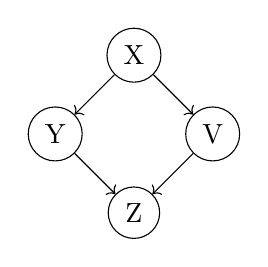
\begin{tikzpicture}
					\node[draw, circle] (X) at (0,0) {X};
					\node[draw, circle] (Y) at (-1,-1) {Y};
					\node[draw, circle] (Z) at (0,-2) {Z};
					\node[draw, circle] (V) at (1,-1) {V};
					
					\draw[->] (X) -- (Y);
					\draw[->] (Y) -- (Z);
					\draw[->] (V) -- (Z);
					\draw[->] (X) -- (V);
				
	\end{tikzpicture}	
	\caption{$Ind(Y;V|X)$, $Ind(Z;X | \left\{Y,V \right\})$, $Ind(X;Z | \emptyset)$ etc.}
\end{figure}

	\begin{definition}A node $X$ of a path $p$ in the DAG is called a \textbf{collider} if the previous and next nodes of $X$ in the path are into $X$.
\end{definition}

\begin{definition}
	A node $X$ of a path $p$ in the DAG is called an \textbf{unshielded collider} if the previous and next nodes $Y,Z$ of $X$ in the path are into $X$ and $Y$ and $Z$ are not adjacent.
\end{definition}


\begin{definition}
	A path p from X to Y is \textbf{blocked} by a set of nodes $\mathbf{Z}$ (possibly empty), if some node on $p$:
	\begin{enumerate}
		\item is a collider and neither it or any of its descendants are in $\mathbf{Z}$, or
		\item is not a collider and is in $\mathbf{Z}$
	\end{enumerate}
\end{definition}

\begin{definition}
	If a path $p$ is not blocked by a set of nodes $\mathbf{Z}$, it is said to be \textbf{active}.
\end{definition}

E.g The path $X \rightarrow Y \rightarrow Z$ is blocked by $\mathbf{Y}$, $Y \rightarrow Z \leftarrow V$ is blocked by $\mathbf{Z}=\emptyset$ etc.

\section{D-separation}

\begin{definition}[d-separation criterion]Two nodes $X$ and $Y$ are d-separated by $\mathbf{Z}$ iff every path from $X$ to $Y$ is blocked by $\mathbf{Z}$. Otherwise, we say they are \textbf{d-connected}.
\end{definition}
	
When learning causal DAGs from data, \textbf{faithfulness} and \textbf{causal sufficency} is assumed. For the first one, given a causally sufficient set of variables $\mathcal{U}$ in a population $N$, \textit{every} conditional independence relation that holds in the density over $\mathcal{U}$ \textit{is entailed by the local directed Markov condition for the causal DAG of $N$}. Causal sufficiency is the \textit{asumption that there are no unobserved variables}. Unobserved variables are called \textbf{latent} or \textbf{hidden} variables. The fact that DAGs are unable to adequately capture latent confounders becomes apparent in the example at Figure \ref{fig:dag-conf}. MAGs are able to drop the causal sufficiency assumption and are closed under marginalizing and conditioning.

\begin{figure}
\begin{multicols}{2}
	\begin{center}
		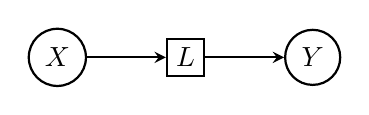
\begin{tikzpicture}[->,>=stealth,thick]
			% X -> L -> Y
			\node[draw, circle] (XLY1) {$X$};
			\node[draw, rectangle,right=of XLY1] (L1) {$L$};
			\node[draw, circle,right=of L1] (Y1) {$Y$};
			
			\draw[->] (XLY1) -- (L1);
			\draw[->] (L1) -- (Y1);
		\end{tikzpicture}
	\columnbreak
	
		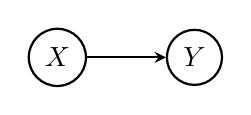
\begin{tikzpicture}[->,>=stealth,thick]
			% X <-> Y
			\node[draw, circle] (XY1) {$X$};
			\node[draw, circle,right=of XY1] (Y1) {$Y$};
			
			\draw[->] (XY1) -- (Y1);
		\end{tikzpicture}
	\end{center}
\end{multicols}

\begin{multicols}{2}
	\begin{center}
		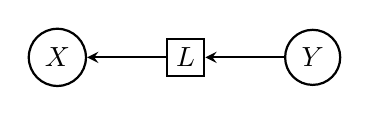
\begin{tikzpicture}[->,>=stealth,thick]
			% X <-> L <-> Y
			\node[draw, circle] (XLY2) {$X$};
			\node[draw, rectangle,right=of XLY2] (L2) {$L$};
			\node[draw, circle,right=of L2] (Y2) {$Y$};
			
			\draw[<-] (XLY2) -- (L2);
			\draw[<-] (L2) -- (Y2);
		\end{tikzpicture}
	
	    \columnbreak
	    
		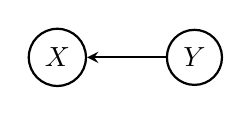
\begin{tikzpicture}[->,>=stealth,thick]
			% X <-> Y
			\node[draw, circle] (XY2) {$X$};
			\node[draw, circle,right=of XY2] (Y3) {$Y$};
			
			\draw[<-] (XY2) -- (Y3);
		\end{tikzpicture}
	\end{center}
\end{multicols}

\begin{multicols}{2}
		\begin{center}
		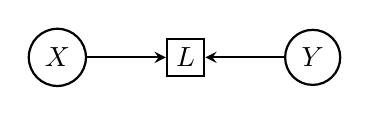
\begin{tikzpicture}[->,>=stealth,thick]
			% X <-> L <-> Y
			\node[draw, circle] (XLY2) {$X$};
			\node[draw, rectangle,right=of XLY2] (L2) {$L$};
			\node[draw, circle,right=of L2] (Y2) {$Y$};
			
			\draw[->] (XLY2) -- (L2);
			\draw[<-] (L2) -- (Y2);
		\end{tikzpicture}
	\end{center}
    \columnbreak
	\begin{center}
		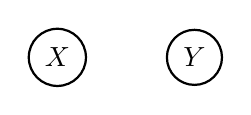
\begin{tikzpicture}[->,>=stealth,thick]
			% X <-> Y
			\node[draw, circle] (XY2) {$X$};
			\node[draw, circle,right=of XY2] (Y3) {$Y$};
			
		\end{tikzpicture}
	\end{center}
\end{multicols}

\begin{multicols}{2}
	\begin{center}
		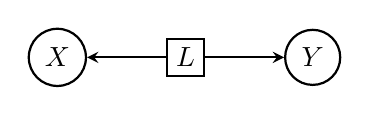
\begin{tikzpicture}[->,>=stealth,thick]
			% X <-> L <-> Y
			\node[draw, circle] (XLY2) {$X$};
			\node[draw, rectangle,right=of XLY2] (L2) {$L$};
			\node[draw, circle,right=of L2] (Y2) {$Y$};
			
			\draw[<-] (XLY2) -- (L2);
			\draw[->] (L2) -- (Y2);
		\end{tikzpicture}
	\end{center}
	
	\columnbreak
	
	\begin{center}
		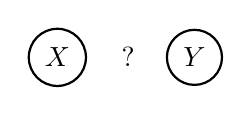
\begin{tikzpicture}[->,>=stealth,thick]
			\node[draw, circle] (XY2) {$X$};
			\node[draw, circle,right=of XY2] (Y3) {$Y$};
			\node at (0.9,0) {?};
		\end{tikzpicture}
	\end{center}
\end{multicols}
\label{fig:dag-conf}
\caption{Illustrations for the presence of a hidden confounder $L$ for two variables $X,Y$. In the first case, where $X$ indirectly causes $Y$ with $L$ acting as a mediator, we observe that $Dep(X,Y)$ so we infer $X \rightarrow Y$, and similarly $X \leftarrow Y$ in the second case. In the third case where $X$ and $Y$ share a hidden common effect, we infer $Indep(X,Y)$ and thus discover no edge between $X$ and $Y$. However, in the case of $L$ being a hidden common cause of $X$ and $Y$, there exists no DAG that captures the dependencies.}
\end{figure}

\section{Mixed Graphs}

\begin{definition}A (directed) \textbf{mixed graph} $\mathcal{G}$ is a graph that may contain two kinds of edges: directed edges ($\rightarrow$) and bi-directed edges ($\leftrightarrow$).
\end{definition}

\begin{itemize}
	\item Between any two vertices there is at \textbf{most one edge}.
	\item The two ends of an edge we call \textbf{marks}.
	\item There are two kinds of marks: \textbf{arrowhead} ($>$) and \textbf{tail} ($-$).
	\item We say an edge is \textbf{into} (\textbf{out of}) a vertex if the mark of the edge at the vertex is an arrowhead (or tail).
\end{itemize}

	If $X \rightarrow Y$ then $X$ is called a \textbf{parent} of $Y$. If $X \leftarrow Y$ then $X$ is called a \textbf{child} of $Y$. If $X \leftrightarrow Y$ then $X$ is called a \textbf{sibling} of $Y$.

\begin{equation*}
	\begin{cases}
		\textbf{pa}_{\mathcal{G}}(v) = \left\{ w : ~w \rightarrow v\right\} \\
		\textbf{sp}_{\mathcal{G}}(v) = \text{sib}_{\mathcal{G}}(v)= \left\{ w: ~w \leftrightarrow v \right\} \\
		\textbf{an}_{\mathcal{G}}(v) = \left\{ w: ~w \rightarrow \ldots \rightarrow v \text{ or } w = v\right\} \\
		\textbf{de}_{\mathcal{G}}(v) = \left\{ w: v \rightarrow \ldots \rightarrow w \text{ or } w = v \right\} \\
		\textbf{dist}_{\mathcal{G}}(v) = \left\{ w: w \leftrightarrow \ldots \leftrightarrow v \text{ or } w = v \right\}
	\end{cases}
	\text{are the} 
	\begin{cases}
		\textbf{parents} \\
		\textbf{spouses } \text{or} \textbf{ siblings} \\
		\textbf{ancestors} \\
		\textbf{descendants} \\
		\textbf{districts}
	\end{cases}
	\text{ of } v \in \mathcal{G}.
\end{equation*}

\begin{definition}\label{def:ancestral}
	A vertex $X$ is said to be an \textbf{ancestor} of a vertex $Y$, denoted $X \in \textbf{an}(Y)$, if either there exists a directed path $X \rightarrow \cdots \rightarrow Y$ from $X$ to $Y$, or $X=Y$. Similarly, $Y$ is called a \textbf{descendant} of $X$, denoted as $Y \in \textbf{de}(X)$.
\end{definition}

\begin{definition}
	A graph $\mathcal{G}$ is called an \textbf{acyclic directed mixed graph (ADMG)} if it is \textit{acyclic} and contains \textit{only directed and bidirected edges.}
\end{definition}

	\begin{definition}A mixed (directed) graph is an \textbf{ancestral graph} if:
	\begin{itemize}
		\item there are no directed cycles;
		\item whenever there is an edge $X \leftrightarrow Y$, then there is no directed path from $X$ to $Y$ or from $Y$ to $X$ (no almost directed cycles), that is, $\forall ~v \in \mathcal{V}, \text{sib}_\mathcal{G}(v) \cap \text{an}_\mathcal{G}(v) = \emptyset$.
	\end{itemize}
\end{definition}

\begin{multicols}{2}
	
	\begin{minipage}{\linewidth}
		\begin{figure}[H]
			\centering
			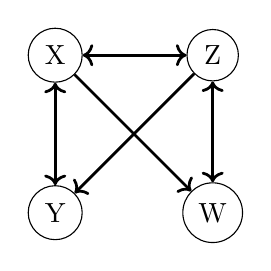
\begin{tikzpicture}
				\node[circle, draw] (X1) at (0, 0) {X};
				\node[circle, draw] (Z1) at (2, 0) {Z};
				\node[circle, draw] (Y1) at (0, -2) {Y};
				\node[circle, draw] (W1) at (2, -2) {W};
				\draw[->, line width=1pt] (X1) -- (W1);
				\draw[<->, line width=1pt] (Z1) -- (W1);
				\draw[->, line width=1pt] (Z1) -- (Y1);
				\draw[<->, line width=1pt] (X1) -- (Y1);
				\draw[<->, line width=1pt] (Z1) -- (X1); 
			\end{tikzpicture}
			\caption{An ancestral graph.}
		\end{figure}
	\end{minipage}
	
	\columnbreak
	
	\begin{minipage}{\linewidth}
		\begin{figure}[H]
			\centering
			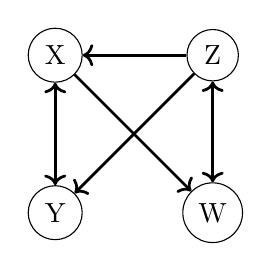
\begin{tikzpicture}
				\node[circle, draw] (X2) at (0, 0) {X};
				\node[circle, draw] (Z2) at (2, 0) {Z};
				\node[circle, draw] (Y2) at (0, -2) {Y};
				\node[circle, draw] (W2) at (2, -2) {W};
				\draw[->, line width=1pt] (X2) -- (W2);
				\draw[<->, line width=1pt] (Z2) -- (W2);
				\draw[->, line width=1pt] (Z2) -- (Y2);
				\draw[<->, line width=1pt] (X2) -- (Y2);
				\draw[->, line width=1pt] (Z2) -- (X2);
			\end{tikzpicture}
			\caption{A non-ancestral graph.}
		\end{figure}
	\end{minipage}
	
\end{multicols}

	\begin{definition} In an ancestral graph, a nonendpoint vertex X on a path is said to be a \textbf{collider} if two arrowheads meet at X (i.e., $\rightarrow X \leftarrow, \leftrightarrow X \leftrightarrow, \leftrightarrow X \leftarrow. \rightarrow X \leftrightarrow$). All other nonendpoint vertices on a path are called \textbf{noncolliders} (i.e., $\rightarrow X \rightarrow, \leftarrow X \leftarrow, \leftarrow X \rightarrow, \leftrightarrow X \rightarrow, \leftarrow X \leftrightarrow$). A path along which every non-endpoint vertex is a collider is called a \textbf{collider path}.
\end{definition}

The direct generalization of d-separation to MAGs is the m-separation criterion (m-seperation from mixed-separation):

\begin{definition}[m-connection]In an ancestral graph, a path $\pi$ between vertices $X$ and $Y$ is active or $\textbf{m-connecting}$ relative to a (possibly empty) set of vertices $\textbf{Z}$, with $X,Y \not \in \mathbf{Z}$ if 
	
	\begin{itemize}
		\item every non-collider on $\pi$ is not a member of $\mathbf{Z}$
		\item every collider on $\pi$ is an ancestor of some member of $\mathbf{Z}$
	\end{itemize}
	Otherwise we say that $\mathbf{Z}$ \textbf{blocks} $\pi$.
\end{definition}

Example: For the ancestral graph $A \rightarrow B \leftrightarrow C \leftarrow D$: The path $\pi_1 = (A,B,C,D)$ is active relative to $\mathbf{Z} = \left\{ B,C \right\}$. The path $\pi_1$ is not m-connecting relative to $\mathbf{Z} = \emptyset$, $\mathbf{Z} = \left\{ B \right\}$ or $\mathbf{Z} = \left\{ C\right\}$.

\begin{definition}[m-separation] $X$ and $Y$ are said to be \textbf{m-separated by} $\mathbf{Z}$ if there are no active paths between $X$ and $Y$ relative to $\mathbf{Z}$, i.e if $\mathbf{Z}$ blocks all paths between $X$ and $Y$.
\end{definition}

\begin{definition}[m-separation]Two disjoint sets of variables $X$ and $Y$ are m-separated by $\mathbf{Z}$ if every variable in $\mathbf{X}$ is m-separated from every variable in $\mathbf{Y}$ by $\mathbf{Z}$.
\end{definition}

Example: For the ancestral graph $A \rightarrow B \leftarrow C \leftarrow D$, we have that: $\left\{ A\right\} \perp\!\!\!\perp_m \left\{ D \right\}$, $\left\{ A\right\} \perp\!\!\!\perp_m \left\{ D \right\} | \left\{ B \right\}$ and $\left\{ A\right\} \perp\!\!\!\perp_m \left\{ D \right\} | \left\{ C\right\}$. Since there is no active path relative to $\mathbf{Z} = \emptyset$, $\mathbf{Z} = \left\{ B \right\}$ and $\mathbf{Z} = \left\{ C \right\}$ respectively. Moreover, $\left\{ A\right\} \not \perp\!\!\!\perp_m \left\{ D \right\} | \left\{ B, C\right\}$ because $\pi_1 = (A,B,C,D)$ is active relative to $\mathbf{Z} = \left\{ B,C \right\}$. \\

The notion of maximality is that every missing edge corresponds to a conditional independence relation. 

\begin{definition}[Maximality]
	An ancestral graph is \textbf{maximal} if for every pair of nonadjacent vertices $(a, b)$ there exists a set $\mathbf{Z}$ with $a, b \not \in \mathbf{Z}$ such that $a$ and $b$ are m-separated conditional on $\mathbf{Z}$ (i.e the pairwise Markov property holds).
\end{definition}

Equivalently:

\begin{definition}
	An ancestral graph $\mathcal{G}$ is said to be \textbf{maximal} if for every pair of non-adjacent vertices $(X,Y)$ there exists a set of $\mathbf{Z}$ ($X,Y \not \in \mathbf{Z}$) such that $X$ and $Y$ are m-separated conditional on $\mathbf{Z}$.
\end{definition}

\begin{multicols}{2}
	\begin{minipage}{\linewidth}
		\begin{figure}[H]
			\centering
			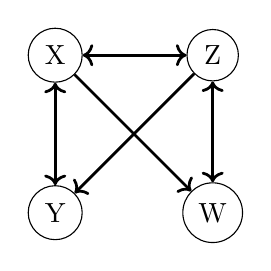
\begin{tikzpicture}
				\node[circle, draw] (X1) at (0, 0) {X};
				\node[circle, draw] (Z1) at (2, 0) {Z};
				\node[circle, draw] (Y1) at (0, -2) {Y};
				\node[circle, draw] (W1) at (2, -2) {W};
				\draw[->, line width=1pt] (X1) -- (W1);
				\draw[<->, line width=1pt] (Z1) -- (W1);
				\draw[->, line width=1pt] (Z1) -- (Y1);
				\draw[<->, line width=1pt] (X1) -- (Y1);
				\draw[<->, line width=1pt] (Z1) -- (X1);
			\end{tikzpicture}
			\caption{A non-maximal ancestral graph.}
			\label{fig:non-maximal-ancestral}
		\end{figure}
	\end{minipage}
	
	\columnbreak
	
	\begin{minipage}{\linewidth}
		\begin{figure}[H]
			\centering
			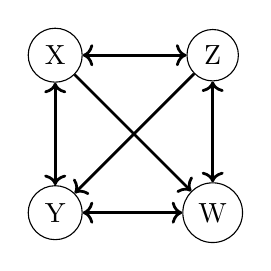
\begin{tikzpicture}
				\node[circle, draw] (X2) at (0, 0) {X};
				\node[circle, draw] (Z2) at (2, 0) {Z};
				\node[circle, draw] (Y2) at (0, -2) {Y};
				\node[circle, draw] (W2) at (2, -2) {W};
				\draw[->, line width=1pt] (X2) -- (W2);
				\draw[<->, line width=1pt] (Z2) -- (W2);
				\draw[->, line width=1pt] (Z2) -- (Y2);
				\draw[<->, line width=1pt] (X2) -- (Y2);
				\draw[<->, line width=1pt] (Z2) -- (X2);
				\draw[<->, line width=1pt] (Y2) -- (W2);
			\end{tikzpicture}
			\caption{A maximal ancestral graph.}
			\label{fig:non-maximal-vs-maximal}
		\end{figure}
	\end{minipage}
\end{multicols}

To show that the left AG in Figure \ref{fig:non-maximal-vs-maximal} is non-maximal, notice that the only pair of non-adjacent vertices is $(Y,W)$. $\mathbf{Z} = \left\{ X\right\}$, $\pi_1$ is \textit{not an active path} since $Z \not \in \textbf{an}(X)$ but $\pi_2 = (Y,Z,W)$ is active since there are no colliders in $\pi_2$, $Z$ is a non-collider for $\pi_2$ and $Z \not \in \mathbf{Z}$. For $\mathbf{Z} = \left\{ X, Z\right\}$, $\pi_1 = (Y,X,Z,W)$ is a path that m-connects $Y$ and $W$. For $\mathbf{Z} = \left\{ Z\right\}$, $\pi_3 = (Y,Z,W)$ is an active path as there are no colliders in $\pi_3$, $X$ is a non-collider for $\pi_3$ and $X \not \in \mathbf{Z}$. For $\mathbf{Z} = \emptyset$, $\pi_1$ and $\pi_3$ are active paths. The reader should have noticed so far that DAGs are a subset of MAGs (a MAG with no bidirected edges is a MAG).

\begin{theorem}
	A directed edge $X \rightarrow Y$ from some node $X$ into another node $Y$ denotes that $Y$ is \textit{not} an ancestor of $X$.
\end{theorem}
\begin{proof}
	Let $\mathcal{M}$ be a MAG and $X,Y$ two nodes on $\mathcal{M}$. Without loss of generality, assume $X \rightarrow Y$ is in $\mathcal{M}$ and $Y$ is an ancestor of $X$. Then there is a directed path from $Y$ to $X$, but this means that the MAG $\mathcal{G}$ contains a directed cycle, contradiction. Hence if $X \rightarrow Y$, $Y$ is not an ancestor of $X$.
\end{proof}

With a similar proof as before, we can show that a bidirected edge $X \leftrightarrow Y$ between some nodes $X$ and $Y$ denotes that a) $X$ is \textit{not} an ancestor of $Y$ and b) $Y$ is \textit{not} an ancestor of $X$.

\begin{theorem}A directed edge $X \rightarrow Y$ between some nodes $X$ and $Y$ denotes that 
	\begin{enumerate}
		\item $X$ is an ancestor of $Y$
		\item $Y$ is not an ancestor of $X$
		\item The above does not rule out \textbf{possible latent confounding} between $X$ and $Y$.
	\end{enumerate}
\end{theorem}

\begin{theorem}A bidirected edge $X \leftrightarrow Y$ between some nodes $X$ and $Y$ denotes that 
\begin{enumerate}
	\item $X$ is \textit{not} an ancestor of $Y$
	\item $Y$ is \textit{not} an ancestor of $X$
	\item $X$ and $Y$ are \textbf{confounded}.
\end{enumerate}
\end{theorem}

Maximal ancestral graphs (MAGs) are maximal in the sense that \textbf{no additional edge may be added to the graph without changing the independence model} induced by the MAG.

\begin{theorem}If $\mathcal{M} = (V,E)$ is a maximal ancestral graph and $\mathcal{M}$ is a subgraph of $\mathcal{G}^* = (V,E^*)$, then $\mathbf{I}_m (\mathcal{M}) = \mathbf{I}_m(\mathcal{M}^*)$ implies that $\mathcal{M} = \mathcal{M}^*$.
\end{theorem}

\begin{theorem}If $\mathcal{G}$ is an ancestral graph then there exists a \textbf{unique} maximal ancestral graph $\mathcal{M}$ formed by adding $\leftrightarrow$ edges to $\mathcal{G}$ such that $\mathbf{I}_m (\mathcal{M}) = \mathbf{I}_m(\mathcal{G})$
\end{theorem}

Maximality is closely related to the definition of (primitive) inducing paths, which is used on the algorithms we will be studying.

\begin{definition}[inducing paths]
	An \textbf{inducing path $\pi$ relative to a set} $\mathbf{L}$ between two vertices $X$ and $Y$ in an ancestral graph $\mathcal{G}$, is a path on which every non-endpoint vertex, \textit{not} in $\mathbf{L}$ is both a collider on $\pi$ and an ancestor of \textit{at least one} of the endpoints $X$ and $Y$.
\end{definition}

From the definition, we notice that any single-edge path is trivially an inducing path relative to any set of vertices. As a simplification of the terminology, inducing paths relative to the empty set will be referred as (primitive) \textbf{inducing paths}. Also it may not be a single path but a collection of paths.

For example, in figure \ref{fig:non-maximal-ancestral} the path $(Y,Z,W)$ is an inducing path relative to $\left\{ Z\right\}$ but not an inducing path relative to the empty set (because $Z$ is not a collider). The path $(Y,X,Z,W)$ is an inducing path relative to the empty set, because both $X$ and $Z$ are colliders on the path, $X$ is an ancestor of $W$, and $Z$ is an ancestor of $Y$.

\begin{definition}A mixed graph is called a maximal ancestral graph (MAG) if:
	\begin{itemize}
		\item The graph does not contain any directed or almost directed cycles (ancestral) and
		\item there is \textit{no inducing path} between any two non-adjacent vertices (maximal)
	\end{itemize}
\end{definition}

%A property of MAGs is that they represent the marginal independence models of a DAG over $\mathbf{V} = \mathbf{O} \cup \mathbf{L}$ \cite{richardson2002}. This means that given any DAG $\mathcal{D}$ over $\mathbf{V} = \mathbf{O}\cup \mathbf{L}$ there is a MAG $\mathcal{M}$ over $\mathbf{O}$ alone, such that for any disjoint sets $\mathbf{X, Y, Z \subset O, X}$ and $\mathbf{Y}$ are d-separated by $\mathbf{Z}$ in $\mathcal{D}$ iff they are m-separated by $\mathbf{Z}$ in the MAG $\mathcal{M}$. This can be constructed as follows:

%	\begin{algorithm}[H]
%	\caption{DAGs to MAGs}
%	\label{alg:dag-to-mag}
%	\begin{algorithmic}[1]
%		\Require A DAG $\mathcal{D}$ over $\mathbf{O} \cup \mathbf{L}$
%		\Ensure A MAG $\mathcal{M}_\mathcal{D}$ over $\mathbf{O}$
%		\ForAll{pairs of variables $X, Y \in \mathbf{O}$}
%		\State $\mathcal{M}$ is adjacent to $X$ and $Y$ iff there is an inducing path between them relative to $\mathbf{L}$ in $\mathcal{D}$
%		\EndFor
%		\ForAll{pairs of adjacent variables $X, Y$ in $\mathcal{M}$}
%		\If{$X$ is an ancestor of $Y$ in $\mathcal{D}$}
%		\State Orient the edge as $X \to Y$ in $\mathcal{M}$
%		\ElsIf{$Y$ is an ancestor of $X$ in $\mathcal{D}$}
%		\State Orient the edge as $X \leftarrow Y$ in $\mathcal{M}$
%		\Else
%		\State Orient the edge as $X \leftrightarrow Y$ in $\mathcal{M}$
%		\EndIf
%		\EndFor
%	\end{algorithmic}
%\end{algorithm}

%\begin{figure}
%   \begin{minipage}{0.48\textwidth}
%	\centering
%	\begin{tikzpicture}
%		\node[circle, draw] (X) at (0, 0) {X};
%		\node[circle, draw] (Y) at (1, -1) {Y};
%		\node[circle, draw] (L1) at (2, 0) {$L_1$};
%		\node[circle, draw] (Z) at (3, -1) {Z};
%		\node[circle, draw] (W) at (4, 0) {W};
%		\draw[->, line width=1pt] (X) -- (Y);
%		\draw[->, line width=1pt] (L1) -- (Y);
%		\draw[->, line width=1pt] (L1) -- (Z);
%		\draw[->, line width=1pt] (Z) -- (Y);
%		\draw[->, line width=1pt] (W) -- (Z);
%	\end{tikzpicture}
%	\caption{A DAG $\mathcal{D}$ over $\mathbf{O\cup L}$ where $\mathbf{L} = \left\{ L_1\right\}$.}
%\end{minipage}
%\hfill
%\begin{minipage}{0.48\textwidth}
%	\centering
%	\begin{tikzpicture}
%		\node[circle, draw] (X) at (0, 0) {X};
%		\node[circle, draw] (Y) at (1, -1) {Y};
%		\node[circle, draw] (Z) at (3, -1) {Z};
%		\node[circle, draw] (W) at (4, 0) {W};
%		\draw[->, line width=1pt] (X) -- (Y);
%		\draw[->, line width=1pt] (Z) -- (Y);
%		\draw[->, line width=1pt] (W) -- (Z);
%	\end{tikzpicture}
%	\caption{A MAG $\mathcal{D}$ over $\mathbf{O}$ from the DAG $\mathcal{D}$.}
%\end{minipage}
%\end{figure}

%One can see that if two variables share a hidden common cause and there is a directed edge between them, then the MAG only keeps the directed edge. Because MAGs represent ancestral relationships, a directed edge dominates a bi-directed edge. Moreover, there may also exist edges in the MAG that are not present in the underlying causal model.

\section{Markov Equivalence}

Just like DAGs (which are a subset of MAGs), several MAGs can encode the same conditional independencies via m-separation (as various DAGs can encode the same conditional independencies via d-separation) and are not distinguishable only by correlational patterns.

\begin{definition}Two MAGs $\mathcal{G}_1,\mathcal{G}\_2$ over the same set of vertices are called \textbf{Markov equivalent} if for any three
	disjoint sets of vertices $X,Y,Z$, $X$ and $Y$ are m-separated by $Z$ in $\mathcal{G}_1$ iff $X$ and $Y$ are m-separated by $Z$ in $\mathcal{G}_2$.
\end{definition}

\begin{definition}In a MAG, a path consisting of a triple of vertices $X,Y,Z$ is said to be \textbf{unshielded} if $X$ and $Z$ are not adjacent.
\end{definition}

\begin{definition}A vertex $Y$ is called an \textbf{unshielded collider} if the vertices $X, Z$ are into $Y$ and $X$ and $Z$ are not adjacent.
\end{definition}

\begin{definition}[discriminating paths]In a MAG $\mathcal{G}$, a path $\pi = (x, q_1,\ldots, q_p,b, y), ~p \geq 1$ is called a \textbf{discriminating path for} $b$ if:
	\begin{itemize}
		\item $x$ is not adjacent to $y$, and
		\item every vertex $q_i$, $1 \leq i \leq p$ is a collider on $\pi$ and a parent of $y$.
	\end{itemize}
\end{definition}

\begin{figure}[h]
	\centering
	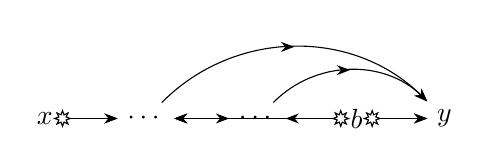
\begin{tikzpicture}[>=Stealth, auto, node distance=0.7cm]	
		\node (x) {$x$};
		\node[right=of x] (a1) {$\cdots$};
		\node[right=of a1] (a2) {$\cdots$};
		\node[right=of a2] (b) {$b$};
		\node[right=of b] (y) {$y$};
		
		\draw[->] (x) -- (a1);
		\draw[<->] (a1) -- (a2);
		\draw[->] (b) -- (a2);
		\draw[->] (b) -- (y);
		
		\draw[->, postaction={decorate,decoration={markings,mark=at position 0 with {\node[draw,fill=white,star,star points=8,star point ratio=2,inner sep=1pt]{};}}}] (x) to (a1);	
		
		\draw[->, postaction={decorate,decoration={markings,mark=at position 0 with {\node[draw,fill=white,star,star points=8,star point ratio=2,inner sep=1pt]{};}}}] (b) to (a1);
		
		\draw[->, postaction={decorate,decoration={markings,mark=at position 0 with {\node[draw,fill=white,star,star points=8,star point ratio=2,inner sep=1pt]{};}}}] (b) to (y);
				
		\draw[->, bend left=45, postaction={decorate,decoration={markings,mark=at position 0.5 with {\arrow{>}}}}] (a1) to (y);
		\draw[->, bend left=45, postaction={decorate,decoration={markings,mark=at position 0.5 with {\arrow{>}}}}] (a2) to (y);
	\end{tikzpicture}
    \caption{A discriminating path $\pi = (x, q_1,\ldots, q_p,b, y), ~p \geq 1$ for $b$.}
    \label{fig:discr}
\end{figure}

Notice that a discriminating path is not a single path but potentially a collection of paths (if more than one exist). For Markov Equivalence in MAGs, it is known due to Verma \& Pearl \cite{verma1990} that:

\begin{theorem}[\cite{verma1990}] Two DAGs $\mathcal{G}_1$ and $\mathcal{G}_2$ are Markov equivalent iff
	\begin{enumerate}
		\item $\mathcal{G}_1$ and $\mathcal{G}_2$ have the same adjacencies
		\item $\mathcal{G}_1$ and $\mathcal{G}_2$ have the same unshielded colliders
	\end{enumerate}
\end{theorem}

For MAGs, although having the same adjacencies and unshielded colliders is necessary, it is not sufficient for Markov equivalence. Consider the MAGs $x \leftrightarrow q \rightarrow y \leftrightarrow b$ with a bidirected edge $q \leftrightarrow b$ and $x \rightarrow q \rightarrow y \leftarrow b$ with a directed edge $q \leftarrow b$. The two MAGs share the same adjacencies and unshielded colliders. But in the first graph, $q$ m-separates $x$ and $y$ but $q$ m-connects $x$ and $y$ in the second graph. The Verma \& Pearl criterion on DAGs is extended to MAGs with the Spirtes-Richardson Criterion (SRC) (\cite{spirtes1996}):

\begin{theorem}[Spirtes-Richardson Criterion \cite{spirtes1996}]
	\label{thrm:spirtes1996}
	Two MAGs $\mathcal{G}_1$ and $\mathcal{G}_2$ are Markov equivalent iff
	\begin{enumerate}
		\item $\mathcal{G}_1$ and $\mathcal{G}_2$ have the same adjacencies
		\item $\mathcal{G}_1$ and $\mathcal{G}_2$ have the same unshielded colliders and
		\item if $\pi$ forms a discriminating path for $b$ in $\mathcal{G}_1$ and $\mathcal{G}_2$, then $b$ is a collider on the path $\pi$ in $\mathcal{G}_1$ if and only if it is a collider on the path $\pi$ in $\mathcal{G}_2$.
	\end{enumerate}
\end{theorem}

Markov Equivalent MAGs form a Markov equivalence class that can be described uniquely by a \textbf{partial ancestral graph (PAG)}. A PAG $\mathcal{P}$ has the same adjacencies as any MAG in the Markov equivalence class described by $\mathcal{P}$. We denote all MAGs in the Markov equivalence class described by a PAG $\mathcal{G}$ by $[\mathcal{G}]$. Let \textit{partial mixed graphs} denote the class of graphs containing four types of edges: $\rightarrow$, $\leftarrow$, $\circ \rightarrow$, $\circ$ and three types of end marks: arrowhead ($>$), tail ($-$) and circle $\circ$.

\section{Ali-Spirtes-Richardson (ASR) \cite{ali2009} Algorithm}

Discriminating paths, when present in both graphs, lead directly to necessary conditions for Markov equivalence. However, a discriminating path for a given triple may not be present in all graphs within a Markov equivalence class. The authors avoid this by a recursive definition, triples in order, a sub-class of discriminating paths and associated triples (those that are “with order”) that are always present, and proving Markov equivalence combined with (i) and (ii) conditions of same adjacencies and unshielded colliders.

\begin{definition}[Definition 3.11 in \cite{ali2009}] Let \( O_i \) (\( i \geq 0 \)) be the set of triples of order \( i \) in a MAG \( \mathcal{G} \), defined recursively as follows:
	\begin{itemize}
		\item  \textbf{Order 0.} A triple \( \langle a, b, c \rangle \in O_0 \) if \( a \) and \( c \) are not adjacent.
		\item \textbf{Order \( i+1 \).} A triple \( \langle a, b, c \rangle \in O_{i+1} \) if
		\begin{enumerate}
			\item for all \( j<i+1 \), \( \langle a, b, c \rangle \notin O_j \), and,
			\item there is a discriminating path \( \langle x, q_1, \ldots, q_p, b, y \rangle \) for \( b \) with either \( \langle a, b, c \rangle = \langle q_p, b, y \rangle \) or \( \langle a, b, c \rangle = \langle y, b, q_p \rangle \) and the \( p \) colliders \(\displaystyle \langle x, q_1, q_2 \rangle, \ldots, \langle q_{p-1}, q_p, b \rangle \in \bigcup_{j\leq i} O_j \).
		\end{enumerate}
	\end{itemize}

If \( \langle a, b, c \rangle \in O_i \) then the triple is said to have order \( i \). If a triple has order \( i \) for some \( i \), then we will say that the triple has order. A discriminating path is said to have order \( i \) if, excepting \( \langle q_p, b, y \rangle \), every collider on the path has order at most \( i - 1 \), and at least one collider has order \( i - 1 \).
\end{definition}

The main theorem of the paper, in which the algorithm is based on, is the following:

\begin{theorem}[Theorem 3.7 in \cite{ali2009}]Two MAGs $\mathcal{G}_1$ and $\mathcal{G}_2$ are Markov equivalent if and only if they have the same adjacencies and the same colliders with order.
\end{theorem}

To present the Markov equivalence algorithm, we introduce the following notation:

\begin{itemize}
	\item $\text{Adj}(\mathcal{G}) = \{(x, y) \mid x \text{ and } y \text{ are adjacent in } \mathcal{G}\}$,
	\item $\text{Col}(\mathcal{G}) = \{(x, y, z) \mid x ~\circ\rightarrow y \leftarrow\circ ~z \text{ in } G\}$,
	\item $\text{OCol}(\mathcal{G}) = \{(x, y, z) \mid (x, y, z) \in \text{Col}(\mathcal{G}) \text{ and } (x, y, z) \text{ has order}\}$,
	\item $\displaystyle \text{ICol}(\mathcal{G}) = \bigcap_{\overline{\mathcal{G}} \sim \mathcal{G}}(\overline{\mathcal{G}})$
\end{itemize}

which are, respectively, the \textit{set of adjacencies, colliders, colliders with order in $\mathcal{G}$ and colliders common to all graphs in the Markov equivalence class containing} $\mathcal{G}$. In general, we have that $\text{Col}(\mathcal{G}) \subset \text{ICol}(\mathcal{G}) \subset \text{Col}(\mathcal{G})$. 

The algorithm \textit{Reachable} (Algorithm \ref{alg:asr-reachable}) outputs the vertices connected to the input vertex with a directed path, using depth-first search. The algorithm \textit{Triples} seeks to identify a superset of colliders with order and runs as follows: Line 4 locates candidate triples $(a, b, c)$. Lines 5, 6, and 7 search for collider paths and the sets “vertices” ($V$) and “edges” ($E$) in $\mathbf{D}$ correspond to edges and colliders in $\mathcal{G}$ respectively. Lines 8 and 9 search for a vertex satisfying the conditions on x.

The algorithm $\text{Reachable}(\mathbb{D},w)$ runs in $\mathcal{O}(n+e)$ (BFS). Regarding $\text{Triples}(\mathcal{G})$ (Algorithm \ref{alg:asr-triples}): Any triple appearing on a minimal m-connecting path $\pi$ has order at most $n^3$: $\pi$ contains at most $n$ vertices; hence, at most $n^2$ triples; all of the other discriminating paths involved are sections of $\pi$; and unshielded triples (of which there is at least one) are of order $0$. Thus, it is always sufficient for Markov equivalence to check that two graphs have triples of order less than $n$. Hence, the main loop in $\text{Triples}(G)$ is of complexity $\mathcal{O}(n)$. Line 4 is executed $\mathcal{O}(e^2)$ times (for each $k$) and since $E$ is of size $\mathcal{O}(e^2)$, lines 5 to 7 are also of complexity $\mathcal{O}(e^2)$. Finally, line 8 is $\mathcal{O}(e^2)$ (since $T_{k-1}$ is of size $\mathcal{O}(e^2)$) and line 9 is $\mathcal{O}(e)$. Thus overall $\mathcal{O}(ne^4)$.

%$\mathcal{O}(n(n^3 + e^2 + e^2 + e) = \mathcal{O}(n^4 + 2ne^2 + ne) = \mathcal{O}()$
	 
\section{Hu-Evans \cite{hu2020} Algorithm}

The second attempt at creating an efficient polynomial algorithm for testing Markov equivalence in MAGs was introduced by Hu and Evans \cite{hu2020} in 2020 at the Department of Statistics at the University of Oxford. The authors make use of parametrizing sets, reducing the complexity of the previous approach to $\mathcal{O}(ne^2)$. 

\begin{definition}[Induced Subgraph] Let $\mathcal{G} = (\mathcal{V},\mathcal{E})$ be an ADMG and $W \subset \mathcal{V}$. Then the \textbf{induced subgraph} $\mathcal{G}_W$ is the ADMG with vertex set $W$ and edges in $\mathcal{G}$ with endpoints both in $W$.
\end{definition}

\begin{definition}[Barren subsets]For a set of vertices $W \subset V$:  $\text{barren}_\mathcal{G}(W) = \{w \in W : \text{de}_\mathcal{G}(w) \cap W = \{w\}\}$.
\end{definition}
	
\begin{definition}[Heads]A vertex set $H$ is called a \textit{head} if (i) $\text{barren}_\mathcal{G}(H) = H$ and (ii) $H$ is contained in a single district in $\mathcal{G}_{an(H)}$ (the subgraph induced by the ancestors of $H$).
\end{definition}
	
For an ADMG $\mathcal{G}$, denote the set of all heads in $\mathcal{G}$ as $\mathcal{H}(\mathcal{G})$.
 
\begin{definition}[Tails]A tail of a head $H$ is defined as $\text{tail}(H) = (\text{dis}_{\text{an}(H)}(H)) \cup \text{pa}_{\mathcal{G}}(\text{dis}_{\text{an}(H)}(H))$.
\end{definition}

\begin{definition}[Parametrizing set]The \textit{parametrizing set $\mathcal{S(G)}$ of $\mathcal{G}$} is $$\mathcal{S(G)} = \left\{ H \cup A : h \in \mathcal{H(G)} \text{ and } \emptyset \subset A \subset \text{tail}(H) \right\} $$
\end{definition}

\begin{definition}For $k \geq 2$ define $\mathcal{S}_k(\mathcal{G}) = \left\{ S \in \mathcal{S(\mathcal{G})} : 2 \leq |S| \leq k \right\}$ the parametrizing sets of order $k$. That is, with cardinality $2$ or $3$.
\end{definition}

Finally, define the following subset of $\mathcal{S}_k(\mathcal{G})$:

\begin{definition}
 $\mathcal{\tilde{S}}_3(\mathcal{G}) = \left\{ S \in \mathcal{S}_3(\mathcal{G}) \text{ where there are $1$ or $2$ adjacencies between the vertices in } S \right\}$.
\end{definition}

In a MAG $\mathcal{M}$, a pair of vertices is in $\mathcal{S(M)}$ iff they are adjacent. Recall condition (iii) from the Spirtes-Richardson Criterion (Theorem \ref{thrm:spirtes1996}): If $\pi = (x,q_i,\ldots,q_m,b,y)$ with $m \geq 1$ forms a discriminating path for $b$, then $\pi$ is a subgraph of the following collection of paths: 

$$x ~\circ \rightarrow q_1 \leftrightarrow \ldots q_i \rightarrow y, ~1 \leq i \leq m$$

$$x ~\circ \rightarrow q_1 \leftrightarrow \ldots q_m \leftarrow \circ ~b ~\circ \rightarrow y$$

The main takeaway of the paper is that conditional independencies in MAGs (induced from $m$-separation) correspond to the missing sets of the form $\left\{ a, b \right\} \cup C'$ where $a \indep_m b | C$ and $C' \subset C$. Hence the Markov equivalence algorithm works on the fact that equivalent graphs should have the same parametrizing sets, with equivalence relationships refined to consider only $\mathcal{S}_3$ or $\mathcal{\hat{S}}_3$. This results in the following central Theorem:

\begin{theorem}[3.2, Hu and Evans, 2020 \cite{hu2020}]\label{thm:hu}Let $\mathcal{G}_1$ and $\mathcal{G}_2$ be two MAGs. Then $\mathcal{G}_1$ and $\mathcal{G}_2$ are Markov equivalent iff $\tilde{S}(\mathcal{G}_1) = \tilde{S}(\mathcal{G}_2)$.
\end{theorem}

The above shows that in order to show Markov equivalence one has to compute the parametrizing sets of the MAGs, which in turn means to compute the corresponding heads and tails. However since their cardinality is not polynomial to the size of the graph, they reduce to sets of cardinality $2$ or $3$, and even further, with $1$ or $2$ adjacencies between the vertices, that is, considering only $\mathcal{S}_3$.

\begin{corollary}[3.2.1, Hu and Evans, 2020 \cite{hu2020}]Let $\mathcal{G}_1$ and $\mathcal{G}_2$ be two MAGs. Then $\mathcal{G}_1$ and $\mathcal{G}_2$ are Markov equivalent iff $\mathcal{S}_3(\mathcal{G}_1) = \mathcal{S}_3(\mathcal{G}_2) \Leftrightarrow \mathcal{\tilde{S}}_3(\mathcal{G}_1) = \mathcal{\tilde{S}}_3(\mathcal{G}_2)$.
\end{corollary}

To prove the Theorem and its corollary hold, the following propositions are used:

\begin{proposition}[3.3, Hu and Evans, 2020 \cite{hu2020}] Let $\mathcal{G} = (\mathcal{V},\mathcal{E})$ be a MAG. For a set $W \subset \mathcal{V}$, $W \not \in \mathcal{S}(\mathcal{G})$ if and only if there exist two vertices $a,b \in W$ such that they can be m-separated by a set $C$ such that $a,b \not \in C$ with $W \subset C \cup \left\{ a,b\right\}$.
\end{proposition}

\begin{proposition}[3.4, Hu and Evans, 2020 \cite{hu2020}]For a MAG $\mathcal{G} = (\mathcal{V},\mathcal{E})$
	\begin{enumerate}
		\item Any $a,b \in \mathcal{V}$ are adjacent iff $\left\{ a, b\right\} \in \mathcal{S}(\mathcal{G})$
		\item For any unshielded triple $(a,b,c)$, $\left\{ a, b, c \right\} \in \mathcal{S}(\mathcal{G})$ iff $b$ is a collider on that triple
		\item if $\pi$ forms a discriminating path for $b$ with two end vertices $x,y \in \mathcal{V}$ then $\left\{ x, b, y\right\} \in \mathcal{S}(\mathcal{G})$ iff $b$ is a collider on the path $\pi$. 
	\end{enumerate}
	
\end{proposition}

\begin{proof}[Proof of Theorem \ref{thm:hu}]
	The proofs follow from Propositions 3.3 and 3.4 in \cite{hu2020}: For the direct of Theorem 3.2, proposition 3.3 ensures that sets that do not exist in $\mathcal{S}(\mathcal{G})$ are due to m-separation, hence for MAGs $\mathcal{G}_1$ and $\mathcal{G}_2$ there must hold $\mathcal{S}(\mathcal{G}_1) = \mathcal{S}(\mathcal{G}_2)$. For the inverse, proposition 3.4 implies that any violations in Theorem 3.1 result in different parameterizing sets, hence equality must hold.
\end{proof}

\begin{multicols}{2}
	\begin{minipage}{\linewidth}
		\begin{figure}[H]
			\centering
			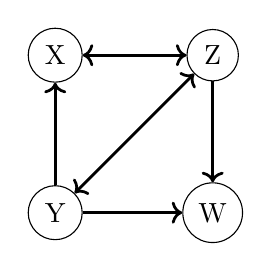
\begin{tikzpicture}
				\node[circle, draw] (X1) at (0, 0) {X};
				\node[circle, draw] (Z1) at (2, 0) {Z};
				\node[circle, draw] (Y1) at (0, -2) {Y};
				\node[circle, draw] (W1) at (2, -2) {W};
				\draw[<->, line width=1pt] (X1) -- (Z1);
				\draw[->, line width=1pt] (Z1) -- (W1);
				\draw[<->, line width=1pt] (Z1) -- (Y1);
				\draw[->, line width=1pt] (Y1) -- (W1);
				\draw[->, line width=1pt] (Y1) -- (X1);
			\end{tikzpicture}
			\caption{Maximal ancestral graph (i).}
			\label{fig:mag-head-tail1}
		\end{figure}
	\end{minipage}
	
	\columnbreak
	
	\begin{minipage}{\linewidth}
		\begin{figure}[H]
			\centering
			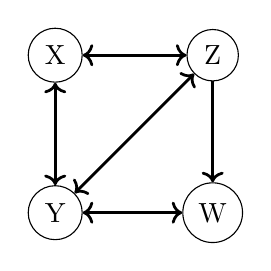
\begin{tikzpicture}
				\node[circle, draw] (X2) at (0, 0) {X};
				\node[circle, draw] (Z2) at (2, 0) {Z};
				\node[circle, draw] (Y2) at (0, -2) {Y};
				\node[circle, draw] (W2) at (2, -2) {W};
				\draw[->, line width=1pt] (Z2) -- (W2);
				\draw[<->, line width=1pt] (X2) -- (Z2);
				\draw[<->, line width=1pt] (X2) -- (Y2);
				\draw[<->, line width=1pt] (Y2) -- (W2);
				\draw[<->, line width=1pt] (Z2) -- (Y2);
			\end{tikzpicture}
			\caption{Maximal ancestral graph (ii).}
			\label{fig:mag-head-tail2}
		\end{figure}
	\end{minipage}
\end{multicols}

\begin{figure}
	\centering
	\begin{minipage}{0.45\textwidth}
		\centering
		\begin{tabular}{ |p{1cm}|p{1cm}|  }
			\hline
			\multicolumn{2}{|c|}{MAG (i)} \\
			\hline
			Heads & Tails\\
			\hline
			X & Y \\
			Z & $\emptyset$ \\
			Y & $\emptyset$ \\
			W & Z,Y \\ 
			X,Z & Y \\
			Z,Y & $\emptyset$ \\
			\hline
		\end{tabular}
	\end{minipage}
	\begin{minipage}{0.45\textwidth}
		\centering
		\begin{tabular}{ |p{1cm}|p{1cm}|  }
			\hline
			\multicolumn{2}{|c|}{MAG (ii)} \\
			\hline
			Heads & Tails\\
			\hline
			X & $\emptyset$ \\
			Z & $\emptyset$ \\
			Y & $\emptyset$ \\
			W & Z \\ 
			X,Z & $\emptyset$ \\
			X,Y & $\emptyset$ \\
			Z,Y & $\emptyset$ \\
			Y,W & Z \\
			X,Z,Y & $\emptyset$ \\
			X,Y,W & Z \\
			\hline
		\end{tabular}
	\end{minipage}
   \label{fig:mag-head-tail3}
	\caption{Heads and tails sets of the MAGs (i) and (ii) in Figures \ref{fig:mag-head-tail1} (left) and \ref{fig:mag-head-tail2} (right) respectively, which are then used to compute the parametrizing sets of each MAG.}
\end{figure}

For example, Figures \ref{fig:mag-head-tail1} and \ref{fig:mag-head-tail2} show two non-Markov equivalent MAGs. The heads and tails sets are computed in Table \ref{fig:mag-head-tail3}. The parametrizing set for MAG (i) (Figure \ref{fig:mag-head-tail1}) $\mathcal{S}(\mathcal{G}_1)$ consist of the sets $\left\{ X \right\}, \left\{ Z\right\}, \left\{ Y\right\}, \left\{ W\right\}$, $\left\{ X,Z \right\}, \left\{ X, Y\right\}, \left\{ Z, Y\right\}$, $\left\{ Z,W \right\}, \left\{ Y, W\right\}$, $\left\{ X,Z,Y \right\}, \left\{ Z,Y,W\right\}$. Similarly, for the MAG (ii) (Figure \ref{fig:mag-head-tail2}) we obtain the sets $\left\{ X \right\}, \left\{ Z\right\}$, $\left\{ Y\right\}, \left\{ W\right\}, \left\{ X,Z \right\}, \left\{ X, Y\right\}, \left\{ Z, Y\right\}$, $\left\{ Z,W \right\}$, $\left\{ Y, W\right\}, \left\{ X,Z,Y \right\}$, $\left\{ X,Y,W\right\}, \left\{ Z,Y,W\right\}$, $\left\{X,Y,Z,W \right\}$. Since they are not equal, the two MAGs are not Markov equivalent (which is also sufficient to show using only the sets $\mathcal{\tilde{S}}_3(\mathcal{G}_1)$ and $\mathcal{\tilde{S}}_3(\mathcal{G}_2)$).

The complexity of Algorithm \ref{alg:hu} the following: The loop from lines $2$ to $9$ runs in $\mathcal{O}(e^2)$ time (in the worst case a vertex has $n-1$ parents, hence $\mathcal{O}(n^2 \cdot n^2) = \mathcal{O}(n^4)$). The loop from line $11$ to $24$ runs in $\mathcal{O}(e)$ because there are at most $e$ bidirected edges. The set of tails for $\left\{u,w\right\}$ runs in $\mathcal{O}(n+e)$ (by running any graph traversal algorithm like BFS). The loop from line $14$ to $16$ runs in $\mathcal{O}(n-2)$ due to the size of each tail. For line $17$ to $24$, there are $\mathcal{O}(n-2)$ potential values for $z$ and computing the district runs in $\mathcal{O}(n+e)$ as we have seen before. Hence overall $\mathcal{O}(e^2 + e((n+e) + n + n(n+e))) = \mathcal{O}(e^2 + ne + ne^2 + 2n^2 + en) = \mathcal{O}(n e^2)$.

The authors also show an algorithm for converting and ADMG to a MAG (projection of an ADMG to a MAG) in polynomial time (Algorithm \ref{alg:admg-mag}) using the definitions of heads and tails. We will be using algorithm in our experiments to convert synthetically generated ADMGs to MAGs, on which we can run the Markov equivalence algorithms. This is based on the following lemma:

\begin{lemma}[3.7 in Hu and Evans, 2020 \cite{hu2020}]
	Let $v,w$ be two vertices, then 
	\begin{enumerate}
		\item $u \rightarrow w \in \mathcal{G}^m$ iff $u \in \text{tail}_{\mathcal{G}}(w)$
		\item $u \leftrightarrow w \in \mathcal{G}^m$ iff $\left\{ u, w\right\} \in \mathcal{H}(\mathcal{G})$
	\end{enumerate}
\end{lemma}

Regarding the time complexity of converting an ADMG to a MAG in Algorithm \ref{alg:admg-mag}, the outer loop from line $2$ to $8$ runs worst-case in $\mathcal{O}(n)$, obtaining a district costs $\mathcal{O}(n+e)$ (by performing graph traversal with BFS), hence lines $2$ to $8$ run in $\mathcal{O}(n(n+e))$. Lines $9$ to $14$ run in $\mathcal{O}(n^2(n+e))$, similarly to before. Hence overall $\mathcal{O}(n(n+e) + n^2(n+e) = n^2 + ne + n^3 + n^2 e) = \mathcal{O}(n^2 e)$. \\

\section{Wienobst-Bannach-Liskiwicz \cite{wienobst2022} Algorithm}

In 2022, Wienobst, Bannach and Liskiwicz introduced an algorithm with $\mathcal{O}(n^3)$ complexity based on the Spirtes-Richardson Criterion (SRC), with a Theorem named Constructive SRC. Similarly to Hu et al \cite{hu2020}, they introduce the following fact for a discriminating path in a DAG:

\begin{proposition}[Fact 4.1 in \cite{wienobst2022}]
	If $\pi = (x,\ldots,q,b,y)$ is a discriminating path in a MAG $\mathcal{G}$, then $b$ and $y$ are connected either with $b \leftrightarrow y$ or $b \rightarrow y$. In the former case $b$ is a collider on $\pi$ and a non-collider in the latter.
\end{proposition}

This results in the constructive SRC criterion:

\begin{theorem}[Constructive SRC, Theorem 4.2 in \cite{wienobst2022}]\label{thm:constr-src}Two MAGs $\mathcal{G}_1$ and $\mathcal{G}_2$ are Markov equivalent if and only if 
	\begin{enumerate}
		\item $\mathcal{G}_1$ and $\mathcal{G}_2$ have the same adjacencies,
		\item $\mathcal{G}_1$ and $\mathcal{G}_2$ have the same unshielded colliders and 
		\item for all bidirected edges $b \leftrightarrow y \in \mathcal{G}_1$ with $\text{Discr}_{\mathcal{G}_1}(b,y) \neq \emptyset$ we have $b \rightarrow y \not \in \mathcal{G}_2$ and vice-versa.
	\end{enumerate}
\end{theorem}

In terms of parametrizing sets, condition (iii) can be stated as: $\forall (x,b,y)$ defined by a discriminating path $x ~\circ \rightarrow q_1 \ldots ~\circ\rightarrow q_k \leftrightarrow b ~\circ \rightarrow y$ the set is parametrizing in both MAGs.

\begin{multicols}{2}
	\begin{minipage}{\linewidth}
		\begin{figure}[H]
			\centering
			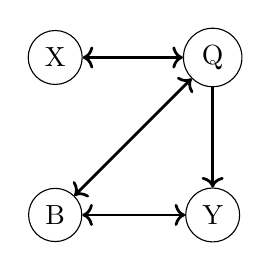
\begin{tikzpicture}
				\node[circle, draw] (X2) at (0, 0) {X};
				\node[circle, draw] (Q2) at (2, 0) {Q};
				\node[circle, draw] (B2) at (0, -2) {B};
				\node[circle, draw] (Y2) at (2, -2) {Y};
				\draw[<->, line width=1pt] (X2) -- (Q2);
				\draw[<->, line width=1pt] (Q2) -- (B2);
				\draw[<->, line width=1pt] (B2) -- (Y2);
				\draw[->, line width=1pt] (Q2) -- (Y2);
			\end{tikzpicture}
			\caption{MAG (i)}
			\label{fig:mag-csrc1}
		\end{figure}
	\end{minipage}
	
	\columnbreak
	
	\begin{minipage}{\linewidth}
		\begin{figure}[H]
			\centering
			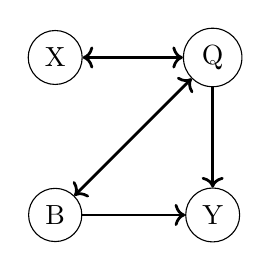
\begin{tikzpicture}
				\node[circle, draw] (X2) at (0, 0) {X};
				\node[circle, draw] (Q2) at (2, 0) {Q};
				\node[circle, draw] (B2) at (0, -2) {B};
				\node[circle, draw] (Y2) at (2, -2) {Y};
				\draw[<->, line width=1pt] (X2) -- (Q2);
				\draw[<->, line width=1pt] (Q2) -- (B2);
				\draw[->, line width=1pt] (B2) -- (Y2);
				\draw[->, line width=1pt] (Q2) -- (Y2);
			\end{tikzpicture}
			\caption{MAG (ii)}
			\label{fig:mag-csrc2}
		\end{figure}
	\end{minipage}
\end{multicols}
For example, the above MAGs are not Markov equivalent as the first one contains a discriminating path from $x$ to $y$ with $b \leftrightarrow y$ while the second the edge $b \rightarrow y$ which violates condition (iii). \\

The advantage of the constructive SRC is that it is not necessary to consider discriminating paths with non-colliders $b$; one only has to look for discriminating paths with a collider $b$. It also simplifies the notion of a discriminating path between $x$ and $y$: \textit{a collider path between non-adjacent endpoints} $x$ \textit{and} $y$ \textit{for which every vertex but the one before} $y$ \textit{is a parent of} $y$. This also results in the following reformulation for the Markov equivalence criterion on MAGs from Verma \& Pearl \cite{verma1990}:

\begin{corollary}[Corollary 4.3 in \cite{wienobst2022}]Two DAGs $\mathcal{G}_1$ and $\mathcal{G}_2$ are Markov equivalent iff
	\begin{enumerate}
		\item $\mathcal{G}_1$ and $\mathcal{G}_2$ have the same adjacencies,
		\item If in $\mathcal{G}_1$ there is an unshielded collider $x \rightarrow b \leftarrow y$ then $\mathcal{G}_2$ does not contain an edge $b \rightarrow y$ and vice-versa.
	\end{enumerate}
\end{corollary}

\begin{corollary}[Corollary 4.4 in \cite{wienobst2022}] Two DAGs $\mathcal{G}_1$ and $\mathcal{G}_2$ are Markov equivalent iff
	\begin{enumerate}
		\item $\mathcal{G}_1$ and $\mathcal{G}_2$ have the same adjacencies,
		\item if there is a collider path $(x,\ldots,b,y)$ between non-adjacent $x,y$ with every vertex but $x,b$ and $y$ being a parent of $y$ in $\mathcal{G}_1$, then $\mathcal{G}_2$ does not contain the edge $b \rightarrow y$ and vice-versa.
	\end{enumerate}
\end{corollary}

Algorithmically, the conditions (i) and (ii) in the constructive-SRC (Theorem \ref{thm:constr-src}) are checked in $\mathcal{O}(n^2)$ and $\mathcal{O}(n^3)$ time respectively. For condition (iii), one needs to check for each $b \leftrightarrow y$ in $\mathcal{G}_1$ for which $b \rightarrow y$ is an edge in $\mathcal{G}_2$, whether there is a discriminating path for $b$ and $y$ (and vice-versa). This is done by considering every choice of $y$ consecutively and computing for each the \textit{bidirected connected components of its parents (called the parent districts)}:

\begin{definition}[Parent districts]For a MAG $\mathcal{G} = (\mathcal{V},\mathcal{E})$ and a vertex $y$, the bidirected connected components of $\mathcal{G}[\text{Pa}(y)]$ are called the \textbf{parent discricts of} $\mathbf{y}$, denoted $\mathcal{D}(y)$.
\end{definition} 

The algorithmic analysis of algorithm \ref{alg:wienobst} is the following: The conditions (i) and (ii) in the constructive-SRC (Theorem \ref{thm:constr-src}) are checked in $\mathcal{O}(n^2)$ and $\mathcal{O}(n^3)$ time respectively in line 1 (In fact checking unshielded colliders is $\Omega(n^3)$ so we cannot achieve complexity better than $\mathcal{O}(n^3)$ already). The loop at line 4 is $\mathcal{O}(n)$ as there are $n$ vertices to run through, while computing the parent districts (bidirected connected components) for a single $y$ can be done in $\mathcal{O}(n+e)$ using Tarjan's algorithm. The loop at line $8$ over $b$ is at worst $\mathcal{O}(n)$, and checking whether $b \rightarrow y$ exists in the other graph is constant $\mathcal{O}(1)$. Hence in total $\mathcal{O}(n^3)$. 


%\begin{algorithm}
%	\caption{Generate Random ADMG}
%	\label{alg:wienobst2}
%	\begin{algorithmic}[1]
%		\renewcommand{\algorithmicrequire}{\textbf{Input:}}
%		\renewcommand{\algorithmicensure}{\textbf{Output:}}
%		\Require $n, e = f(n)$
%		\Ensure A random ADMG
%		
%		\For{$i \leftarrow 1$ to $n$}
%		\State Fix a topological ordering on vertex $i$
%		\EndFor
		
%		\State $edge\_count \leftarrow 0$
		
%		\While{$\text{edge\_count} < e \times n$}
%		\State Randomly select two vertices $u, v \in V$
%		\State Ensure $u \leq v$
		
%		\If{$u \neq v$ and not $u \rightarrow v$ and not $u \leftrightarrow v$}
%		\State Sample $p \sim \mathcal{U}(0,1)$
%		\If{$p < 0.5$}
%		\State Add a directed edge $u \rightarrow v$
%		\Else
%		\State Add a bidirected edge $u \leftrightarrow v$
%		\EndIf
%		\State $\text{edge\_count} \leftarrow \text{edge\_count} + 1$
%		\EndIf
%		\EndWhile
%		
%	\end{algorithmic}
%\end{algorithm}

\section{Experiments}

\subsection{Implementation and setup}

All three algorithms are implemented in the Julia programming language \cite{julia2012} relying on and enhancing the implementation of \cite{wienobst2022}. The reasons are plenty: Julia combines both high-level expressiveness and low-level performance capabilities. Also, graph manipulation is highly convenient using the Graphs library with preimplemented methods such as connected components using Tarjan's algorithm. The language's support for Unicode characters (such as set operations on set objects) enhances code readability when translating graph algorithms from pseudocode to Julia. Julia's native multi-threading capabilities also contribute to improved runtime performance. 

The experiments are carried out as follows: Acyclic Directed Mixed Graphs (ADMGs) are generated for varying number of nodes and edges using modified random DAG generators to also introduce bidirected edges. More specifically, modified Erd\H{o}s-R\'{e}nyi random DAGs \cite{erdos1959} and Barab\'{a}si-Albert models \cite{barabasi1999} to generate ADMGs instead of DAGs, which are then converted into MAGs. (More random DAG algorithms could have been implemented, such as Watts-Strogatz, Geometric random graphs or complete bipartite graphs but the time complexity for each configuration would raise massively, maybe in a future contribution).
% and the method implemented by Hu and Evans \cite{hu2020}: Given a number $n$ of vertices and $e$ of edges, fix a topological ordering of the vertices. Then two vertices become adjacent  with uniform probability. Once this skeleton construction phase is determined, an edge is independently either directed or bidirected equiprobably. 

In the Erd\H{o}s-R\'{e}nyi DAG model, we initialize $n$ vertices with no edges. We then fix a topological ordering of the vertices, and generate fixed number of edges $(e=dn$ where $d$ is the average degree, a modification on the original $\mathcal{G}_{n,p}$ directed random graph) with the following rule: For each pair of vertices  $v$ and $u$ in the graph ($v \neq u$) independently add a directed edge from $v$ to $u$ with probability $p$. If cycles occur, remove edges to ensure the graph is acyclic. Our modification is to also either add a directed edge from $v$ to $u$ with probability $p$ or a bidirected edge with probability $1-p$ and again check for almost directed cycles - that is, bidirected cycles (recall definition of ancestrality), see Algorithm \ref{alg:erdos-renyi-admg}.

\begin{algorithm}
	\caption{Erdős-Rényi MAG generator}
	\label{alg:erdos-renyi-admg}
	\begin{algorithmic}[1]
		\renewcommand{\algorithmicrequire}{\textbf{Input:}}
		\renewcommand{\algorithmicensure}{\textbf{Output:}}
		\Require $n$, $p$, $d$
		\Ensure  a MAG $G$
		\State initialize $G$ as an empty directed graph with $n$ nodes
		\For{$i \leftarrow 1$ to $n$}
			\State Fix a topological ordering on vertex $i$
			\EndFor
		\State initialize $edges$ with all possible directed arcs in $G$
		\While {number of edges in $G \leq dn$}
		\State $e \leftarrow$ pop(shuffle($edges$))
		\If {$p \leq$ random uniform sample in $[0,1]$}
		\State $G^{'} \leftarrow G$ \Comment{Make a copy of G}
		\State add directed edge $e$ to $G^{'}$
		\Else
		\State $G^{'} \leftarrow G$ \Comment{Make a copy of G}
		\State add bidirected edge $e$ to $G^{'}$
		\EndIf
		\If {$G^{'}$ has no directed cycles or almost directed cycles}
		\State $G \leftarrow G^{'}$ \Comment{Update G with the new edge}
		\EndIf
		\EndWhile
		\State $G \leftarrow \text{ADMG\_to\_MAG}(G)$
		\State \Return $G$ 
	\end{algorithmic} 
\end{algorithm}

In the Barab\'{a}si-Albert model, a graph of $n$ nodes is grown by attaching new nodes each with $m$ edges preferentially to nodes with high degree. $n$ nodes. We first start with a small set of nodes ($m=3$) that represents a cluster connected a star graph. Then we add nodes one at a time till we obtain $n$ nodes. When we add a node, we connect it to a small number of existing nodes with probability proportional to the degree of the existing node. As a result, nodes with higher degree (the ones in the earlier iterations) tend to get even higher degree (rich-get-richer effect). The name "scale-free" network stems that the degree distribution is power-law, $P(k) \sim k^{-\gamma}$ where $2 < \gamma < 3$ ($P(k)$ is the ratio of nodes with degree k to the total number of nodes). The second moment of the distribution (scale) is infinite, hence the name scale-free. In this case, we employ the same rationale as in Erd\H{o}s-R\'{e}nyi DAGs, where the connected graph is generated with directed edges. We then randomly choose two vertices and add bidirected edges until their sum to a predefined quantity ($e=dn$) with probability $p$, that is, we also introduce the a probability parameter $p$ to the model. The parameter $0 < p < 1$ is set from $p \in \left\{ 0.2, 0.5, 0.8 \right\}$; a low value of $p$ over $1-p$ favors the insertion of bidirected edges. In this case, the degree distribution of bidirectional edges does not follow a power-law like in the DAG case of an Erd\H{o}s-R\'{e}nyi scale-free graph (which can also be modified), see Algorithm \ref{alg:barabasi-albert-admg}. 

\begin{algorithm}
	\caption{Barabási-Albert random MAG generator}
	\label{alg:barabasi-albert-admg}
	\begin{algorithmic}[1]
		\renewcommand{\algorithmicrequire}{\textbf{Input:}}
		\renewcommand{\algorithmicensure}{\textbf{Output:}}
		\Require $n$, $m$, $m_0$, $d$, $p$
		\Ensure a MAG $G$
		\For{$i \leftarrow 1$ to $n$}
		\State Fix a topological ordering on vertex $i$
		\EndFor
		\State $G = (V_G, E_G) $ a random star graph with $m_0$ nodes
		\State $G \leftarrow$ ToDag$(G)$ \Comment{Convert the graph to a DAG}
		\State $rp \leftarrow [ \ ]$ \Comment{List of potential attachment points}
		\For{$v$ in $V_G$}
		\State append $v$ to $rp$ as many times as its degree in $G$
		\EndFor
		\While{$|E_G| \leq dn$}
		\State $targets \leftarrow$ RandomSubset($rp$, $n$)
		\State $t_1 \leftarrow$ RandomNode($V_G$)
		\For{$t_2$ in $targets$}
		\If{$p \leq$ random uniform sample in $[0,1]$}
		\State $E_G \leftarrow E_G \cup (t_1, t_2)$
		\Else
		\If{graph $(V_G, E_G \cup (t_1, t_2))$ is almost acyclic}
		\State $E_G \leftarrow E_G \cup (t_1 \leftrightarrow t_2)$
		\EndIf
		\EndIf
		\EndFor
		\State append $targets$ to $rp$
		\State append $t_1$ to $rp$ $m$ times
		\EndWhile
		\State $G \leftarrow \text{ADMG\_to\_MAG}(G)$
		\State \Return $G$ 
	\end{algorithmic} 
\end{algorithm}

The generated AMDGs are then converted to MAGs using the AG projection algorithm by Hu and Evans (Algorithm \ref{alg:admg-mag}). During the conversion, we keep track of the amount of directed and bidirected edges. For each configuration, 100 MAGs are generated to obtain a mean empirical execution time and variance, and 10 MAGs for dense graphs due to very high running time. Since causal graphs are in general sparse, we are testing with degree up to a total of $30n$ number of edges ($d=30$). The combinations for vertices and edges ($e=dn$)are the following:  $d \in \left\{1,3,5,10,15,30 \right\}$. For $d=1$, we generate graphs from $5$ to $2 \cdot 10^3$ vertices, for $d=3$ from $10$ to $10^3$, for $d=5$ from $25$ to $10^3$, for $d=10$ from $30$ to $500$ and for $d=15$ and $30$ from $100$ to $500$.

To ease the implementation, we split each algorithm in a separate Julia module (\texttt{asr.jl},~\texttt{hu.jl},~\texttt{csrc.jl}), a helper module containing various utility functions for Graph manipulation (\texttt{Graph\_utils.jl}) and our random graph generation algorithms (\texttt{Graph\_generators.jl}). We use a plethora of Julia libraries, particularly \texttt{Graphs} (for graph handling and manipulation, as well as pre-implemented algorithms such as connected components), \texttt{DataStructures} (for stack, queue and set objects when implementing the algorithms), \texttt{Random} and \texttt{Statistics} (for probability distributions, generators and sampling), \texttt{ProgressBars} (for dynamically tracking the progress of the experiments on screen) and \texttt{Dates} (for handling execution time and logging). We represent Maximal Ancestral Graphs as a \textit{pair of two graphs with the same vertices}, one with \textit{directed edges} and one with \textit{undirected edges} (that represent the bidirected edges). In order to run the experiments, one simply executes \texttt{julia experiments.jl}, with the results available in a dedicated logs folder. Due to computational complexity, the experiments are run locally on an AMD Ryzen Threadripper 16-core workstation for several weeks, with 128GB of memory. Visualization on the terminal window regarding the progress of the experiments is done using the \texttt{tqdm} library. For an illustration of the running script see Figure \ref{fig:tqdm} in the Appendix. Complete code is available\footnote{\url{https://github.com/kougioulis/CS-583}.}

\begin{figure}[htbp]
	\centering
	\subfigure[Plot 1]{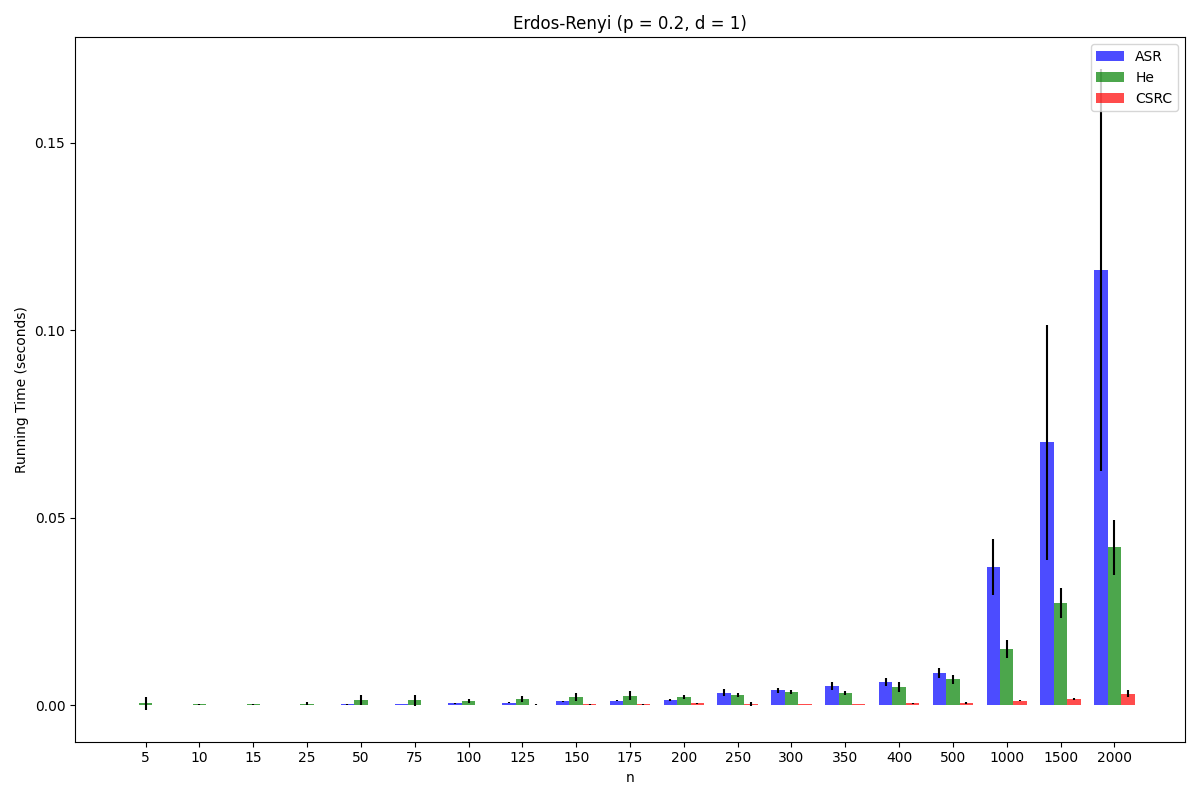
\includegraphics[width=0.49\textwidth]{figures/Figure_1.png}}
	\hfill
	\subfigure[Plot 2]{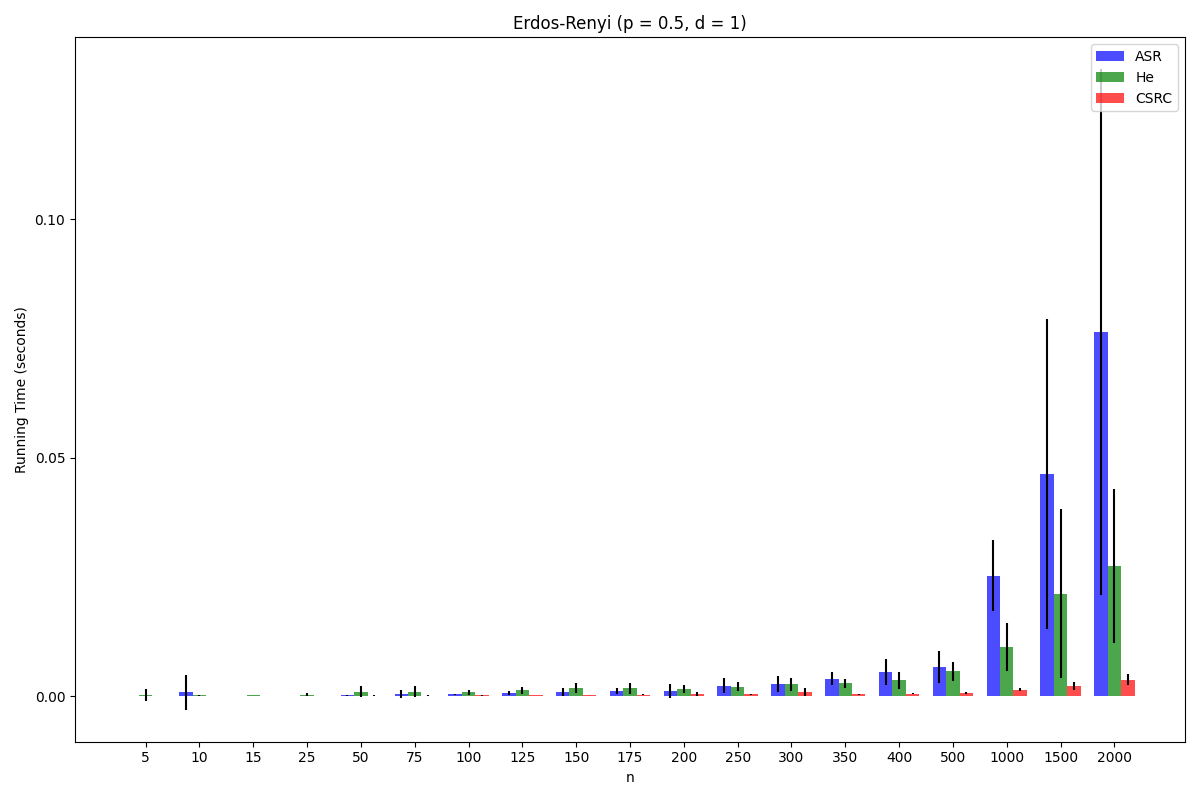
\includegraphics[width=0.49\textwidth]{figures/Figure_2.png}}
	
	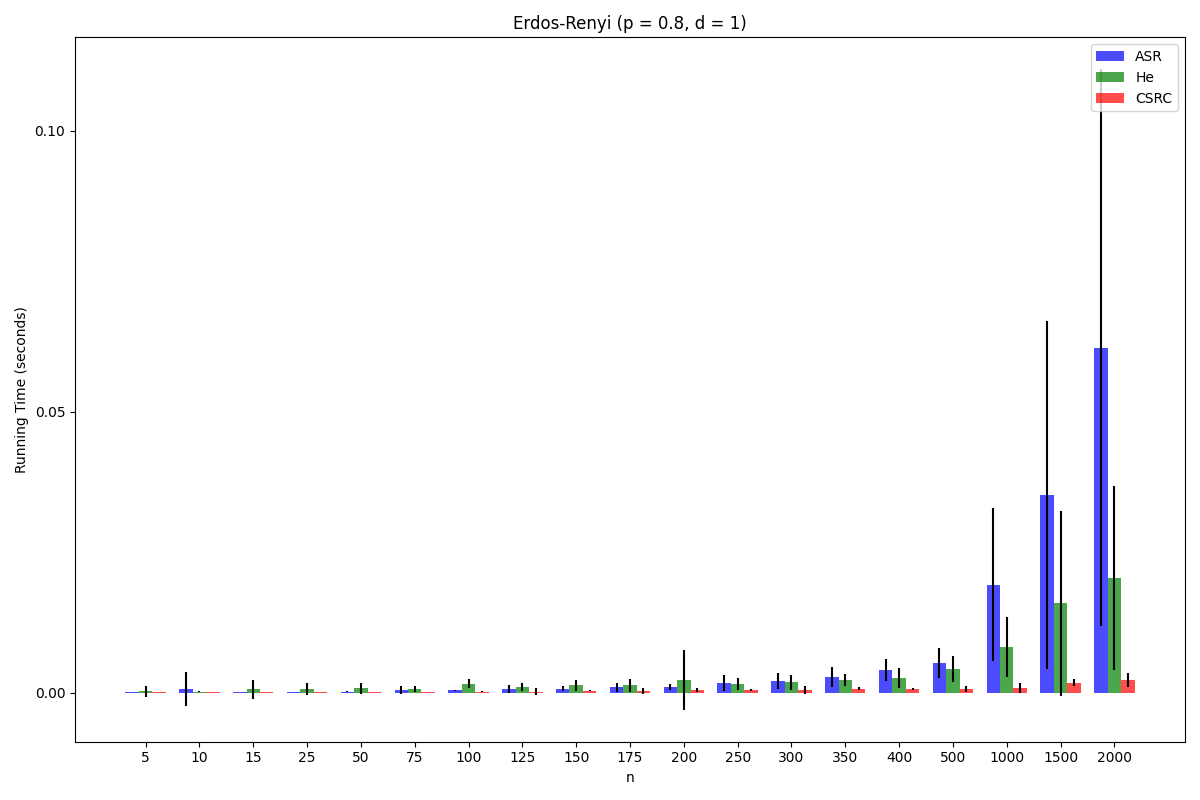
\includegraphics[width=0.49\textwidth]{figures/Figure_3.png}
	
	\caption{Running time plots for each algorithm (Ali-Spirtes-Richardson (ASR) in blue, Hu-Evans (He) in green and Constructive-SRC (CSRC) in red) for sparse Erd\H{o}s-R\'{e}nyi MAGs ($d=1$) and $p=0.2$~(Figure (a)), $p=0.5$~(Figure (b)), $p=0.8$~(Figure (c)).}
	\label{fig:er-1}
\end{figure}

\subsection{Experimental Results}

\subsubsection{Modified Erd\H{o}s-R\'{e}nyi model}

In the following pages, we report the average running times and standard deviations of each configuration for MAGs based on the Erd\H{o}s-R\'{e}nyi model. We illustrate the plots for sparse graphs ($d=1$) and dense graphs ($d=30$). All plots for $d=1,3,5,15,30$ are available in the appendix. 

In the Erd\H{o}s-R\'{e}nyi model, big differences are observed in running time even for very sparse graphs between the three algorithms, and even more prominently for dense graphs. We notice that for larger values of $p$, the average running times are lower for all algorithms as well as their standard deviation (a value of $p$ close to $1$ will highly favor directed over bidirected edges). That is, the more latent confounders are assumed to exist between variables, the higher the running complexity.


\begin{figure}[htbp]
	\centering
	\subfigure[Plot 1]{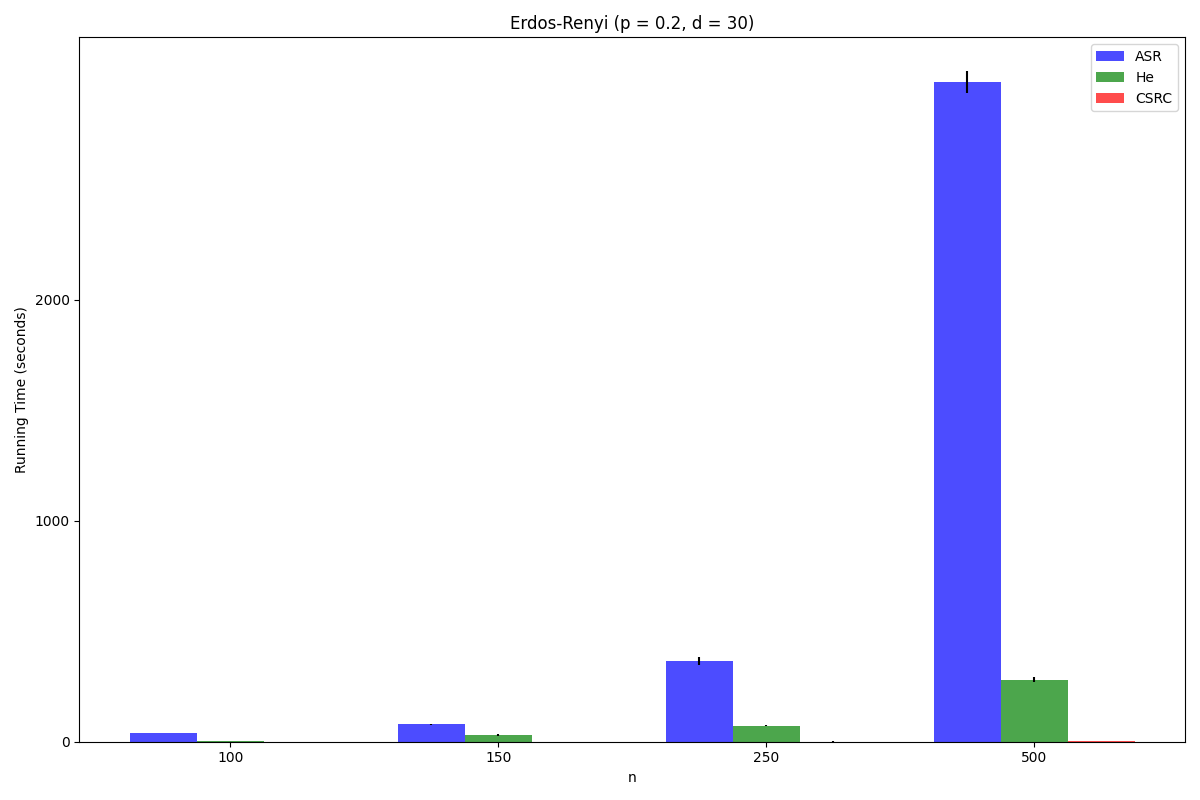
\includegraphics[width=0.49\textwidth]{figures/Figure_13.png}}
	\hfill
	\subfigure[Plot 2]{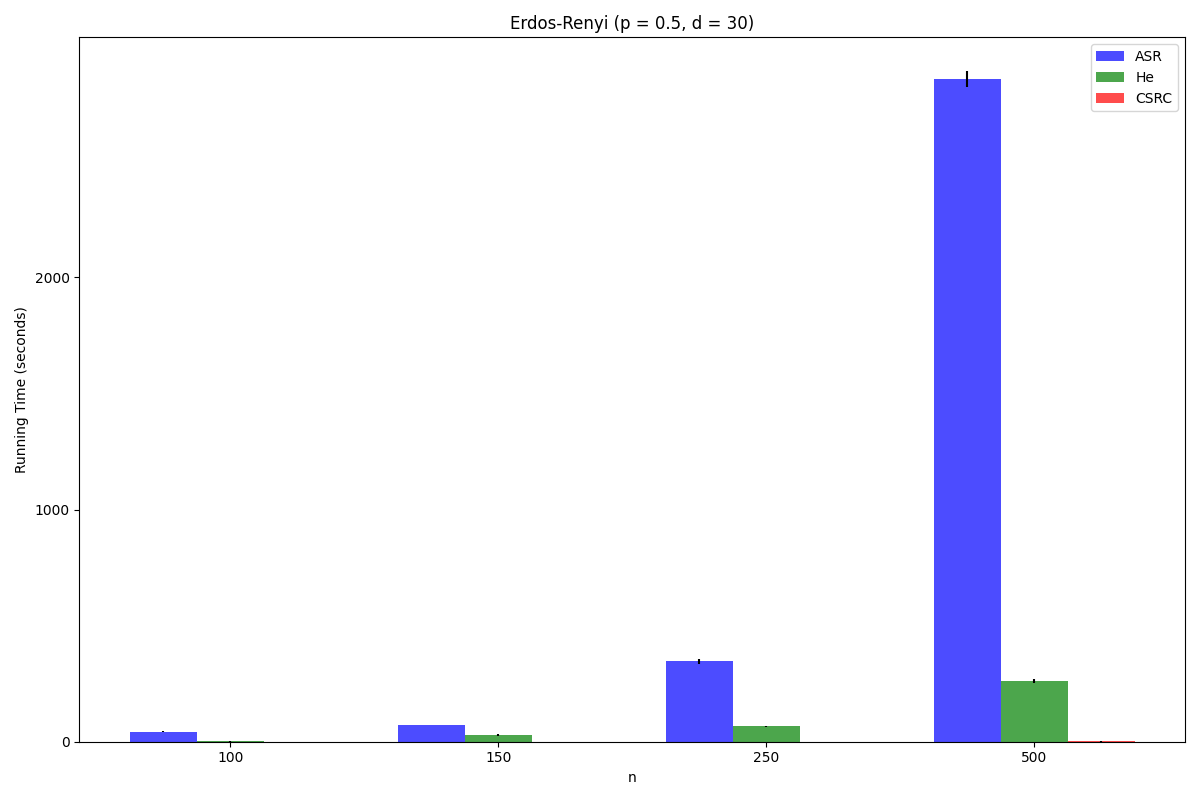
\includegraphics[width=0.49\textwidth]{figures/Figure_14.png}}
	
	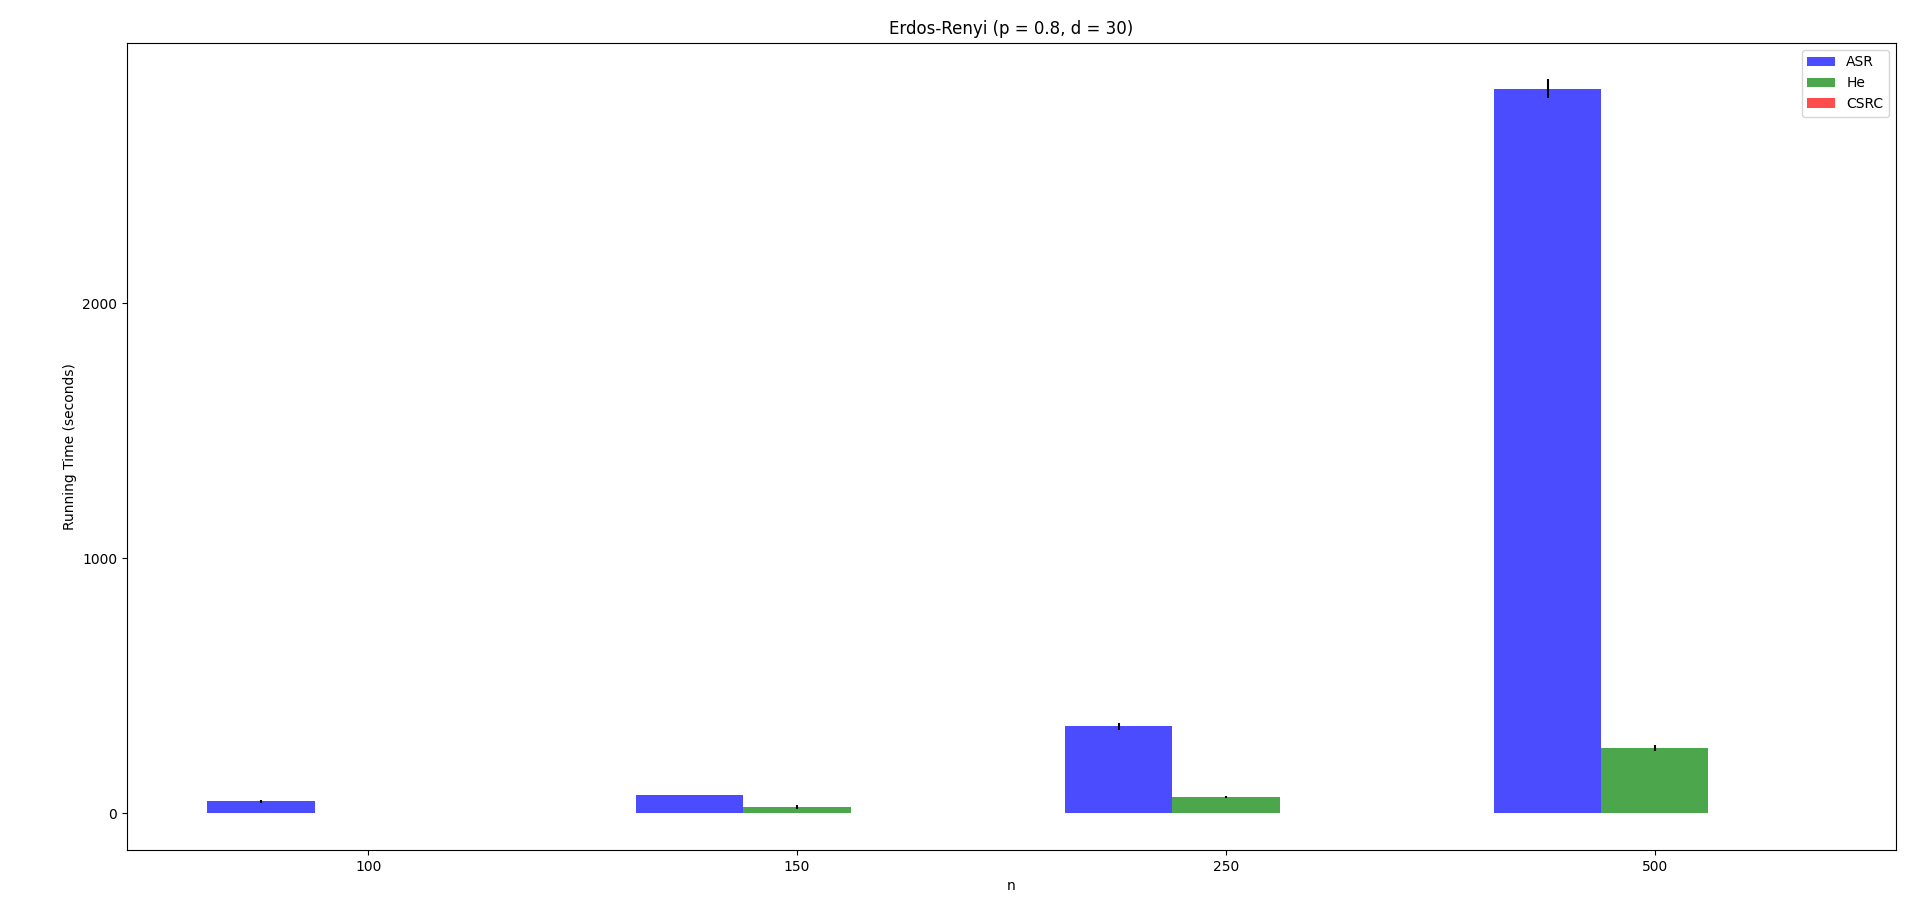
\includegraphics[width=0.52\textwidth]{figures/Figure_15.png}
	
	\caption{Running time plots for each algorithm (Ali-Spirtes-Richardson (ASR) in blue, Hu-Evans (He) in green and Constructive-SRC (CSRC) in red) for dense Erd\H{o}s-R\'{e}nyi MAGs ($d=30$) and $p=0.2$~(Figure (a)), $p=0.5$~(Figure (b)), $p=0.8$~(Figure (c)).}
	\label{fig:er-30}
\end{figure}

\pagebreak

\subsubsection{Modified Barab\'{a}si-Albert model}

\begin{figure}[htbp]
	\centering
	\subfigure[Plot 1]{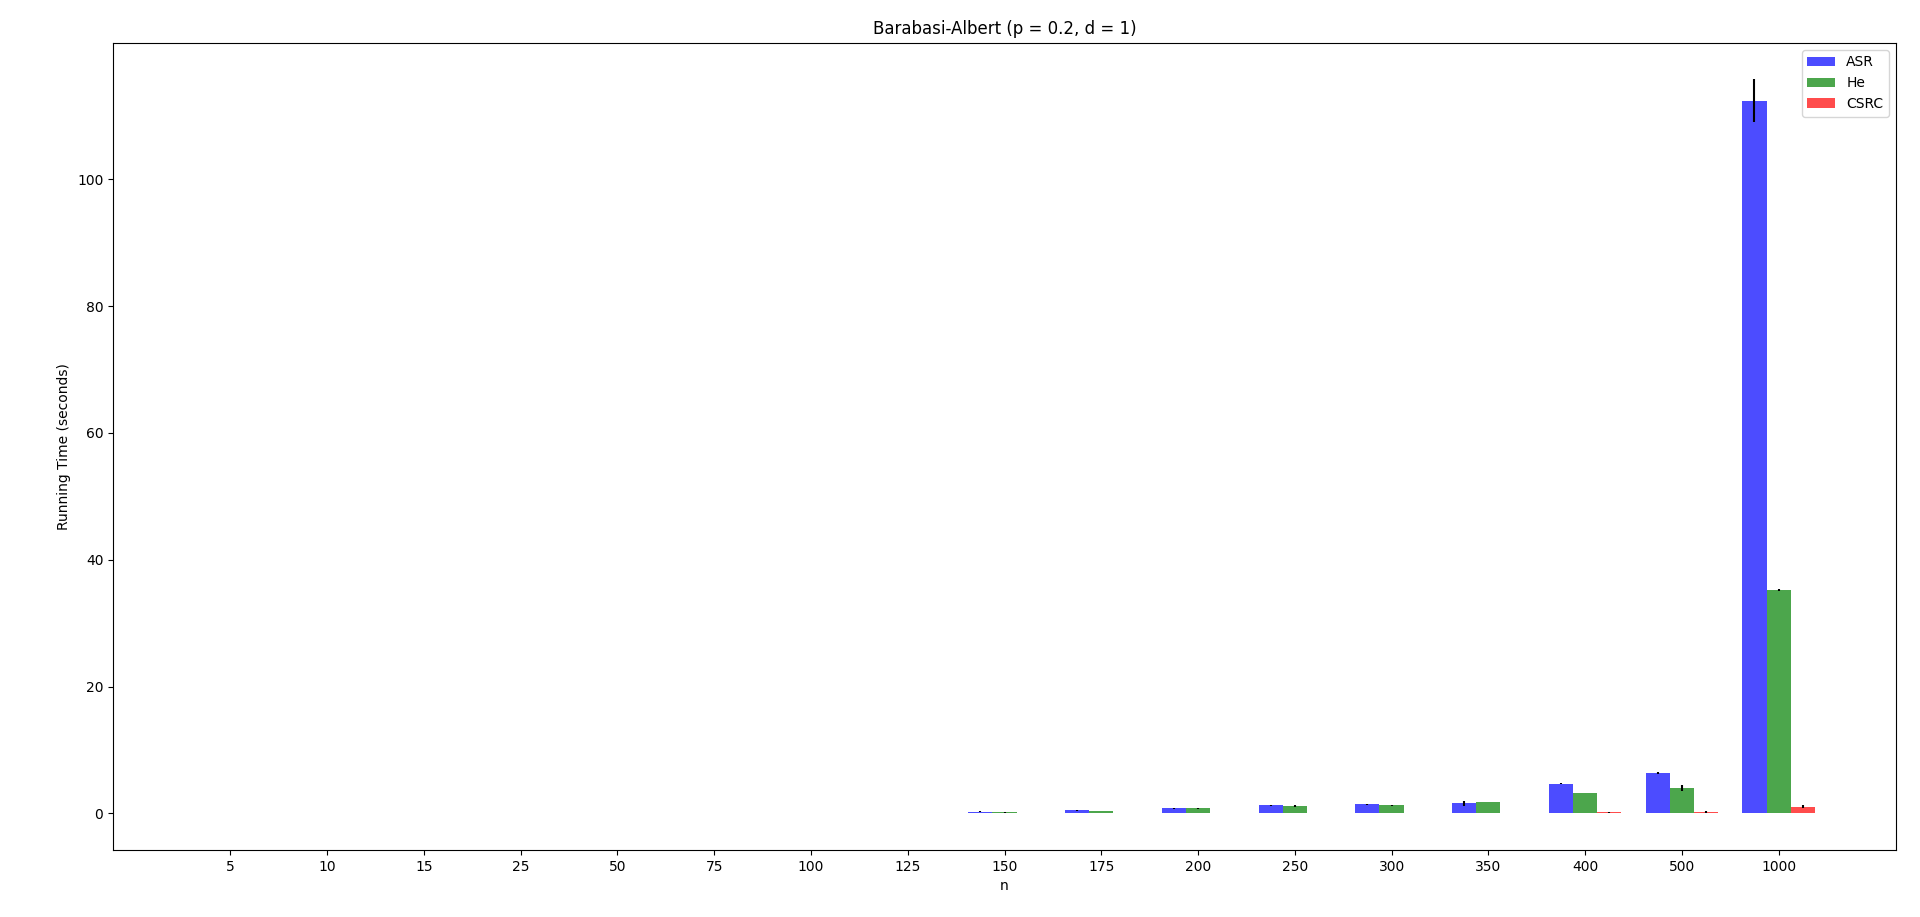
\includegraphics[width=0.49\textwidth]{figures/Figure_16.png}}
	\hfill
	\subfigure[Plot 2]{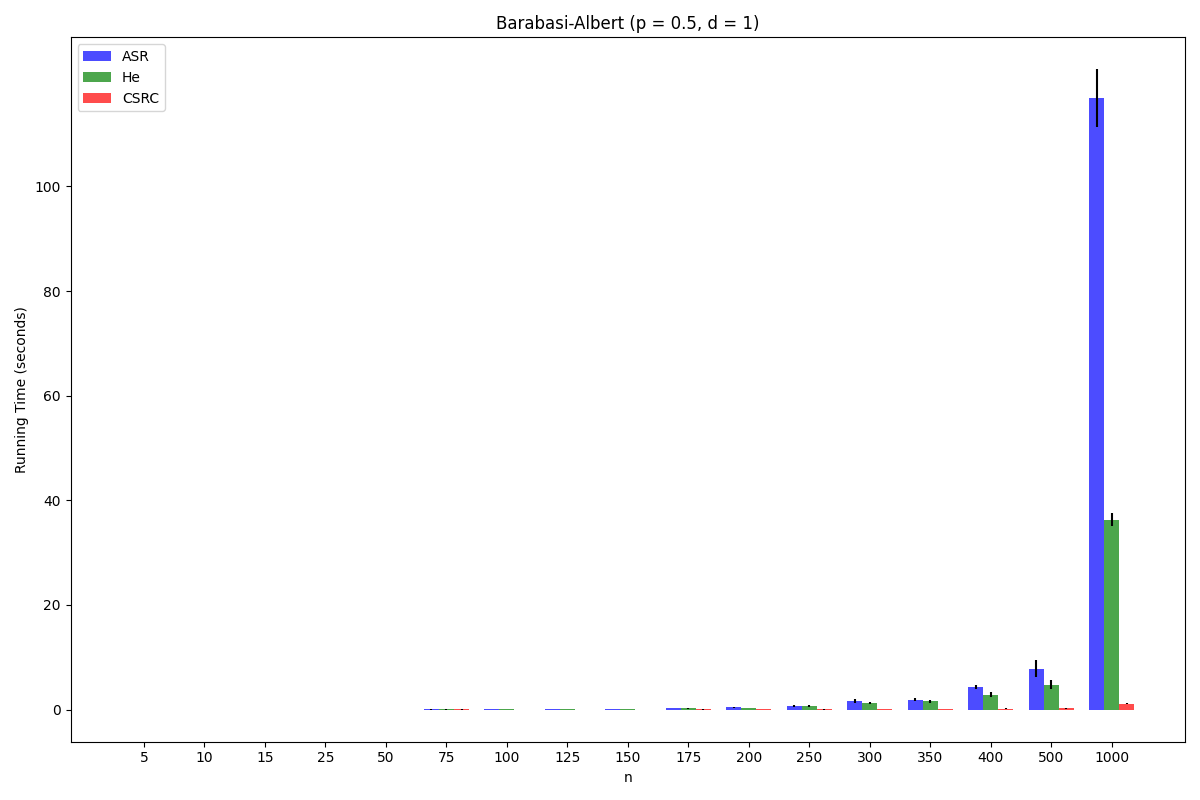
\includegraphics[width=0.49\textwidth]{figures/Figure_17.png}}
	
	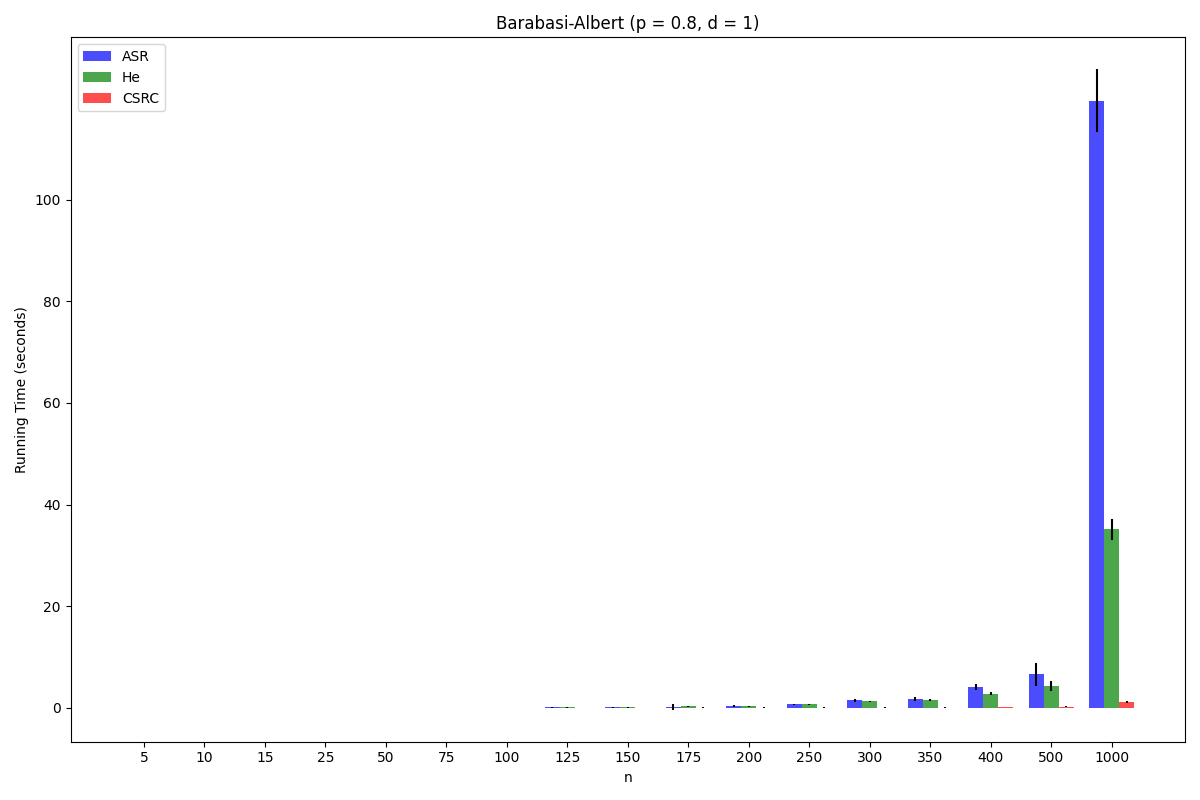
\includegraphics[width=0.52\textwidth]{figures/Figure_18.png}
	
	\caption{Running time plots for each algorithm (Ali-Spirtes-Richardson (ASR) in blue, Hu-Evans (He) in green and Constructive-SRC (CSRC) in red) for sparse Barabasi-Albert MAGs ($d=1$) and $p=0.2$~(Figure (a)), $p=0.5$~(Figure (b)), $p=0.8$~(Figure (c)).}
	\label{fig:sf-1}
\end{figure}

Regarding MAGs based on scale-free graphs using the Barab\'{a}si-Albert model, very similar characteristics are observed between the algorithms like in the Erd\H{o}s-R\'{e}nyi model. The running times are much higher, especially for the Ali-Spirtes-Richardson and Hu-Evans algorithms, due to the rich-get richer effect concentrating a high amount of edges in clusters.

\begin{figure}[htbp]
	\centering
	\subfigure[Plot 1]{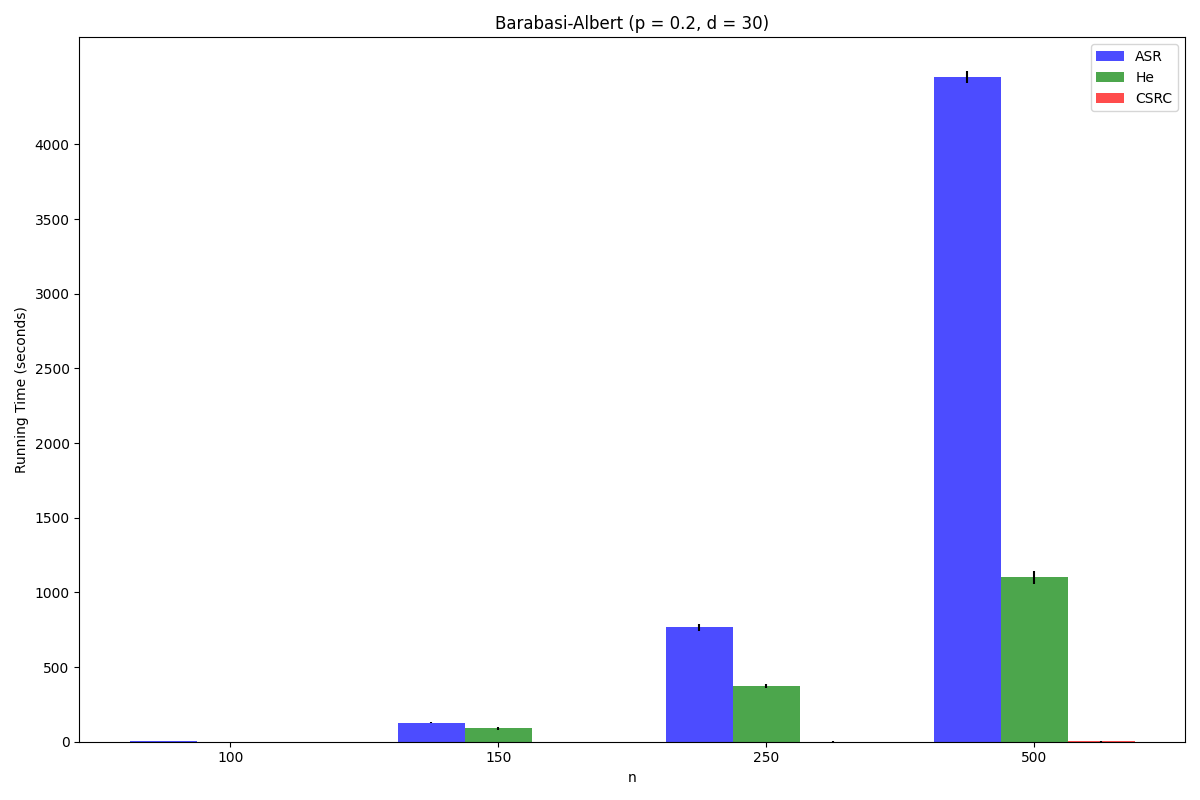
\includegraphics[width=0.49\textwidth]{figures/Figure_25.png}}
	\hfill
	\subfigure[Plot 2]{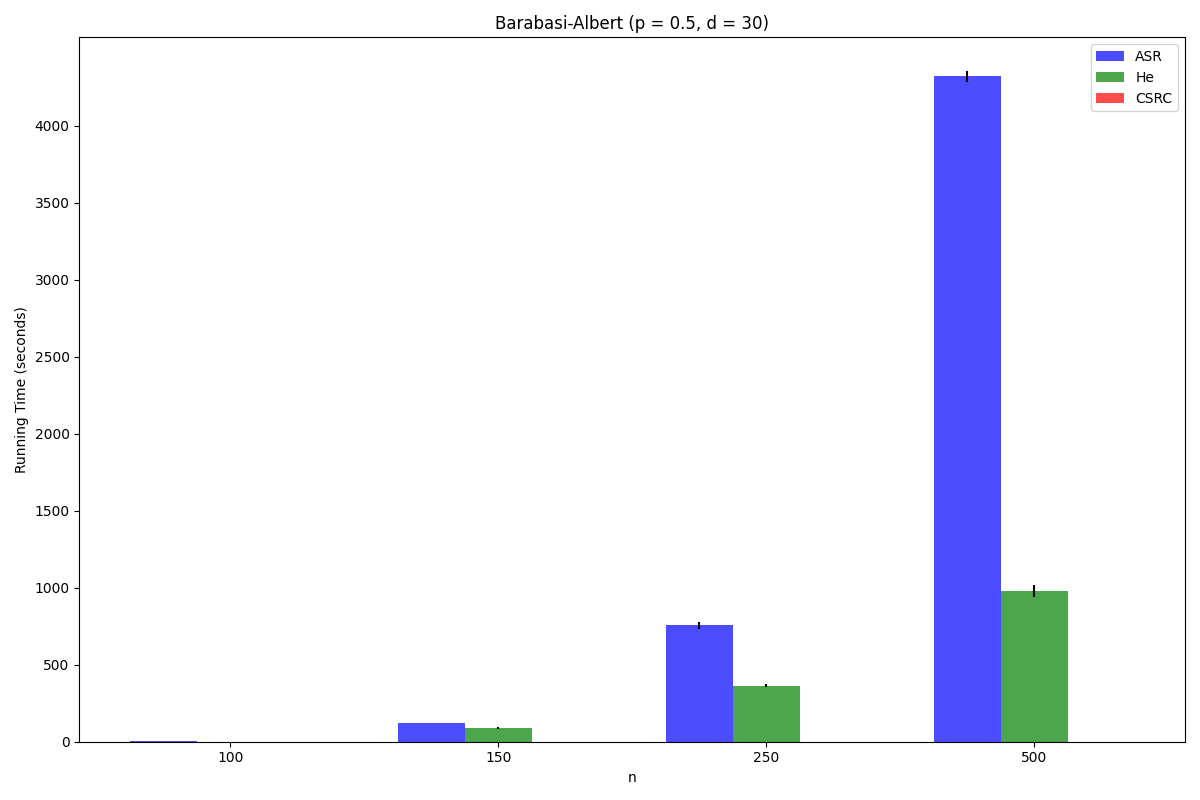
\includegraphics[width=0.49\textwidth]{figures/Figure_26.png}}
	
	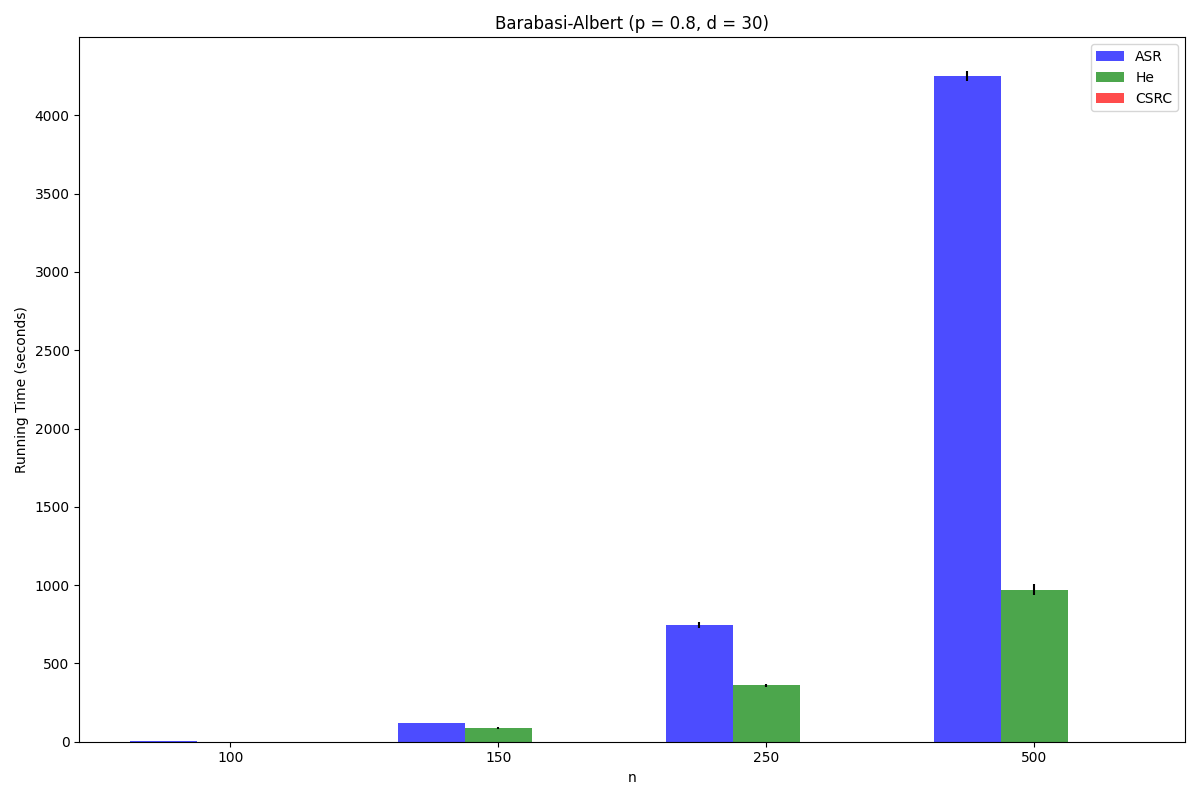
\includegraphics[width=0.49\textwidth]{figures/Figure_27.png}
	
	\caption{Running time plots for each algorithm (Ali-Spirtes-Richardson (ASR) in blue, Hu-Evans (He) in green and Constructive-SRC (CSRC) in red) for dense Barabasi-Albert MAGs ($d=30$) and $p=0.2$~(Figure (a)), $p=0.5$~(Figure (b)), $p=0.8$~(Figure (c)).}
	\label{fig:sf-30}
\end{figure}
\pagebreak
\subsection{Conclusion}

We have presented maximal ancestral graphs (MAGs), a class of graphical models viewed as an extension to causal DAGs that drop the causal sufficiency condition and are able to model latent confounders and selection bias. When learning MAGs from observational data, like DAGs, multiple MAGs may encode the same statistical (in)dependencies. Such MAGs are called Markov equivalent. Is it of importance in the field of causal discovery to test whether two MAGs are Markov equivalent. Although checking Markov equivalence in DAGs is  straightforward, this is not transferred directly to MAGs. Over the years three algorithms have been developed using the Spirtes-Richardson criterion to check for Markov equivalence. The Ali-Spirtes-Richardson algorithm works by constructing triples in order in a recursive manner, level-by-level. The Hu-Evans algorithm constructs the so-called parametrizing sets of a MAG and checks for Markov-equivalence if both MAGs have the same parametrizing sets. The Wienbost-Bannach algorithm, called Constructive-SRC, is a constructive method based on the Spirtes-Richardson criterion using the parent districts of the vertices. We modify known random DAG generators to generate ADMGs and then convert them to MAGs, called modified Erd\H{o}s-R\'{e}nyi and modified Barabasi-Albert MAG generators and set up experiments in the Julia programming language. For sparse graphs, which are prominent in causal discovery, the Ali-Spirtes-Richardson and Hu-Evans algorithms have similar performance. On denser graphs, where the running time of the first two algorithms is much higher than in smaller graphs, the performance advantage of the constructive-SRC algorithm is highly prominent. Very similar but amplified results are shown in Barabasi-Albert graphs, due to their structure. More results can be obtained for other types of graphs, such as geometric random and bipartite random graphs. 

As a final note, causal discovery libraries such as \texttt{causaldag} implement Markov equivalence on MAGs using the Ali-Spirtes-Richardson algorithm\footnote{\url{https://causaldag.readthedocs.io/en/latest/classes/generated/causaldag.classes.ancestral\_graph.AncestralGraph.markov\_equivalent.html}.}. We are looking forward to implement the faster algorithms of Hu-Evans and Wienbost-Bannach-Liskiwicz to the package.

\pagebreak

\begin{thebibliography}{}
	\bibitem{pearl2009} Pearl, J. (2009). \textit{Causality.} Cambridge University Press.
	\bibitem{spirtes2000} Spirtes, P., Glymour, C. N., \& Scheines, R. (2000). \textit{Causation, Prediction, and Search.} MIT press.
	\bibitem{richardson2002} Richardson, T., \& Spirtes, P. (2002). \textit{Ancestral graph Markov models.} The Annals of Statistics, 30(4), 962.
	\bibitem{verma1990} Verma, T., \& Pearl, J. (1990). \textit{Equivalence and Synthesis of Causal Models.} In Proceedings of the Sixth Annual Conference on Uncertainty in Artificial Intelligence (pp. 255-270).
	\bibitem{spirtes1996} Spirtes, P., \& Richardson, T. (1996). \textit{A polynomial time algorithm for determining DAG equivalence in the presence of latent variables and selection bias.} In Proceedings of the 6th International Workshop on Artificial Intelligence and Statistics (pp. 489-500).
	\bibitem{ali2009}R Ayesha Ali, Richardson T., \& Spirtes, P. (2009). \textit{Markov equivalence for Ancestral Graphs.} The Annals of Statistics, 37(5B):2808–2837.
	\bibitem{hu2020} Hu, Z., \& Evans, R. (2020). \textit{Faster algorithms for Markov Equivalence.} In Conference on Uncertainty in Artificial Intelligence (pp. 739-748). PMLR.
	\bibitem{wienobst2022} Wienöbst, M., Bannach, M., \& Liśkiewicz, M. (2022). \textit{A new constructive criterion for Markov equivalence of MAGs}. In Uncertainty in Artificial Intelligence (pp. 2107-2116). PMLR.
	\bibitem{erdos1959} Erd\H{o}s, P., \& R\'{e}nyi, A. (1959). \textit{On random graphs I}. Publ. Math. debrecen, 6(290-297), 18.
	\bibitem{barabasi1999} Barabási, A. L., \& Albert, R. (1999). \textit{Emergence of scaling in random networks}. Science, 286(5439), 509-512.
	
	\bibitem{julia2012} Bezanson, J., Karpinski, S., Shah, V. B., \& Edelman, A. (2012). \textit{Julia: A fast dynamic language for technical computing}. arXiv preprint arXiv:1209.5145.
\end{thebibliography}

\newpage

\appendix

\section{Appendix}

\subsection{Ali-Spirtes-Richardson Algorithm}

\begin{algorithm}
	\caption{The algorithm $\text{Reachable}(\mathbb{D},\mathbf{w})$}
	\label{alg:asr-reachable}
	\begin{algorithmic}[1]
		\renewcommand{\algorithmicrequire}{\textbf{Input:}}
		\renewcommand{\algorithmicensure}{\textbf{Output:}}
		\Require A directed graph $\mathbb{D}(\mathbb{V}, \mathbb{E})$; an element $\mathbf{w} \in \mathbb{V}$
		\Ensure A set $\mathbb{S}$ of elements connected to $\mathbf{w}$ in $\mathbb{D}$
		
		\State $\mathbb{S}_0 = \emptyset$; $\mathbb{S}_1 = \{\mathbf{w}\}$; $p = 1$
		
		\Repeat
		\State $\mathbb{S}_{p+1} = \mathbb{S}_p \cup \{\mathbf{w}_2 \mid \mathbf{w}_1 \in \mathbb{S}_p \setminus \mathbb{S}_{p-1} \text{ and } (\mathbf{w}_1, \mathbf{w}_2) \in \mathbb{E}\}$
		\State $p = p + 1$
		\Until{$\mathbb{S}_p = \mathbb{S}_{p-1}$}
		
		\Return $\mathbb{S} = \mathbb{S}_p$
	\end{algorithmic}
\end{algorithm}

\begin{algorithm}
	\caption{Triples($\mathcal{G}$)}
	\label{alg:asr-triples}
	\begin{algorithmic}[1]
		\renewcommand{\algorithmicrequire}{\textbf{Input:}}
		\renewcommand{\algorithmicensure}{\textbf{Output:}}
		\Require A MAG $\mathcal{G}$
		\Ensure set of triples $T$ such that $\text{OCol}(\mathcal{G}) \subseteq T \subseteq \text{ICol}(\mathcal{G})$
		
		\State $T_0 = \{(a, b, c) \mid (a, b, c) \in \text{Col}(\mathcal{G}), (a, c) \notin \text{Adj}(\mathcal{G})\}$
		\State $k = 0$
		
		\Repeat $~k = k + 1$
		
		$T_k = T_{k-1}$
		
		\For{each $(a, b, c) \in \text{Col}(\mathcal{G}) \setminus T_{k-1}$ with $a \in \text{sp}_\mathcal{G}(b) \cap \text{pa}_\mathcal{G}(c)$}
		\State $V = \{(t, u) \mid t, u \in \text{pa}(c), t \leftrightarrow u \text{ in } G\} \cup \{(b, a)\}$
		
		\State $E = \{((t, u), (u, v) \mid (t, u, v)) \in T_{k-1}, (t, u), (u, v) \in V\}$
		\State $S = \text{Reachable}((V, E), (b, a))$
		\State $X = \{x \mid \exists ~y, z, (z, y, x) \in T_{k-1}, (z, y) \in S\}$
		
		\If{$X \setminus \{v \mid (v, c) \in \text{Adj}(G)\} \neq \emptyset$}
		$T_k = T_k \cup \{(a, b, c), (c, b, a)\}$
		\EndIf
		\EndFor
		
		\Until{$T_k = T_{k-1}$}
		
		\Return $T = T_k$
	\end{algorithmic}
\end{algorithm}

\begin{algorithm}
\caption{Equivalent}
\label{alg:asr-equiv}
\begin{algorithmic}[1]
	\renewcommand{\algorithmicrequire}{\textbf{Input:}}
	\renewcommand{\algorithmicensure}{\textbf{Output:}}
	\Require Two maximal ancestral graphs $\mathcal{G}_1$ and $\mathcal{G}_2$
	\Ensure A Boolean variable indicating whether $\text{I}_m(\mathcal{G}_1) = \text{I}_m(\mathcal{G}_2)$ (That is, being the same I-map, which is entailing the same m-separation properties, which is being Markov equivalent \cite{pearl2009}).
	
	\If{$\text{Adj}(\mathcal{G}_1) \neq \text{Adj}(\mathcal{G}_2)$}
	\Return False
	\EndIf
	
	\If{$\text{Triples}(\mathcal{G}_1) \setminus \text{Col}(\mathcal{G}_2) \neq \emptyset$}
	\Return False
	\EndIf
	
	\If{$\text{Triples}(\mathcal{G}_2) \setminus \text{Col}(\mathcal{G}_1) \neq \emptyset$}
	\Return False
	\EndIf
	
	\Return True
\end{algorithmic}
\end{algorithm}

\newpage

\subsection{Hu-Evans Algorithm}

\begin{algorithm}
	\caption{Algorithm to obtain $\mathcal{\tilde{S}}_3(\mathcal{G})$ for a MAG $\mathcal{G}$.}
	\label{alg:hu}
	\begin{algorithmic}[1]
		\renewcommand{\algorithmicrequire}{\textbf{Input:}}
		\renewcommand{\algorithmicensure}{\textbf{Output:}}
		\Require A MAG $\mathcal{G}(\mathcal{V}, \mathcal{E})$
		\Ensure Set $\tilde{S}_3(G)$
		
		\State $S = \emptyset$
		
		\For{each $v \in \mathcal{V}$}
		\State obtain $an_\mathcal{G}(v) = \{v\} \cup an_\mathcal{G}(pa_G(v))$
		\For{each $w \in pa_\mathcal{G}(v)$}
		\State $S = S \cup \{v, w\}$
		\EndFor
		
		\For{each $z, w \in pa_\mathcal{G}(v)$ with $z \neq w$ and $z$ not adjacent to $w$}
		\State $S = S \cup \{v, w, z\}$
		\EndFor
		\EndFor
		
		\For{each $v \leftrightarrow w$}
		\State $S = S \cup \{v, w\}$
		
		\State $tail(\{v, w\}) = dis_an(\{v,w\})(v) \cup pa_G(dis_an{(\{v,w\})}(v)) \setminus \{v, w\}$
		
		\For{each $z \in tail(\{v, w\})$ with $z$ not adjacent to both $v$ and $w$}
		\State $S = S \cup \{v, w, z\}$
		\EndFor
		
		\For{each $z \in sib_\mathcal{G}(an_\mathcal{G}(\{v, w\})) \cap dis_\mathcal{G}(v) \setminus (an_\mathcal{G}(\{v, w\}) \cup de_\mathcal{G}(\{v, w\}))$}
		\If{$z$ not adjacent to both $v$ and $w$}
		\State obtain $dis_{an(\{v,w,z\})}(v)$
		\If{$z \in dis_{an(\{v,w,z\})}(v)$}
		\State $S = S \cup \{v, w, z\}$
		\EndIf
		\EndIf
		\EndFor
		\EndFor 
		
		\Return $\tilde{S}_3(\mathcal{G}) \equiv S$
	\end{algorithmic}
\end{algorithm}

\newpage

\subsection{Wienobst-Bannach-Liskiwicz Algorithm}

\begin{algorithm}
	\caption{Algorithm for testing the constructive-SRC condition \cite{wienobst2022}.}
	\label{alg:wienobst}
	\begin{algorithmic}[1]
		\renewcommand{\algorithmicrequire}{\textbf{Input:}}
		\renewcommand{\algorithmicensure}{\textbf{Output:}}
		\Require Two MAGs $\mathcal{G}_1 = (\mathcal{V}_1, \mathcal{E}_1), \mathcal{G}_2 = (\mathcal{V}_2, \mathcal{E}_2)$
		\Ensure True if $\mathcal{G}_1$ and $\mathcal{G}_2$ are Markov equivalent, False otherwise
		\If{conditions (i) or (ii) of the constructive-SRC are violated}
		\Return False
		\EndIf
		\For{each $\mathcal{G}_k = (\mathcal{V}_k, \mathcal{E}_k), ~k=1,2$}
		\For{each $y \in \mathcal{V}_k$}
		\For{each $D \in \mathcal{D}(y)$}
		\State Compute $\text{Pa}_{\mathcal{G}_k}(D)$ and $\text{Si}_{\mathcal{G}_k}(D)$
		\If{$\text{Pa}_{\mathcal{G}_k}(D) \cup \text{Si}_{\mathcal{G}_k}(D) \setminus \text{Ne}_{\mathcal{G}_k}(y) \neq \emptyset$}
		\For{each $b \in \text{Si}_{\mathcal{G}_k}(D) \cap \text{Si}_{\mathcal{G}_k}(y)$}
		\State Let $\mathcal{G}_{k'}$ denote the other MAG
		\State $k' = 3 - k$
		\If{$b \rightarrow y \in \mathcal{G}_{k'}$}
		\Return False
		\EndIf
		\EndFor
		\EndIf
		\EndFor
		\EndFor
		\EndFor
		
		\Return True
	\end{algorithmic}
\end{algorithm}

\newpage

\subsection{ADMG to MAG algorithm}

\begin{algorithm}
	\caption{ADMG $\mathcal{G}$ to MAG $\mathcal{G}_m$}
	\label{alg:admg-mag}
	\begin{algorithmic}[1]
		\renewcommand{\algorithmicrequire}{\textbf{Input:}}
		\renewcommand{\algorithmicensure}{\textbf{Output:}}
		\Require An ADMG $\mathcal{G}(\mathcal{V}, \mathcal{E})$
		\Ensure A Markov equivalent MAG $\mathcal{G}_m(\mathcal{V}, \mathcal{E}_m)$
		
		\State Start with $\mathcal{G}_m$ that has the same vertices as $\mathcal{G}$ but no adjacencies;
		
		\For{each $v \in \mathcal{V}$}
		\State obtain $an_{\mathcal{G}}(v) = \{v\} \cup an_{\mathcal{G}}(pa_{\mathcal{G}}(v))$
		\State $tail(v) = dis_{an}(v) \cup pa_\mathcal{G}(dis_{an(v))} \setminus \{v\}$
		\For{each $w \in tail(v)$}
		\State add $w \to v \in E_m$
		\EndFor
		\EndFor
		
		\For{each $v, w \in \mathcal{V}$ with no ancestral relation and in the same district}
		\State obtain $dis_{an}(\{v,w\})$
		\If{$w \in dis_{an}(\{v,w\})$}
		\State add $v \leftrightarrow w \in \mathcal{E}_m$
		\EndIf
		\EndFor
		
		\Return $\mathcal{G}_m$
	\end{algorithmic}
\end{algorithm}

%\begin{algorithm}
%	\caption{Erd\H{o}s-R\'{e}nyi-Gilbert DAG generator}
%	\label{alg:erdos-renyi}
%	\begin{algorithmic} [1]
%		\renewcommand{\algorithmicrequire}{\textbf{Input:}}
%		\renewcommand{\algorithmicensure}{\textbf{Output:}}
%		\Require $n$, $p$, $m$
%		\Ensure  a DAG $G$
%		\State initialize $G$, $G^{'}$ as empty directed graphs with $n$ nodes
%		\State initialize $edges$ with all the possible directed arcs in $G$
%		% \\ \textit{LOOP Process}
%		\While {$|edges|>0$ and (number of edges in $G \le m$)}
%		\State $e \leftarrow \text{pop(shuffle}(edges))$
%		\If {$p \ge$ random uniform sample in $[0,1]$}
%		\State $D \leftarrow G^{'}$
%		\State add $e$ to $D$
%		\If {$V$ has a cycle}
%		\State $D \leftarrow G^{'}$
%		\Else
%		\State add $e$ to $G$
%		\State add $e$ to $G^{'}$
%		\EndIf
%		\EndIf
%		\EndWhile \\
%		\Return $G$ 
%	\end{algorithmic} 
%	\label{alg:erdos-renyi-gilbert}
%\end{algorithm}

%\begin{algorithm}
%	\caption{Erdős-Rényi-Gilbert DAG generator}
%	\label{alg:erdos-renyi}
%	\begin{algorithmic} [1]
%		\renewcommand{\algorithmicrequire}{\textbf{Input:}}
%		\renewcommand{\algorithmicensure}{\textbf{Output:}}
%		\Require $n$, $p$, $m$
%		\Ensure a DAG $G$
%		\State initialize $G$ as an empty directed graph with $n$ nodes
%		\State initialize $edges$ with all the possible directed arcs in $G$
%		% \ \textit{LOOP Process}
%		\While {$|edges| > 0$ and (number of edges in $G \le m$)}
%		\State $e \leftarrow \text{pop(shuffle}(edges))$
%		\If {$p \ge$ random uniform sample in $[0,1]$}
%		\State $G^{'} \leftarrow G$ \Comment{Make a copy of G}
%		\State add $e$ to $G^{'}$
%		\If {$G^{'}$ has no cycles}
%		\State $G \leftarrow G^{'}$ \Comment{Update G with the new edge}
%		\EndIf
%		\EndIf
%		\EndWhile \
%		\Return $G$
%	\end{algorithmic}
%\end{algorithm}



%\begin{algorithm}
%	\caption{Barab\'{a}si-Albert random DAG generator}
%	\label{alg:barabasi-albert}
%	\begin{algorithmic} [1]
%		\renewcommand{\algorithmicrequire}{\textbf{Input:}}
%		\renewcommand{\algorithmicensure}{\textbf{Output:}}
%		\Require $n$, $m$, $m_0$
%		\Ensure a DAG $G$
%		\State $G = (V_G, E_G) $ a random star graph with $m_0$ nodes
%		\State $G \leftarrow$ ToDag$(G)$
%		\State $rp \leftarrow [ \ ]$
%		\For{$v$ in $V_G$}
%		\State append $v$ to $rp$ as many times as its degree in $G$
%		\EndFor
%		\While{$|G| \le n$}
%		\State $targets \leftarrow$ RandomSubset($rp$, $n$)
%		\State $t_1 \leftarrow$ edge in $V_G$ 
%		\For{$t_2$ in $targets$}
%		\If{graph $(V_G, E_G \cup (t_1, t_2))$ is acyclic}
%		\State $E_G \leftarrow E_G \cup (t_1, t_2)$
%		\EndIf
%		\EndFor
%		\State append $targets$ to $rp$
%		\State append $t_1$ to $rp$ $m$ times
%		\EndWhile \\
%		\Return $G$ 
%	\end{algorithmic} 
%\end{algorithm}


%\begin{algorithm}
%	\caption{\cite{hu2020}}
%	\label{alg:hu-dag}
%	\begin{algorithmic}[1]
%		\Require Total number of vertices $n$, edges $e$
%		\Ensure ADMG $G$	
%		\State Fix a topological ordering on the vertices
%		\State Initialize an empty directed graph $G$
%		\For{$i = 1$ to $e$}
%		\State Randomly choose two vertices $u$ and $v$ with uniform probability
%		\If{$u$ and $v$ are not already adjacent in $G$}
%		\State Add an edge between $u$ and $v$ in $G$
%		\If{Edge is added}
%		\State Independently, with probability $0.5$
%		\State \hspace{\algorithmicindent} Assign the edge as directed or bidirected
%		\EndIf
%		\EndIf
%		\EndFor
%		
%		\Return $G$
%	\end{algorithmic}
%\end{algorithm}

%\pagebreak
%\subsection{Illustration of the implemented Julia script}

%\begin{figure}[h]
%	\centering
%	\includegraphics[width=0.74\textwidth]{figures/tqdm.png}
%	\caption{The implemented script, written in Julia, performing the experiments on an Ubuntu 22.04 LTS environment. The progress of the experiments is shown using the \texttt{tqdm} library. Each bar corresponds to a single setting of $p$ (here $p=0.2,0.5,0.8$ hence three bars for each variable-edge count configuration), with the number $i/100$ indicating the current experiment iteration at the corresponding configuration, with the results being logged accordingly.}
%	\label{fig:tqdm}
%\end{figure}

\pagebreak

\subsection{Plots for the modified Erd\H{o}s-R\'{e}nyi model}

\begin{figure}[htbp]
	\centering
	\subfigure[Plot 1]{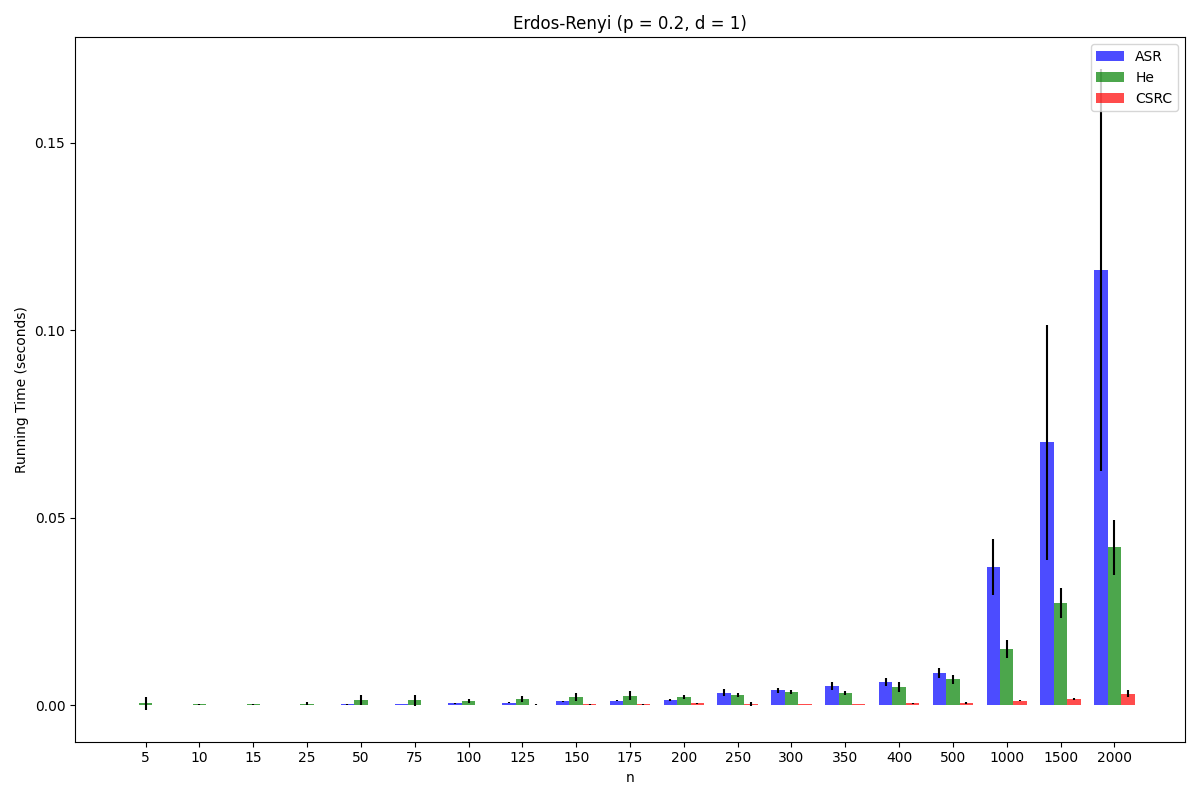
\includegraphics[width=0.49\textwidth]{figures/Figure_1.png}}
	\hfill
	\subfigure[Plot 2]{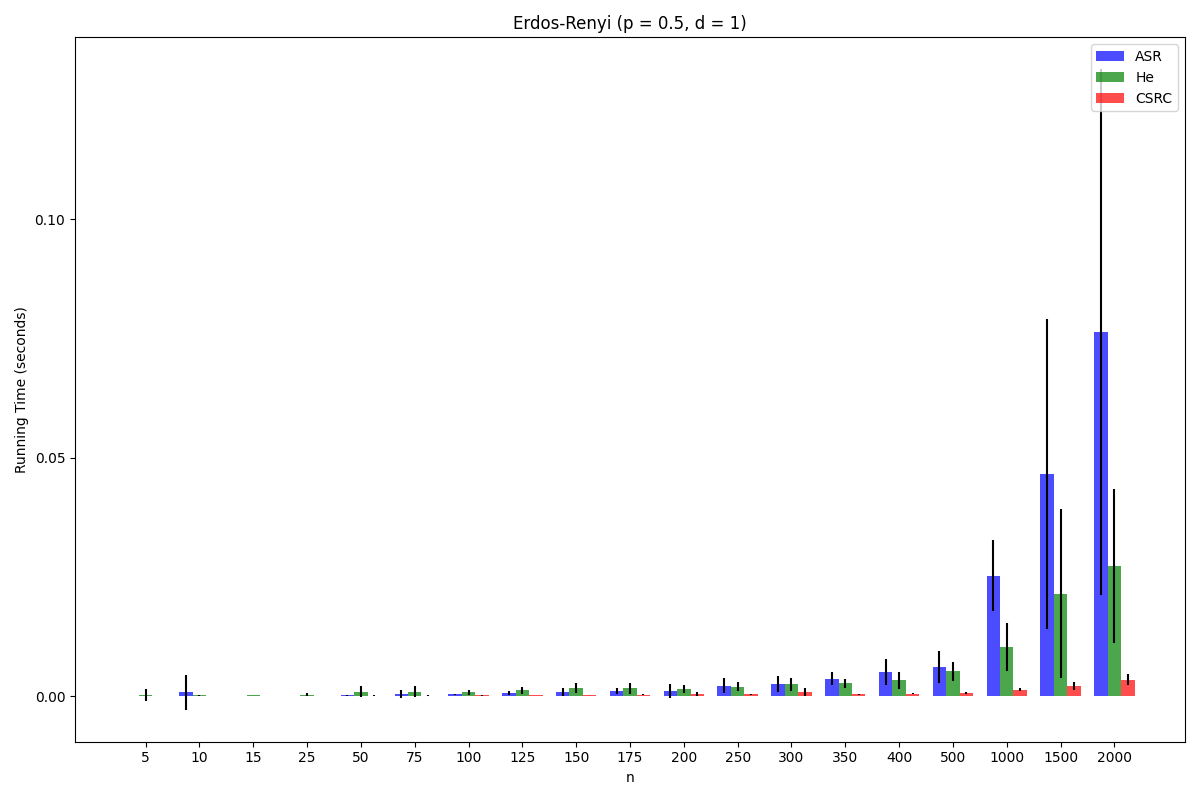
\includegraphics[width=0.49\textwidth]{figures/Figure_2.png}}
	
	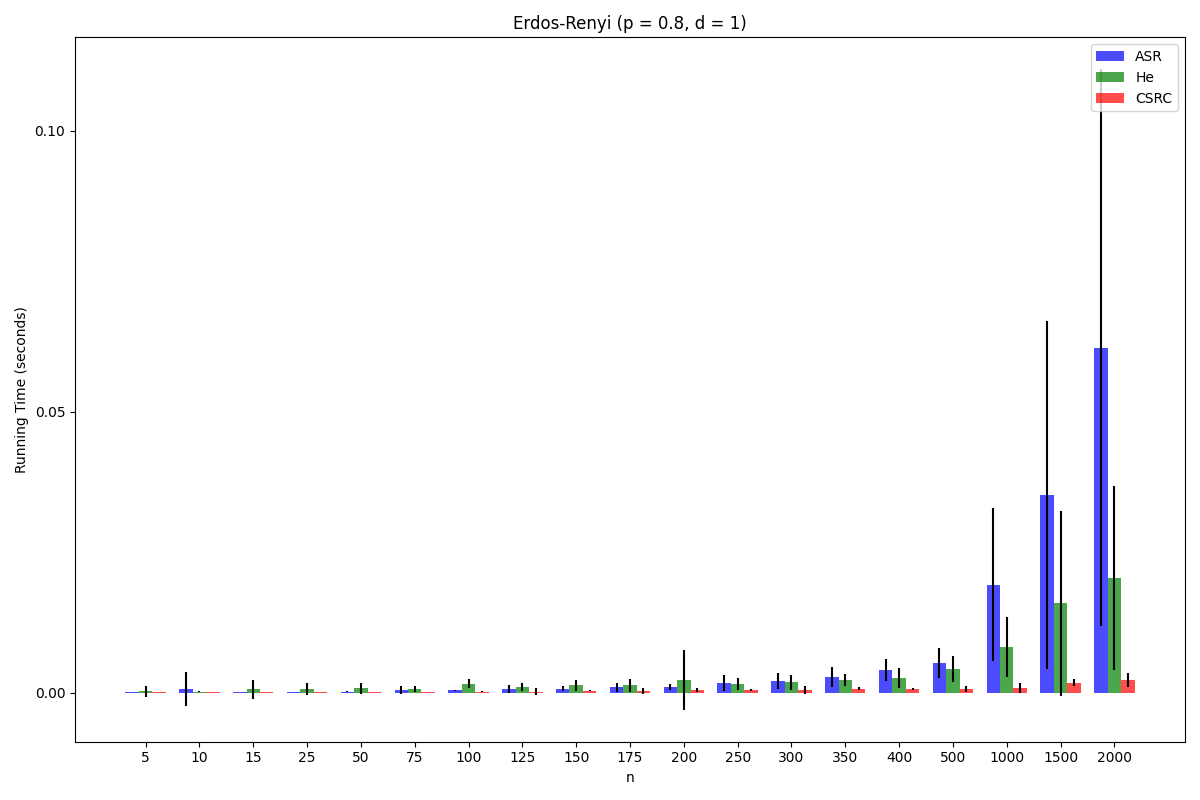
\includegraphics[width=0.49\textwidth]{figures/Figure_3.png}
	
	\caption{Running time plots for each algorithm (Ali-Spirtes-Richardson (ASR) in blue, Hu-Evans (He) in green and Constructive-SRC (CSRC) in red) for Erd\H{o}s-R\'{e}nyi MAGs with $d=1$ and $p=0.2$~(Figure (a)), $p=0.5$~(Figure (b)), $p=0.8$~(Figure (c)).}
	\label{fig:er-1-ap}
\end{figure}

\begin{figure}[htbp]
	\centering
	\subfigure[Plot 1]{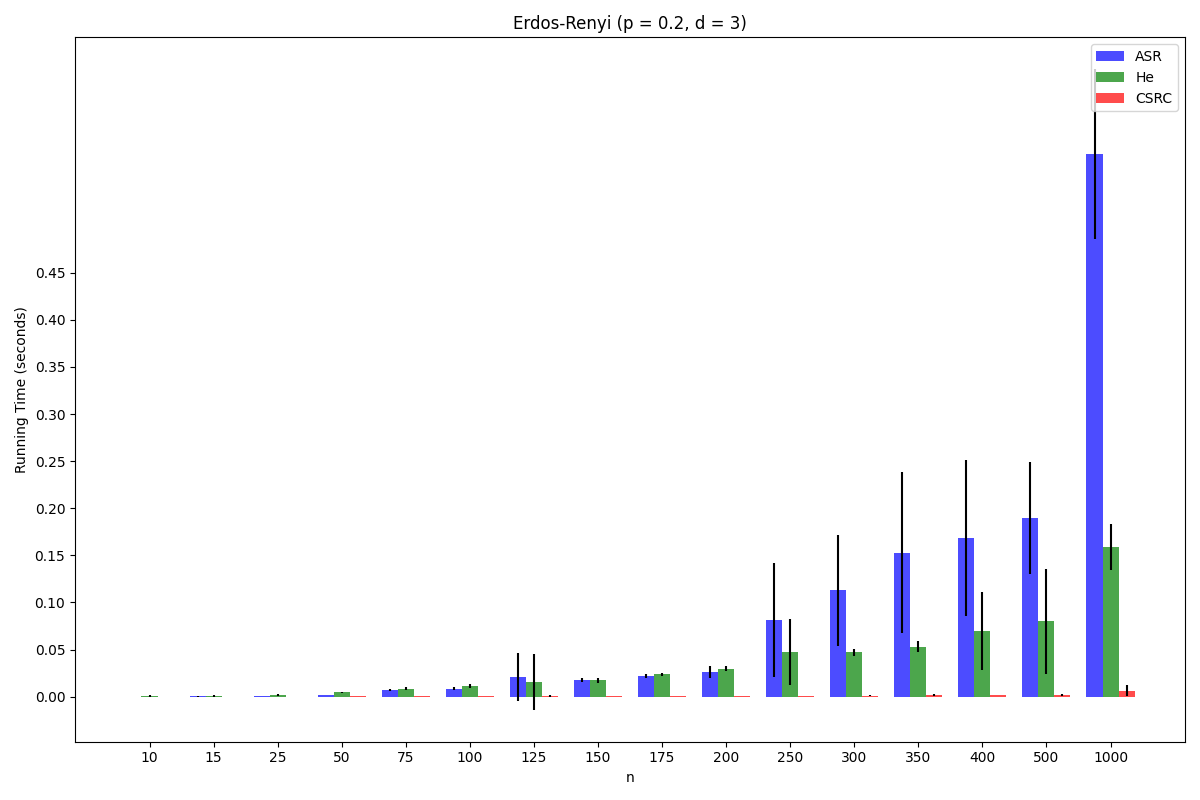
\includegraphics[width=0.49\textwidth]{figures/Figure_4.png}}
	\hfill
	\subfigure[Plot 2]{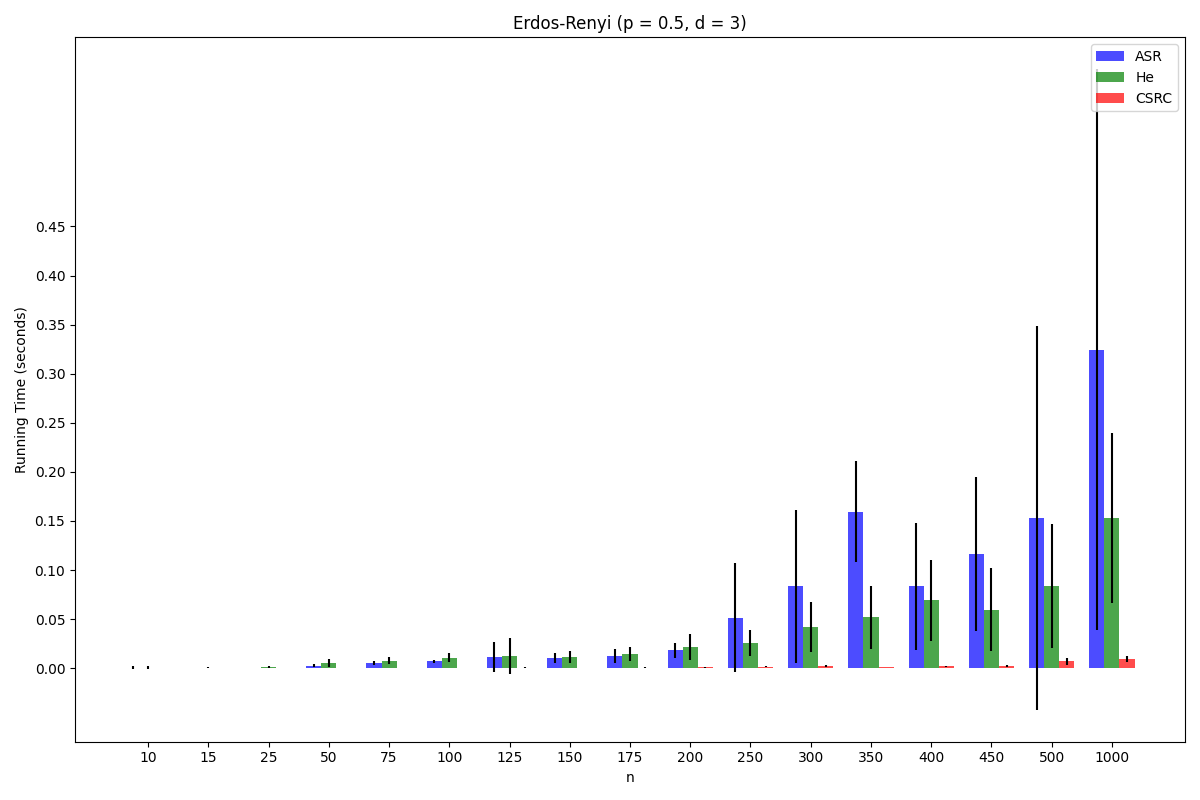
\includegraphics[width=0.49\textwidth]{figures/Figure_5.png}}
	
	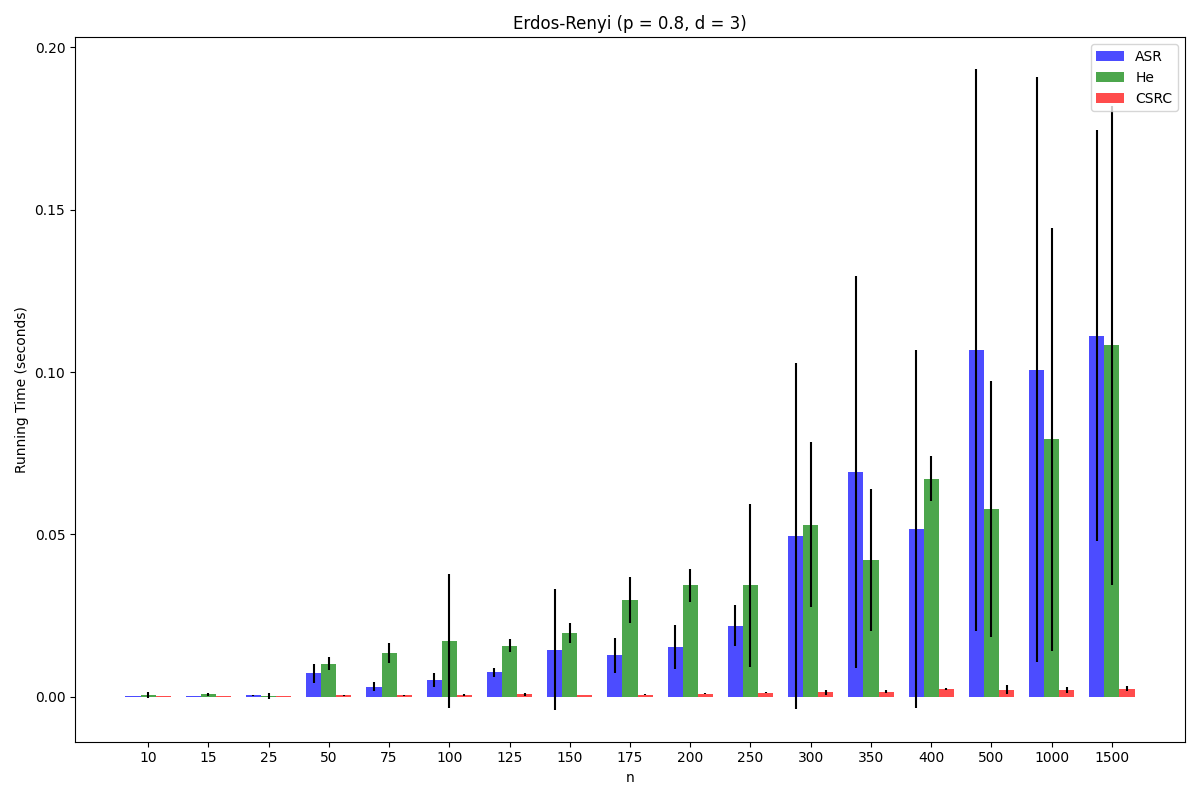
\includegraphics[width=0.49\textwidth]{figures/Figure_6.png}
	
	\caption{Running time plots for each algorithm (Ali-Spirtes-Richardson (ASR) in blue, Hu-Evans (He) in green and Constructive-SRC (CSRC) in red) for Erd\H{o}s-R\'{e}nyi MAGs with $d=3$ and $p=0.2$~(Figure (a)), $p=0.5$~(Figure (b)), $p=0.8$~(Figure (c)).}
	\label{fig:er-3-ap}
\end{figure}

\begin{figure}[htbp]
	\centering
	\subfigure[Plot 1]{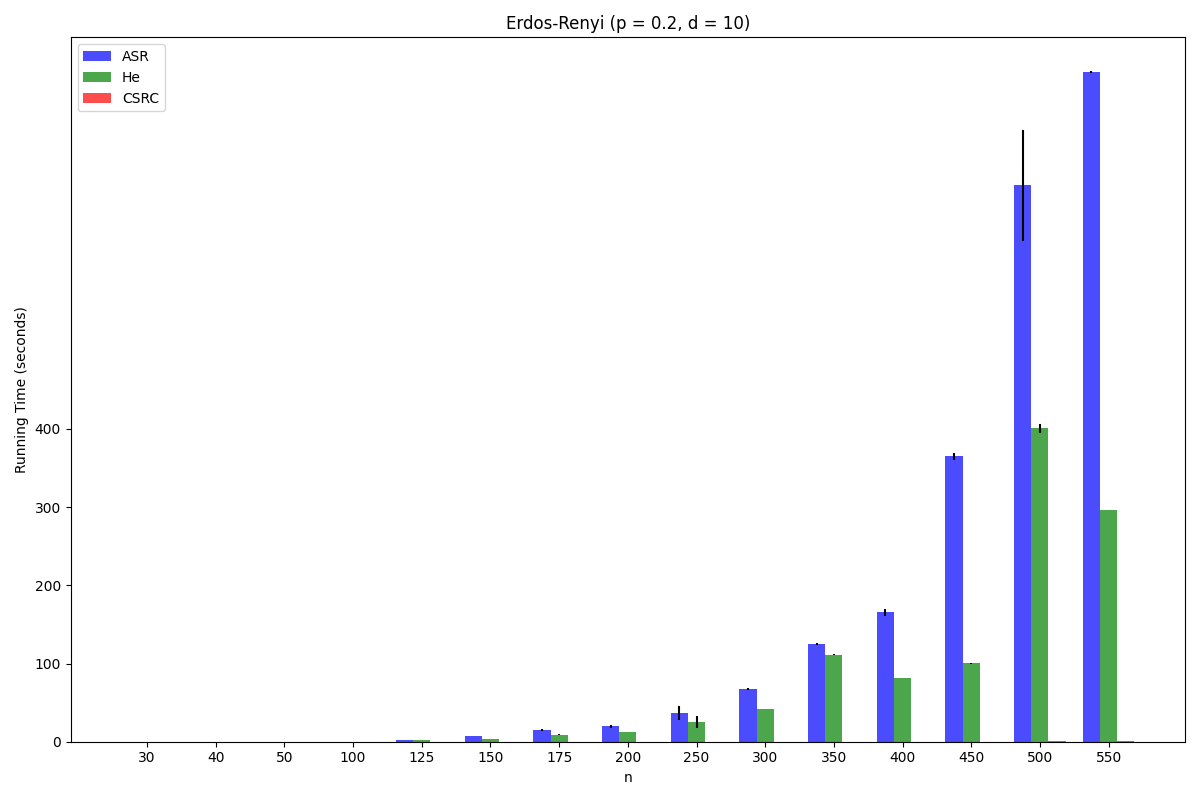
\includegraphics[width=0.49\textwidth]{figures/Figure_7.png}}
	\hfill
	\subfigure[Plot 2]{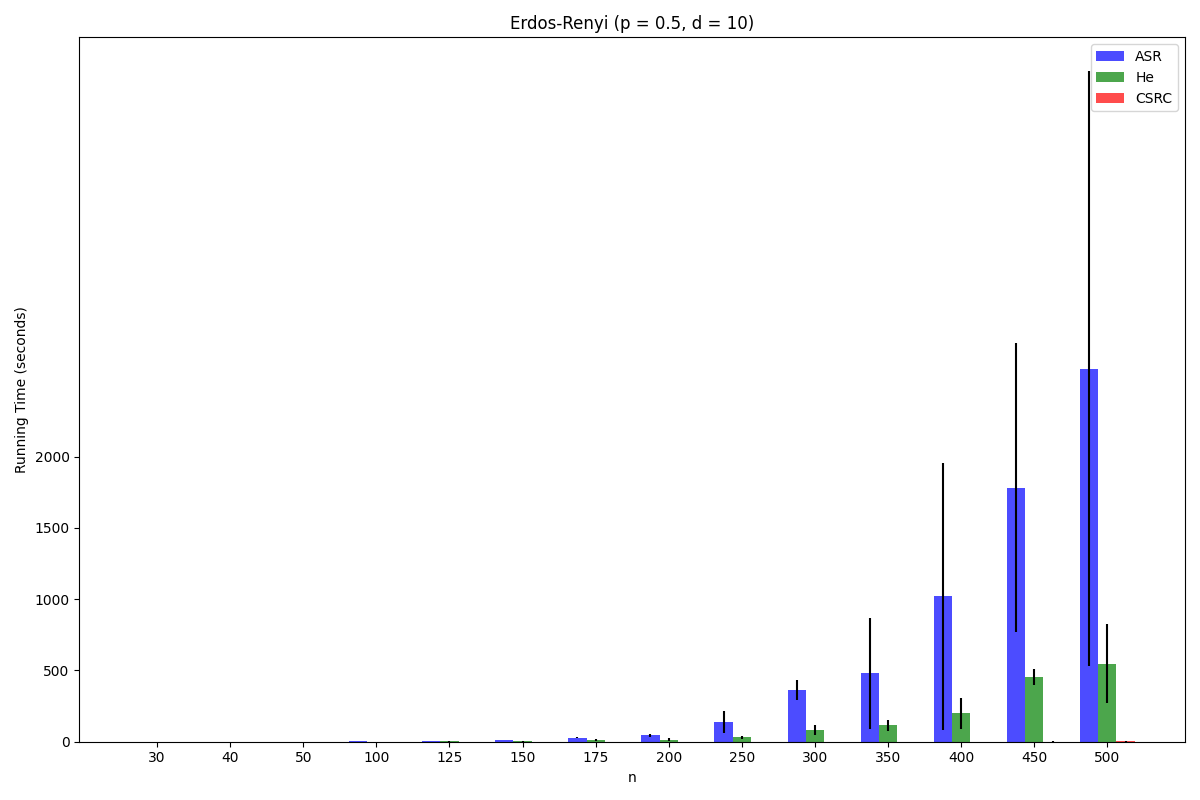
\includegraphics[width=0.49\textwidth]{figures/Figure_8.png}}
	
	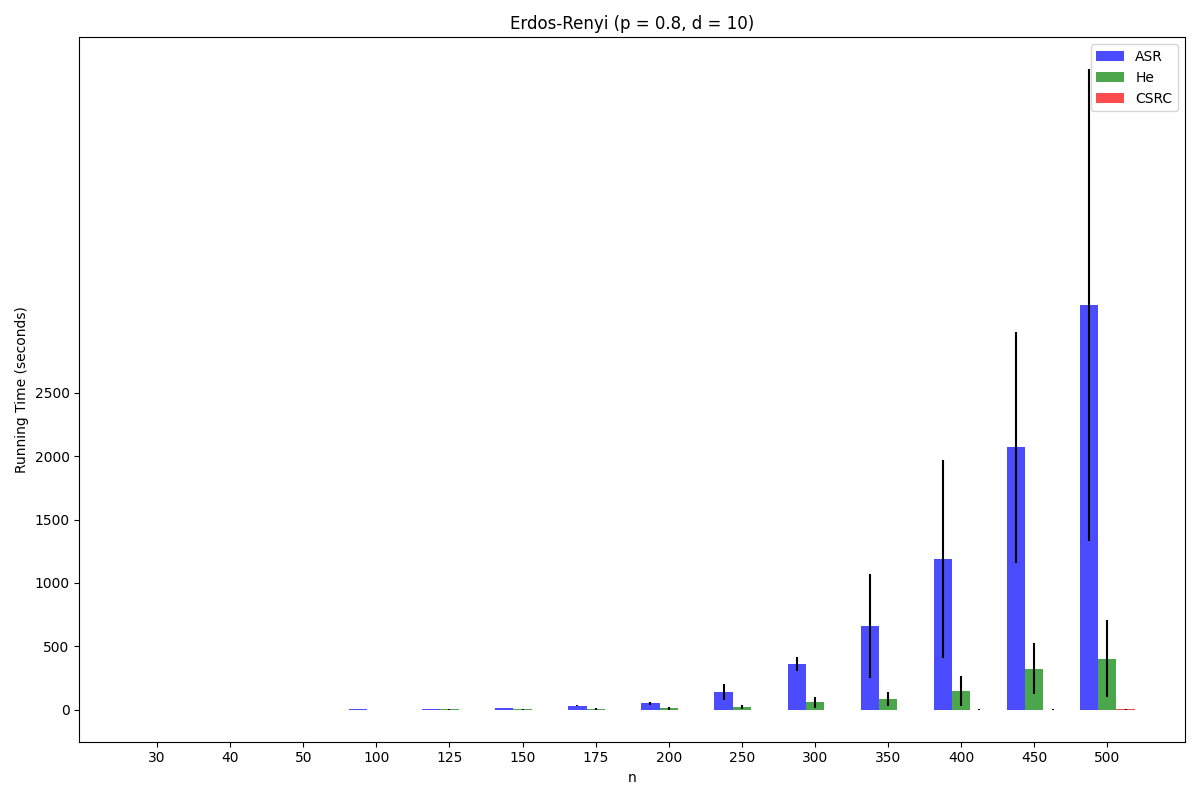
\includegraphics[width=0.49\textwidth]{figures/Figure_9.png}
	
	\caption{Running time plots for each algorithm (Ali-Spirtes-Richardson (ASR) in blue, Hu-Evans (He) in green and Constructive-SRC (CSRC) in red) for Erd\H{o}s-R\'{e}nyi MAGs with $d=10$ and $p=0.2$~(Figure (a)), $p=0.5$~(Figure (b)), $p=0.8$~(Figure (c)).}
	\label{fig:er-10-ap}
\end{figure}

\begin{figure}[htbp]
	\centering
	\subfigure[Plot 1]{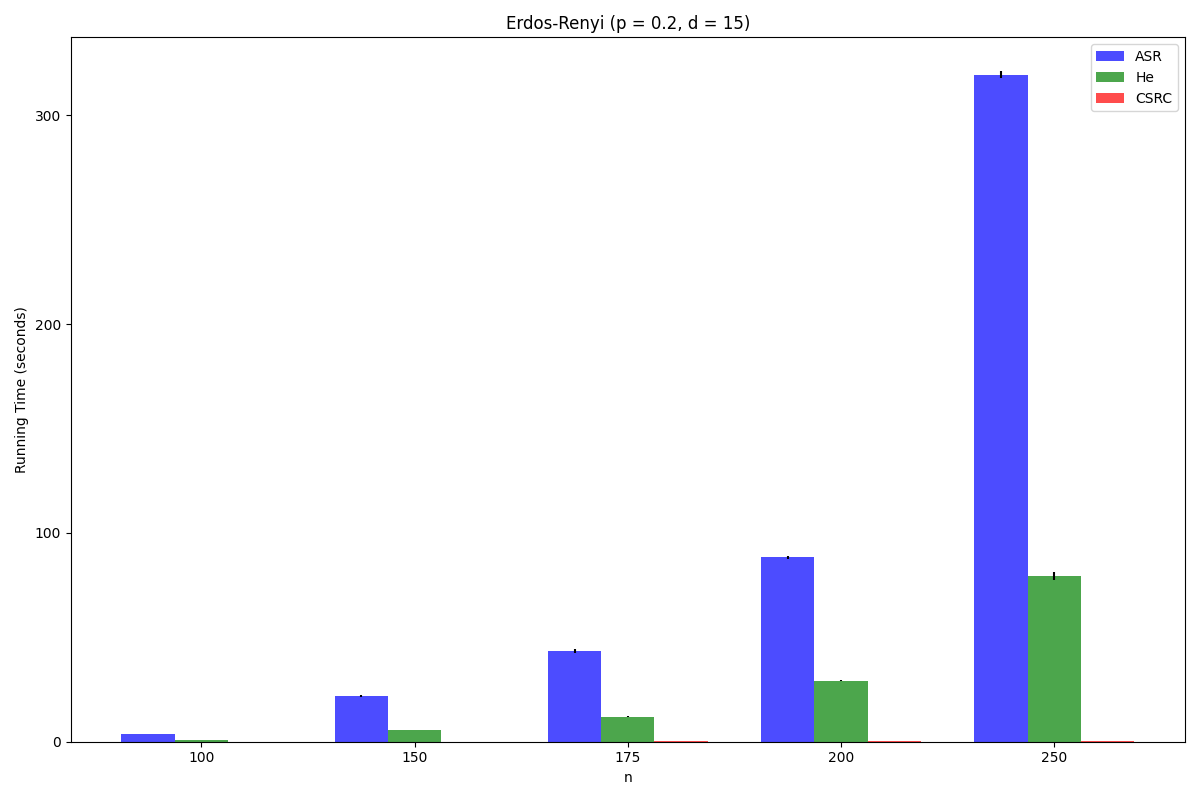
\includegraphics[width=0.49\textwidth]{figures/Figure_10.png}}
	\hfill
	\subfigure[Plot 2]{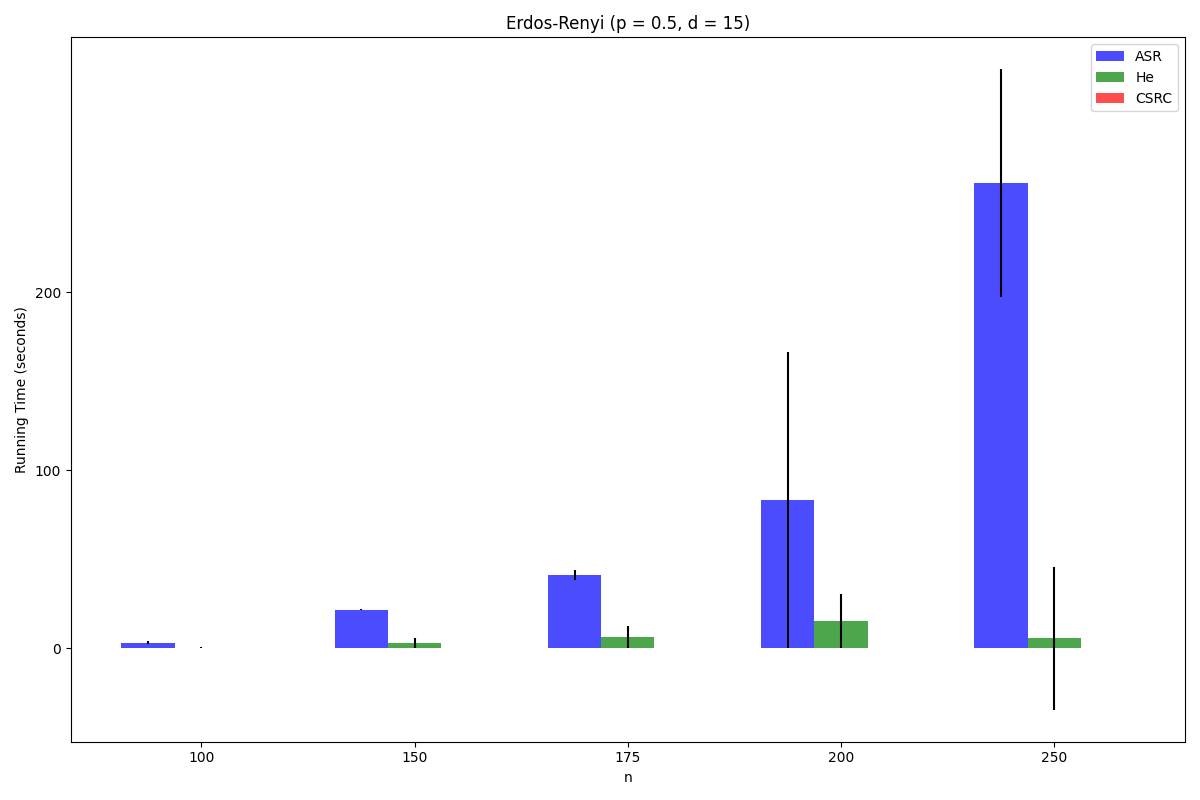
\includegraphics[width=0.49\textwidth]{figures/Figure_11.png}}
	
	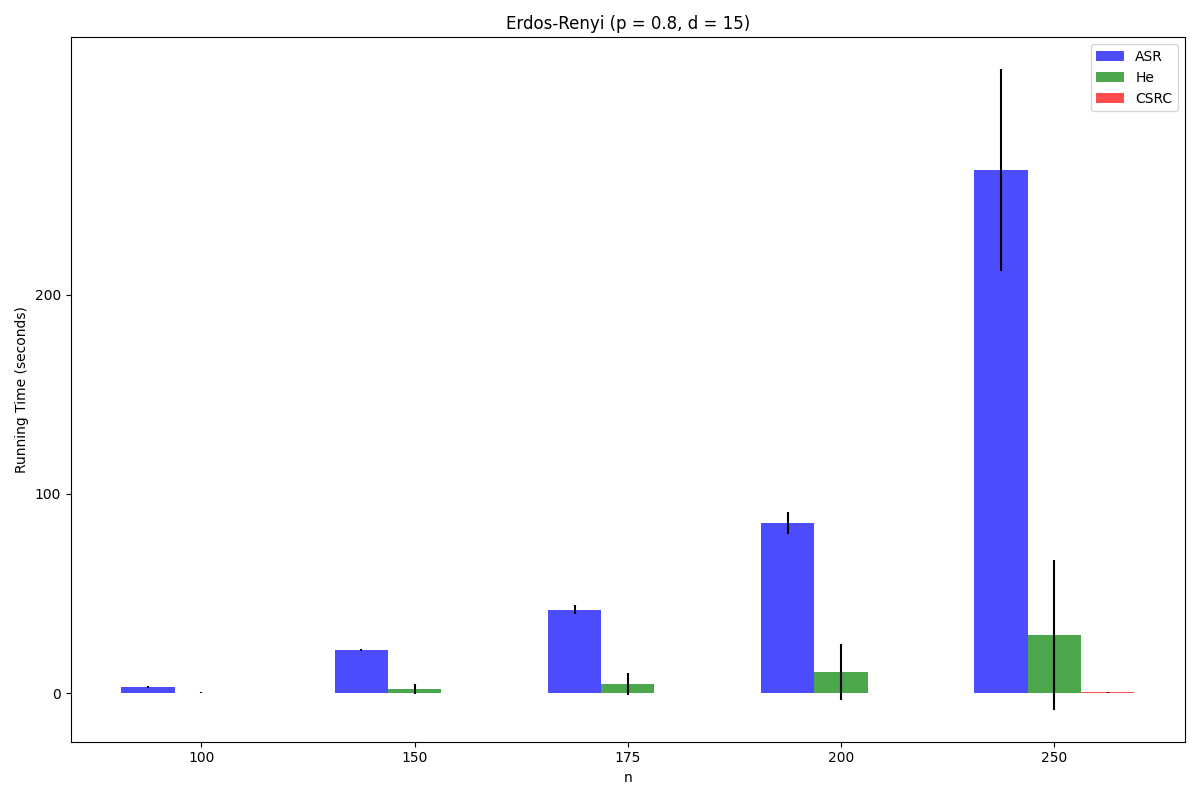
\includegraphics[width=0.49\textwidth]{figures/Figure_12.png}
	
	\caption{Running time plots for each algorithm (Ali-Spirtes-Richardson (ASR) in blue, Hu-Evans (He) in green and Constructive-SRC (CSRC) in red) for Erd\H{o}s-R\'{e}nyi MAGs with $d=15$ and $p=0.2$~(Figure (a)), $p=0.5$~(Figure (b)), $p=0.8$~(Figure (c)).}
	\label{fig:er-15-ap}
\end{figure}

\begin{figure}[htbp]
	\centering
	\subfigure[Plot 1]{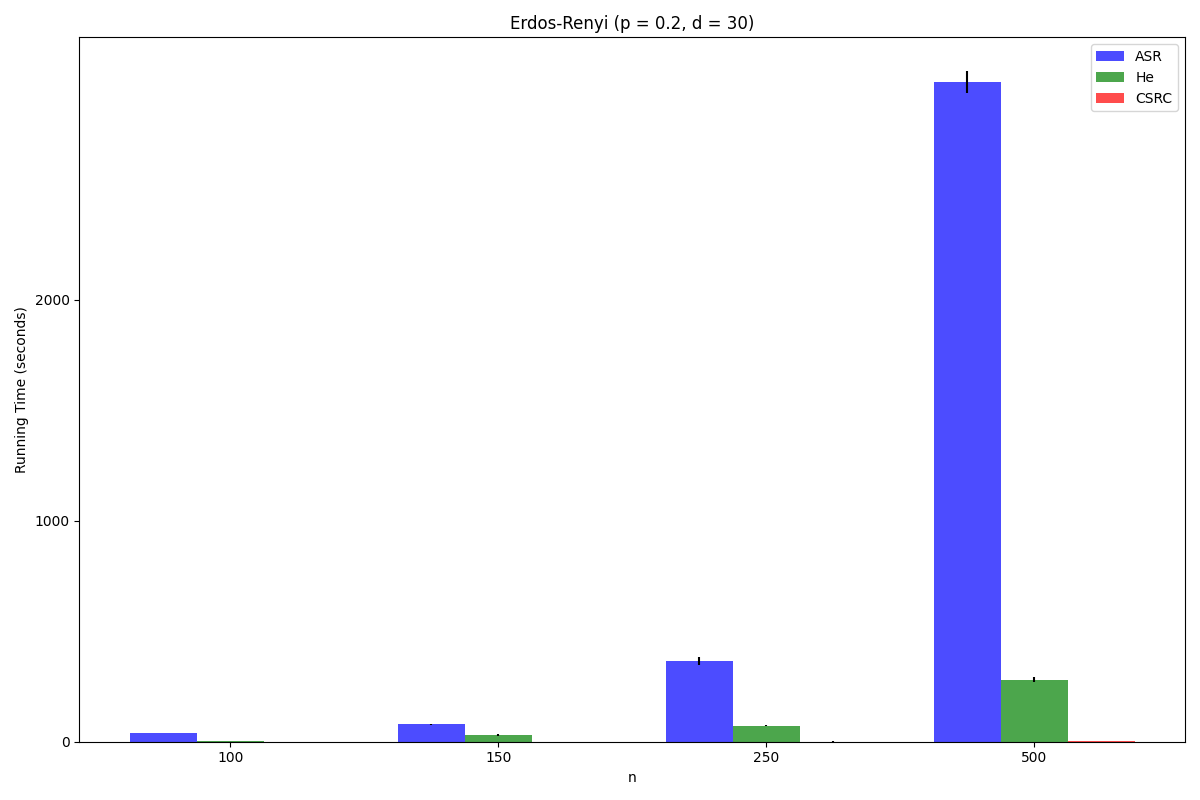
\includegraphics[width=0.49\textwidth]{figures/Figure_13.png}}
	\hfill
	\subfigure[Plot 2]{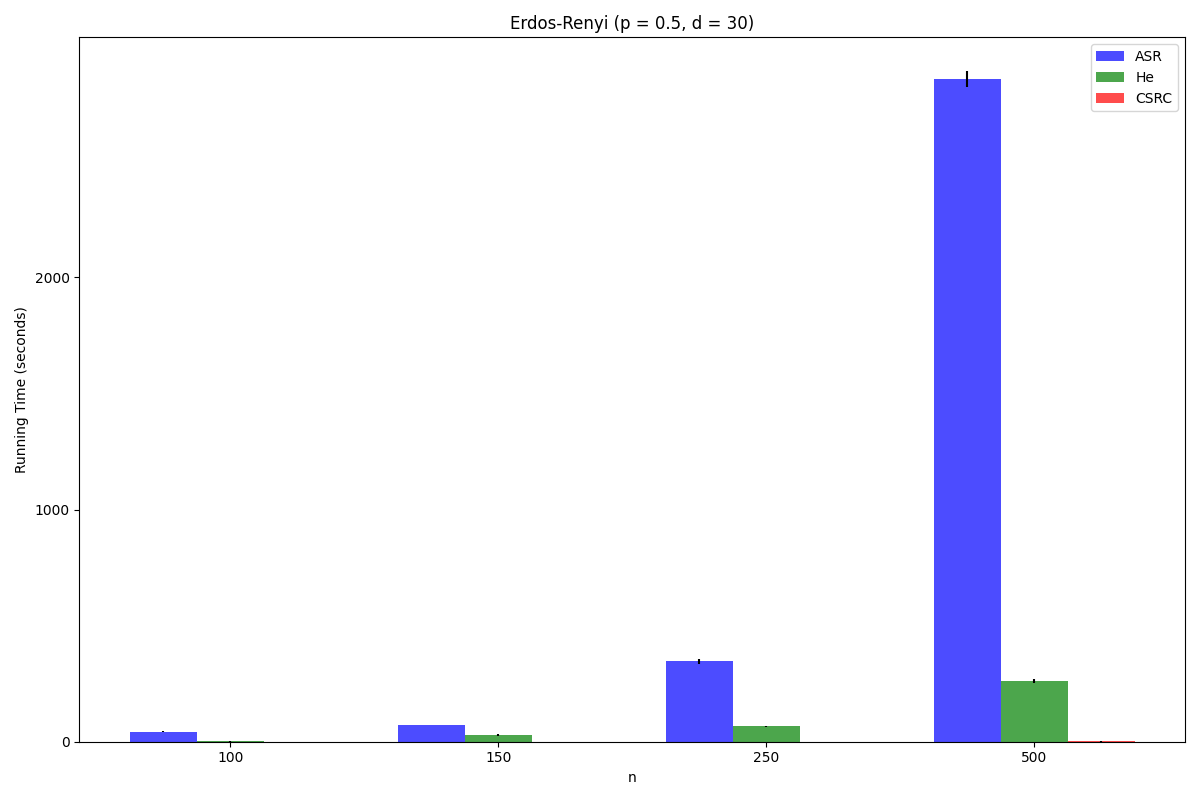
\includegraphics[width=0.49\textwidth]{figures/Figure_14.png}}
	
	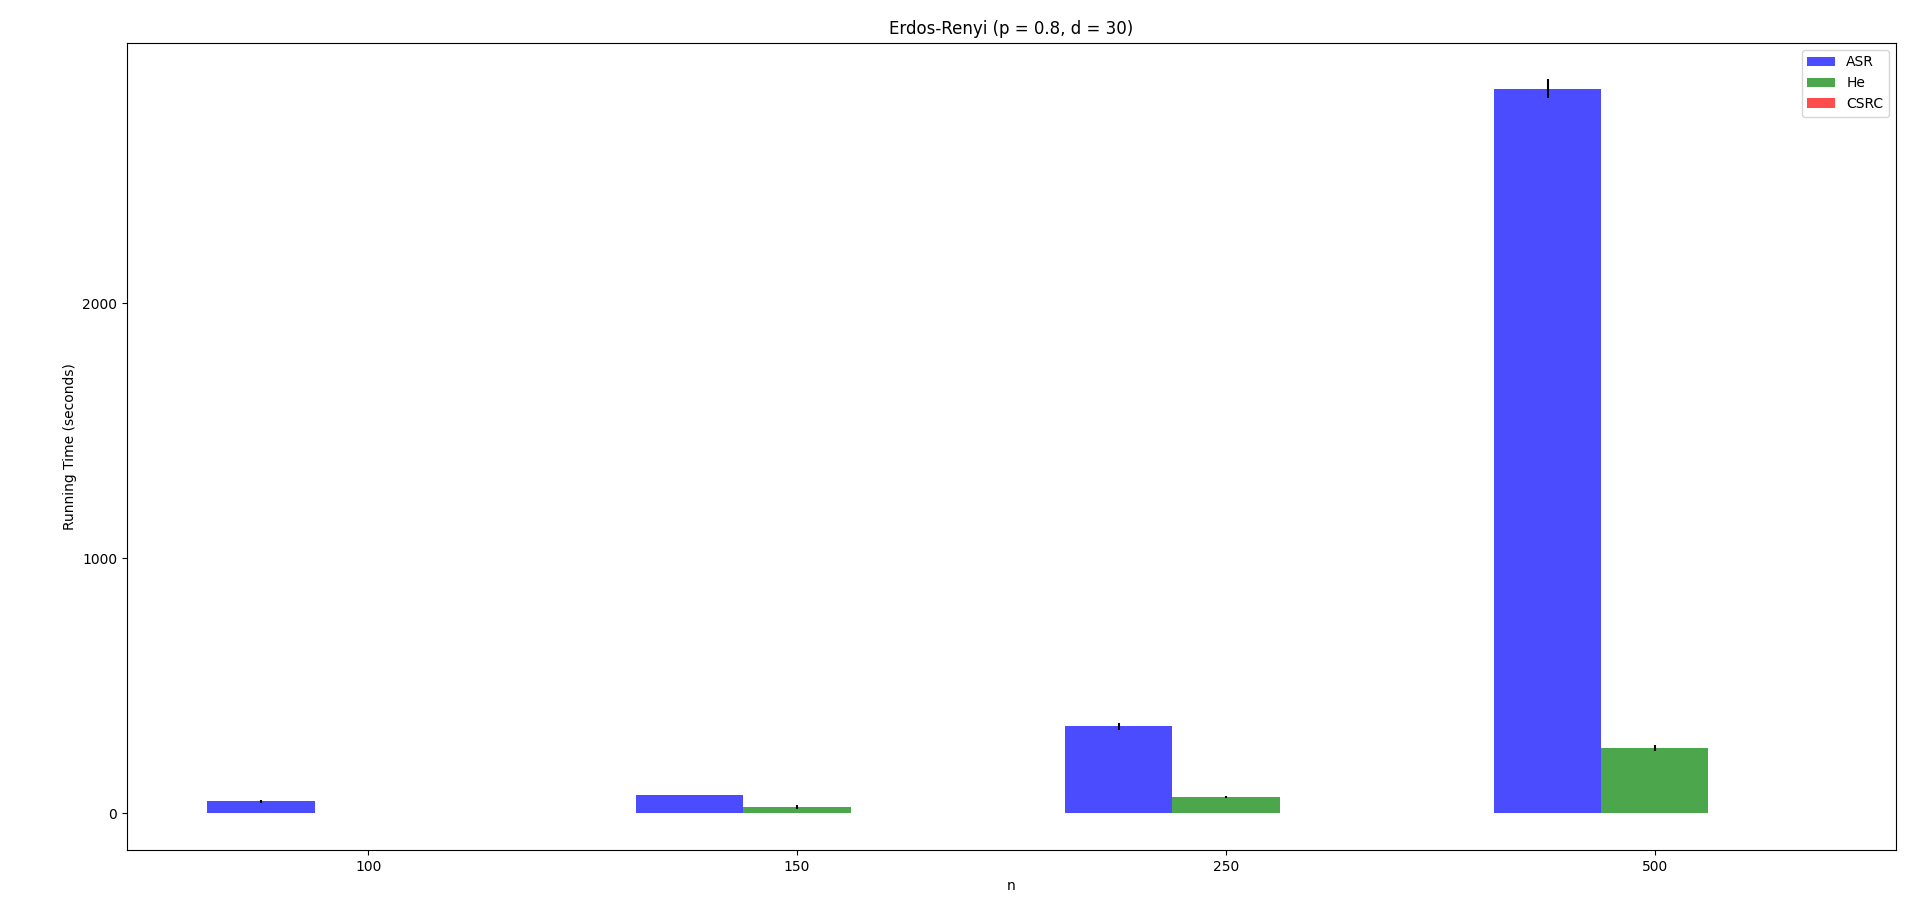
\includegraphics[width=0.49\textwidth]{figures/Figure_15.png}
	
	\caption{Running time plots for each algorithm (Ali-Spirtes-Richardson (ASR) in blue, Hu-Evans (He) in green and Constructive-SRC (CSRC) in red) for Erd\H{o}s-R\'{e}nyi MAGs with $d=30$ and $p=0.2$~(Figure (a)), $p=0.5$~(Figure (b)), $p=0.8$~(Figure (c)).}
	\label{fig:er-30-ap}
\end{figure}

\pagebreak
\subsection{Plots for the Barab\'{a}si-Albert model}

\begin{figure}[htbp]
	\centering
	\subfigure[Plot 1]{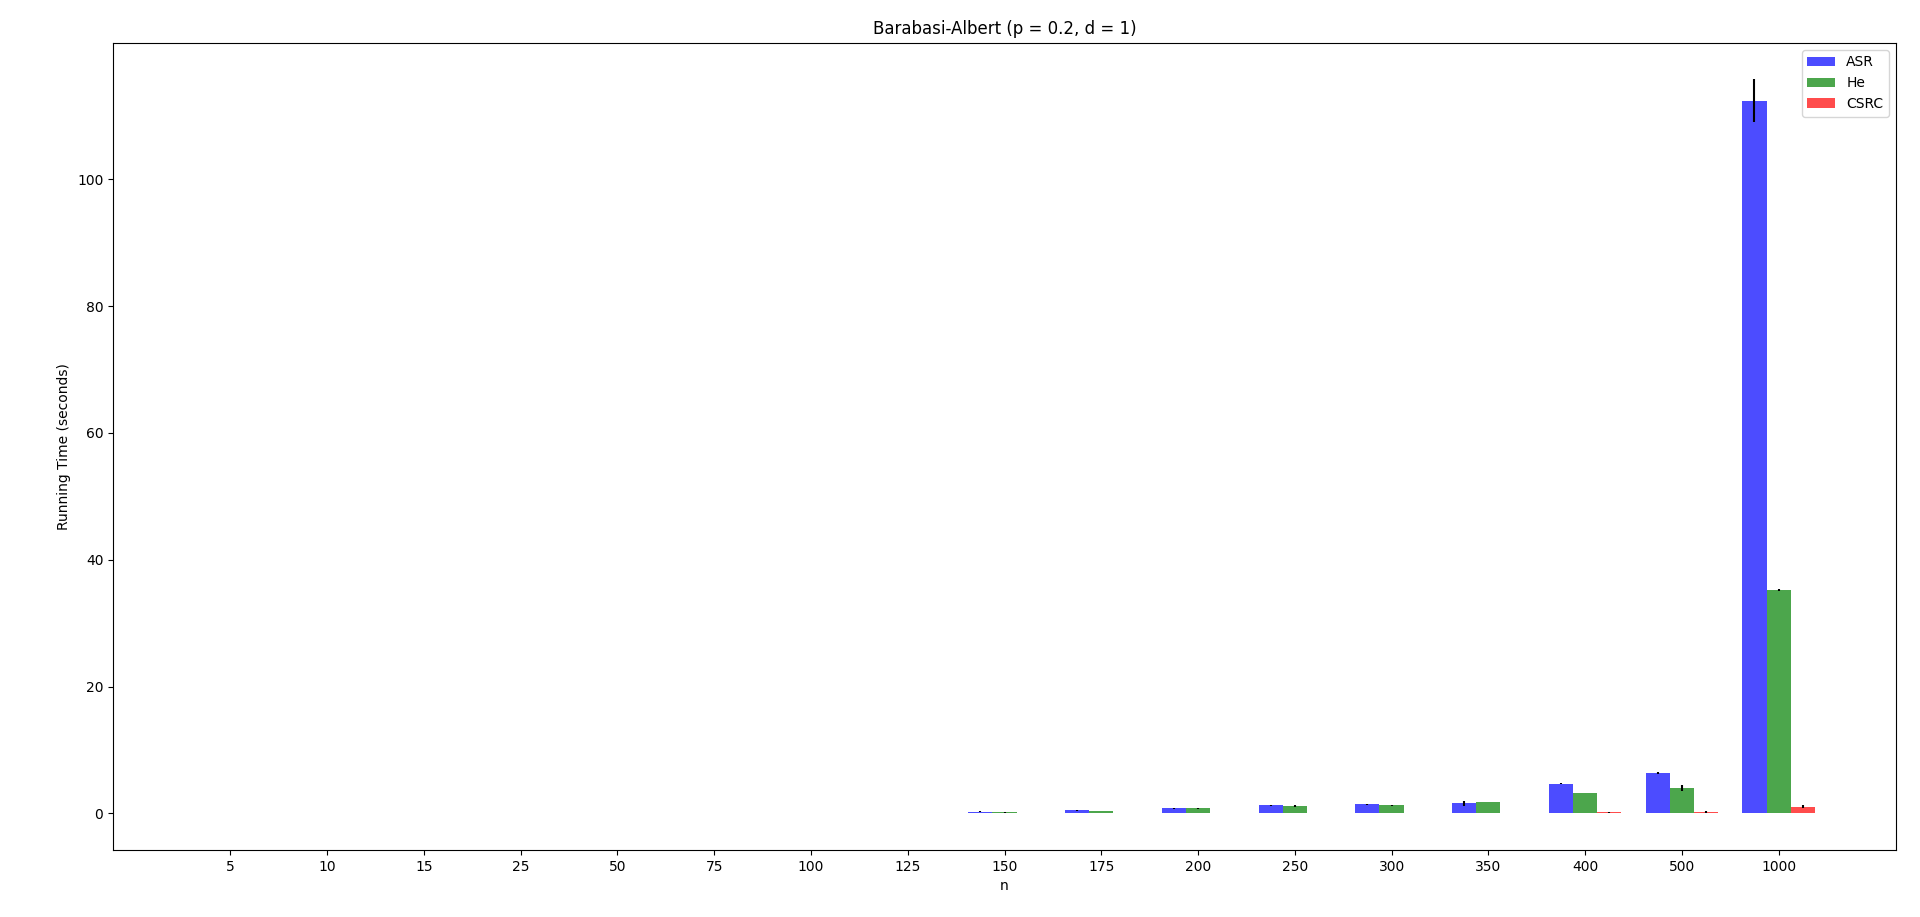
\includegraphics[width=0.49\textwidth]{figures/Figure_16.png}}
	\hfill
	\subfigure[Plot 2]{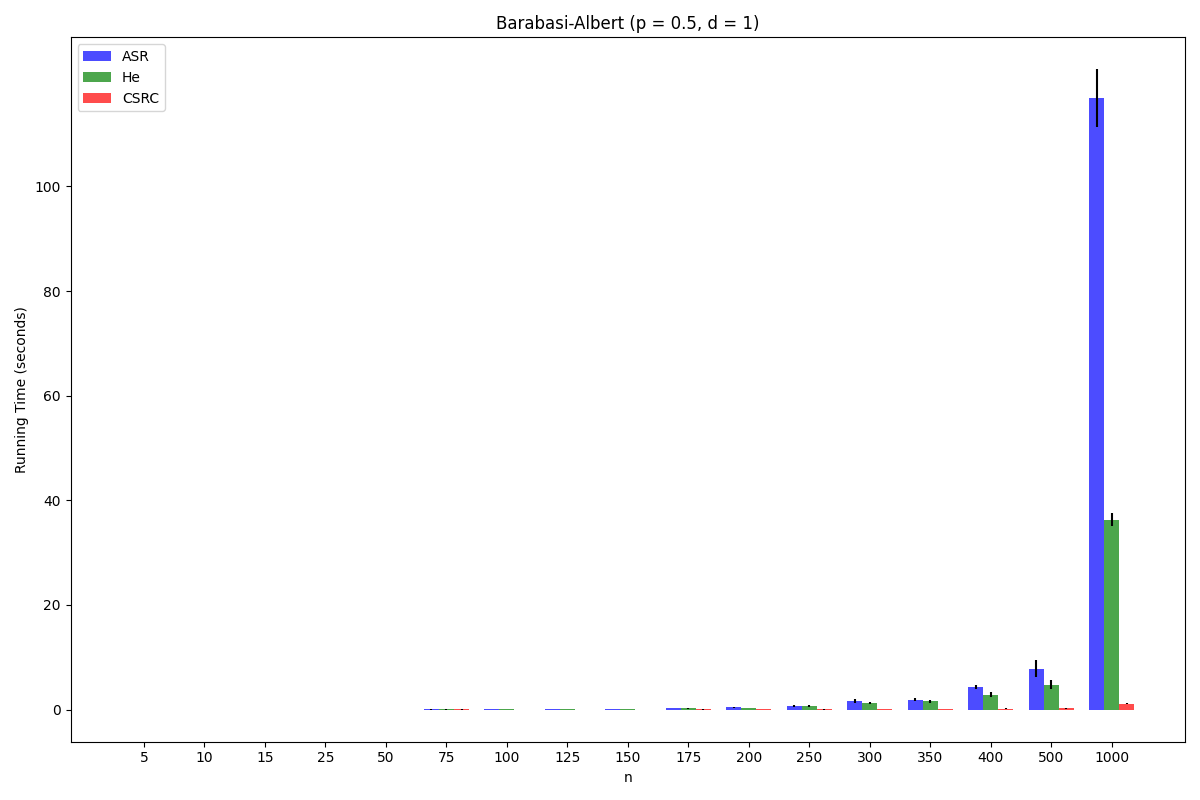
\includegraphics[width=0.49\textwidth]{figures/Figure_17.png}}
	
	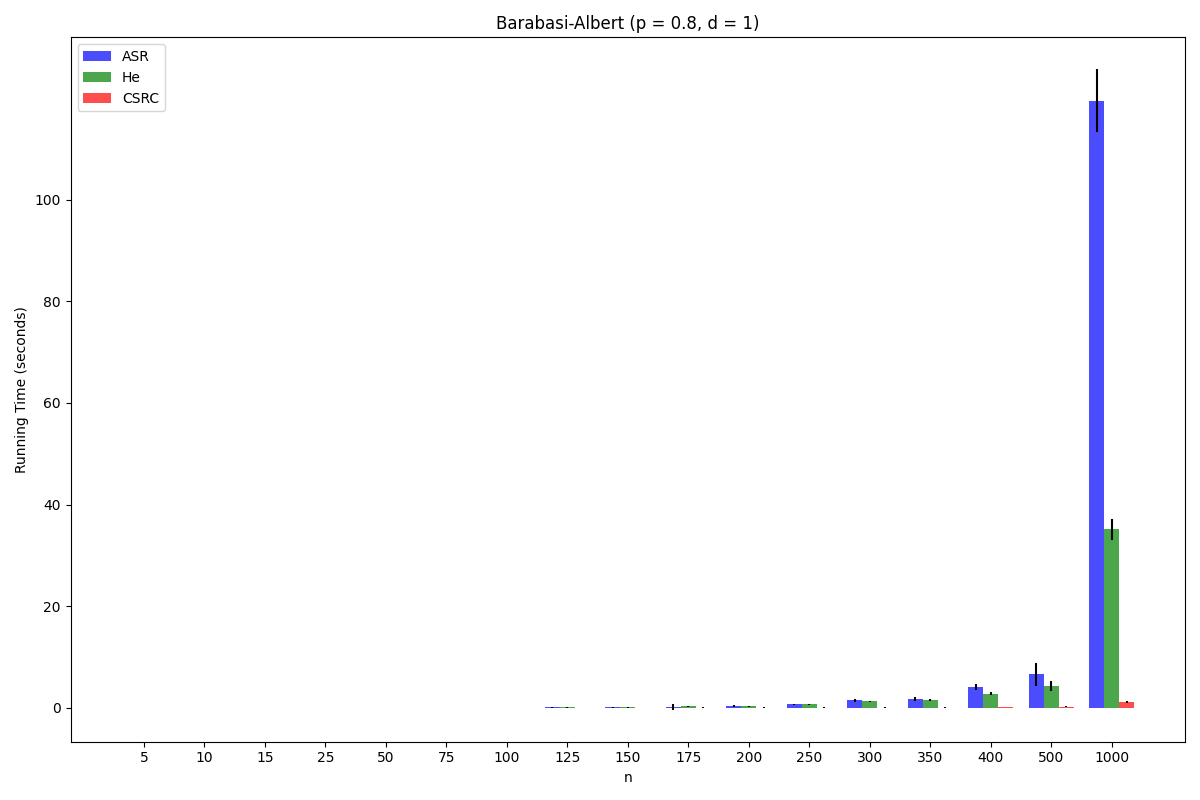
\includegraphics[width=0.49\textwidth]{figures/Figure_18.png}
	
	\caption{Running time plots for each algorithm (Ali-Spirtes-Richardson (ASR) in blue, Hu-Evans (He) in green and Constructive-SRC (CSRC) in red) for Barabasi-Albert MAGs with $d=1$ and $p=0.2$~(Figure (a)), $p=0.5$~(Figure (b)), $p=0.8$~(Figure (c)).}
	\label{fig:sf-1-ap}
\end{figure}

\begin{figure}[htbp]
	\centering
	\subfigure[Plot 1]{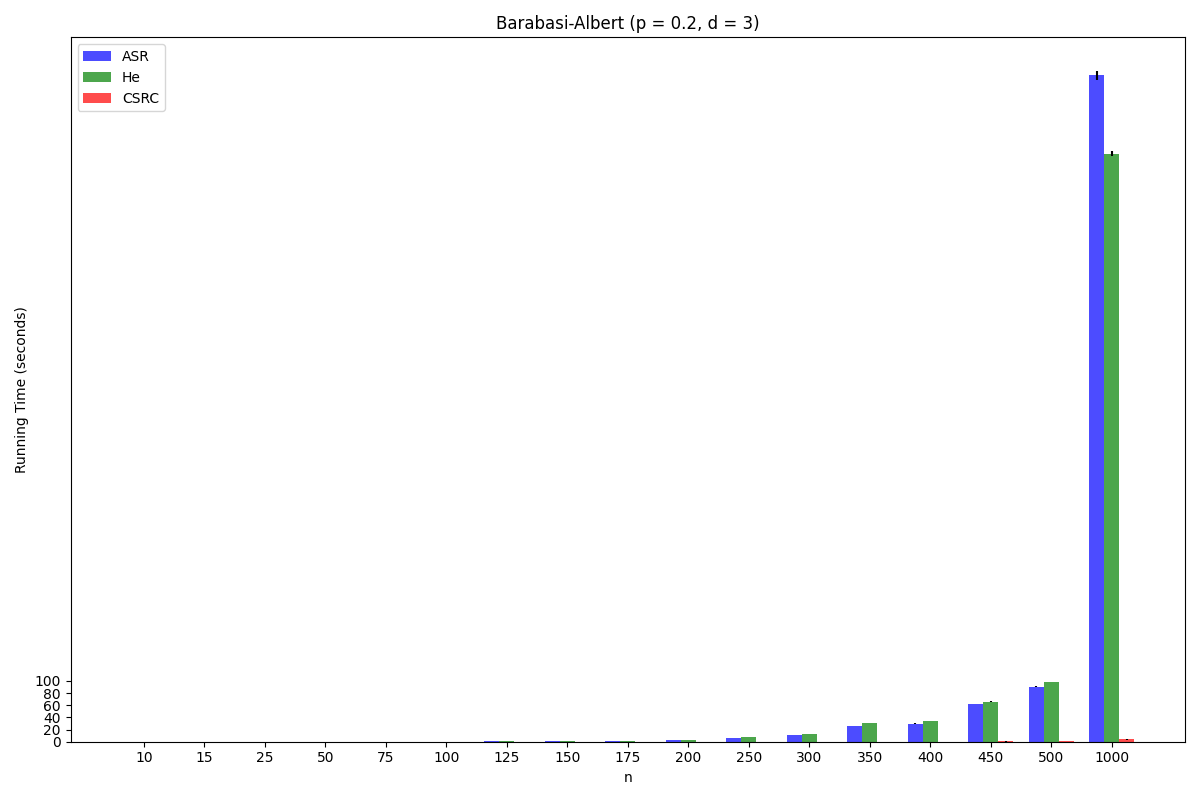
\includegraphics[width=0.49\textwidth]{figures/Figure_19.png}}
	\hfill
	\subfigure[Plot 2]{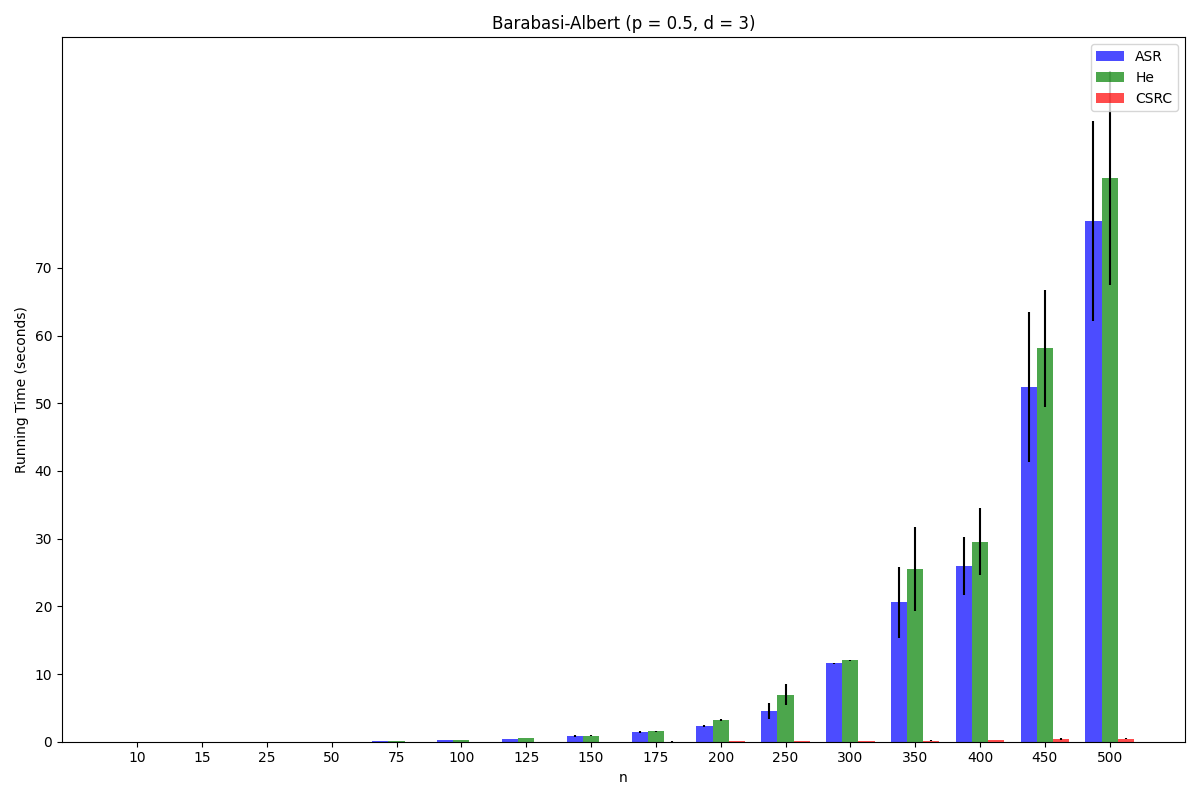
\includegraphics[width=0.49\textwidth]{figures/Figure_20.png}}
	
	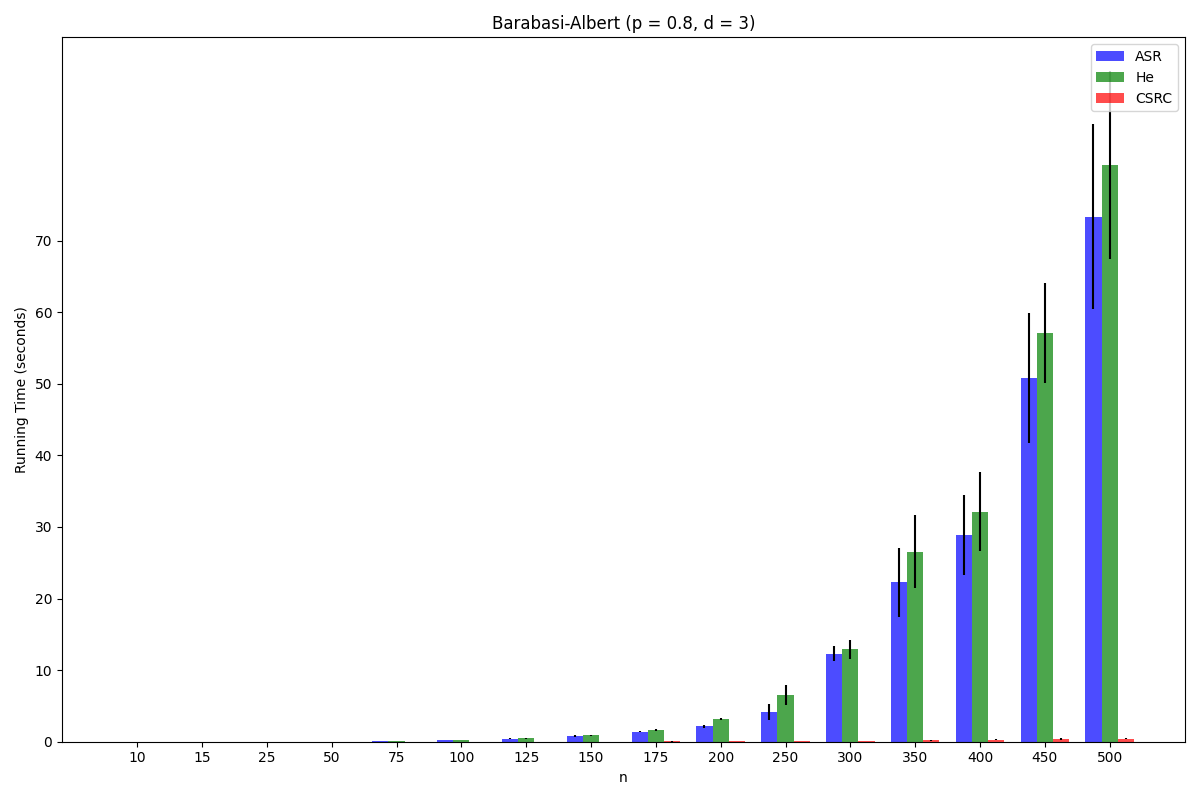
\includegraphics[width=0.49\textwidth]{figures/Figure_21.png}
	
	\caption{Running time plots for each algorithm (Ali-Spirtes-Richardson (ASR) in blue, Hu-Evans (He) in green and Constructive-SRC (CSRC) in red) for Barabasi-Albert MAGs with $d=3$ and $p=0.2$~(Figure (a)), $p=0.5$~(Figure (b)), $p=0.8$~(Figure (c)).}
	\label{fig:sf-3-ap}
\end{figure}

\begin{figure}[htbp]
	\centering
	\subfigure[Plot 1]{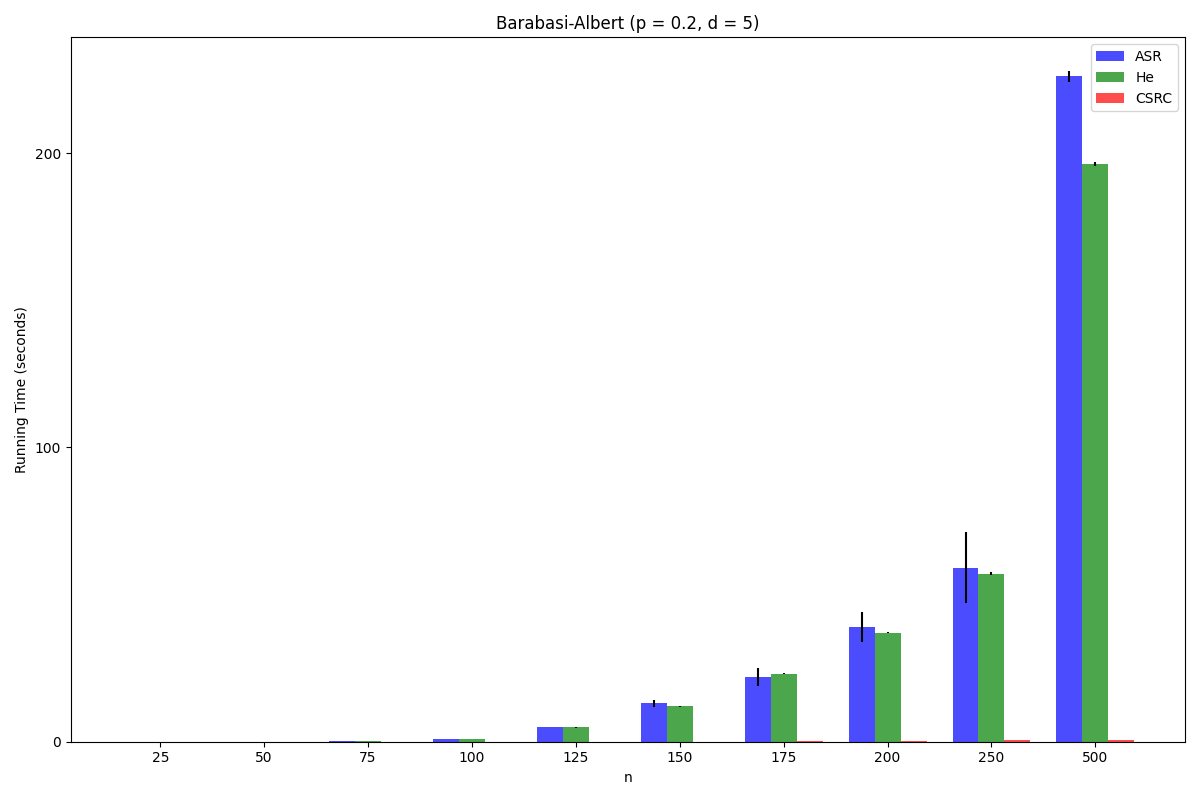
\includegraphics[width=0.49\textwidth]{figures/Figure_22.png}}
	\hfill
	\subfigure[Plot 2]{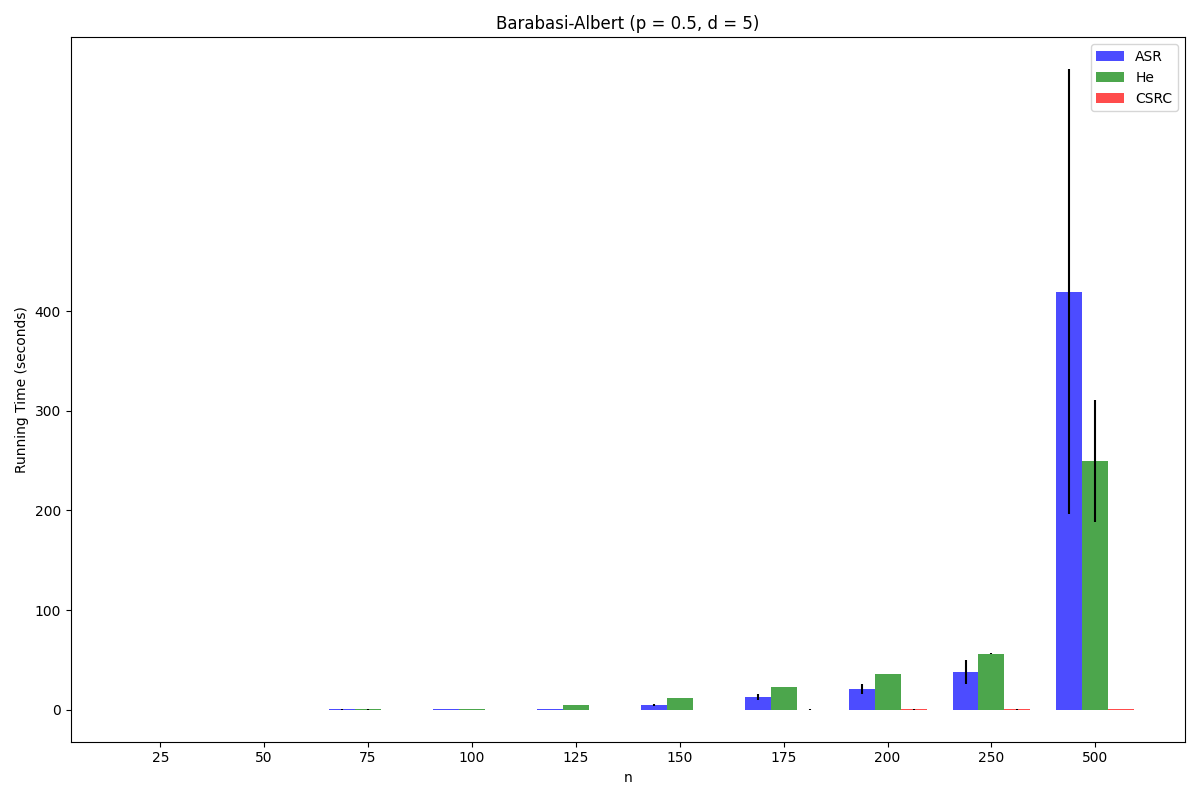
\includegraphics[width=0.49\textwidth]{figures/Figure_23.png}}
	
	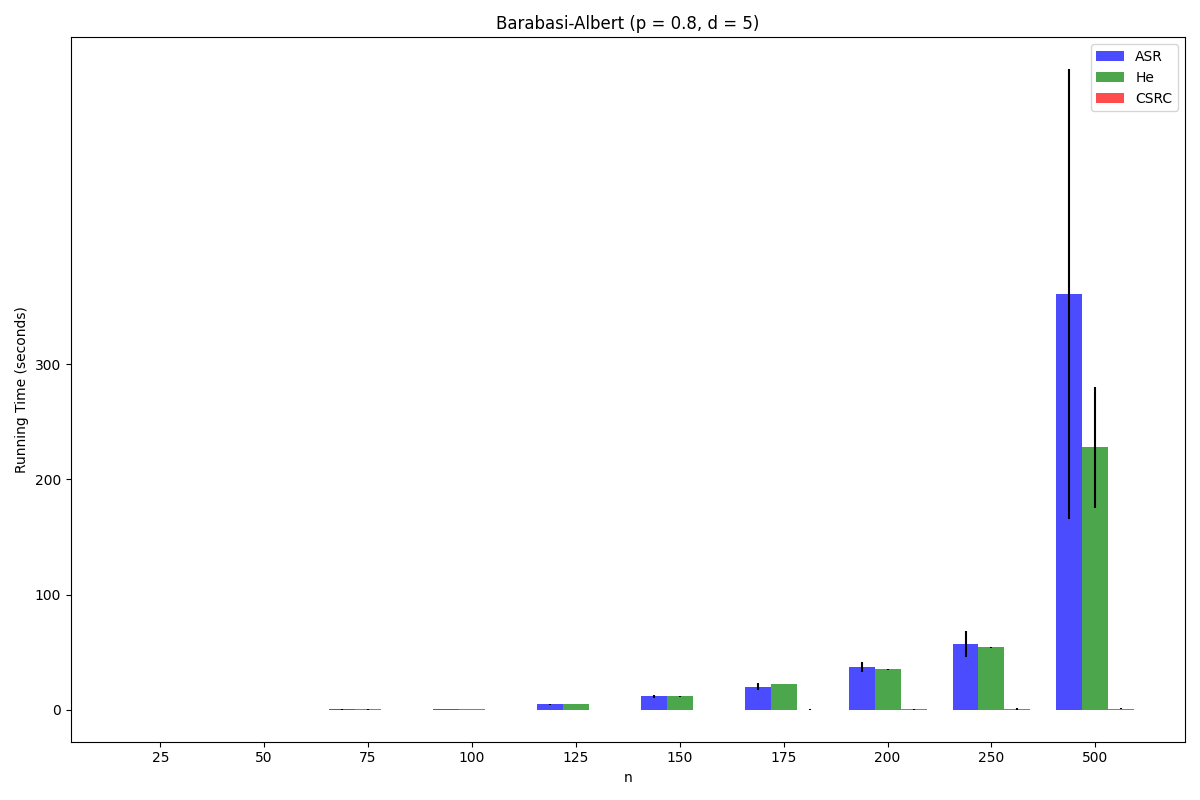
\includegraphics[width=0.49\textwidth]{figures/Figure_24.png}
	
	\caption{Running time plots for each algorithm (Ali-Spirtes-Richardson (ASR) in blue, Hu-Evans (He) in green and Constructive-SRC (CSRC) in red) for Barabasi-Albert MAGs with $d=5$ and $p=0.2$~(Figure (a)), $p=0.5$~(Figure (b)), $p=0.8$~(Figure (c)).}
	\label{fig:sf-5-ap}
\end{figure}

\begin{figure}[htbp]
	\centering
	\subfigure[Plot 1]{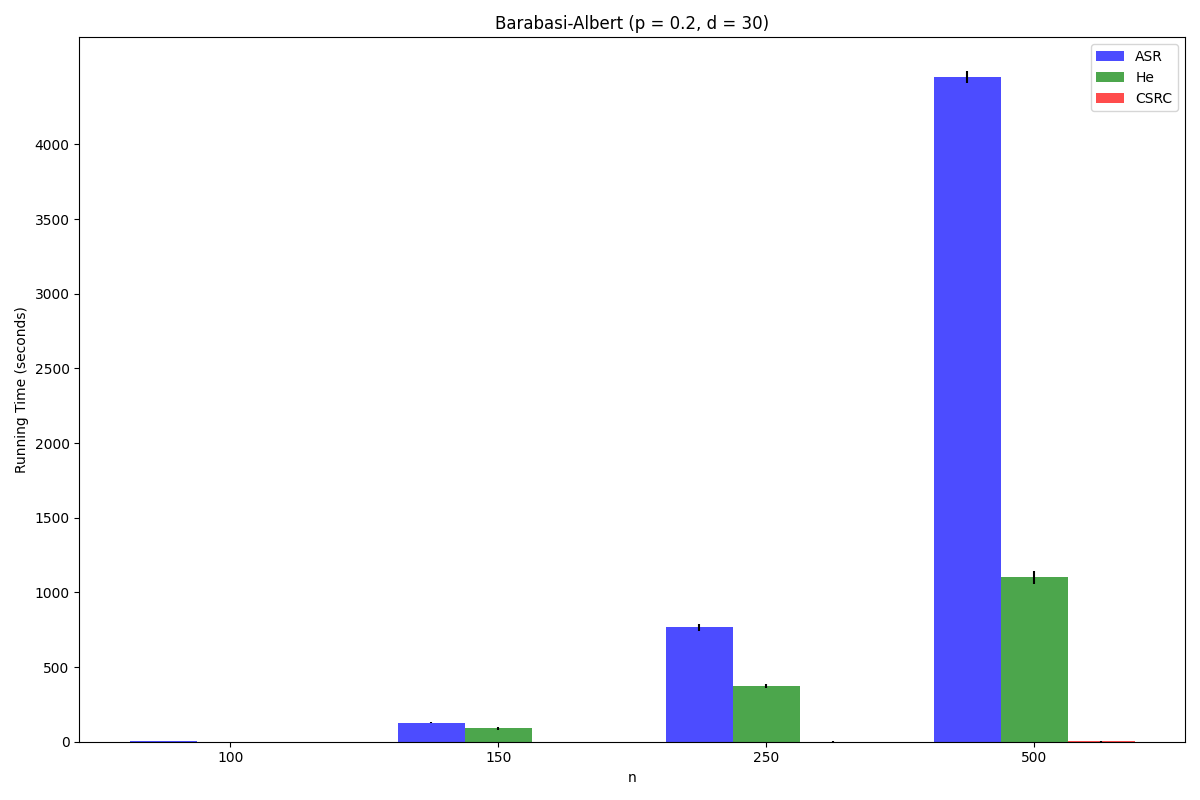
\includegraphics[width=0.49\textwidth]{figures/Figure_25.png}}
	\hfill
	\subfigure[Plot 2]{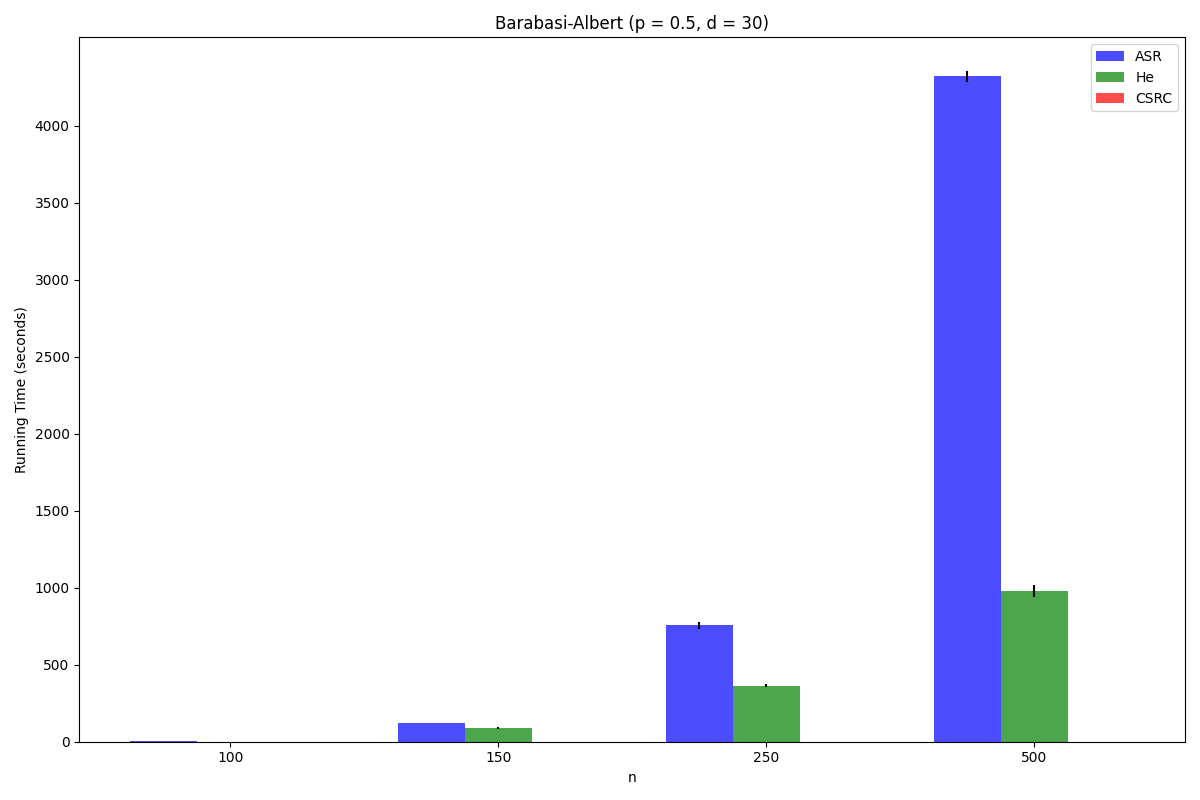
\includegraphics[width=0.49\textwidth]{figures/Figure_26.png}}
	
	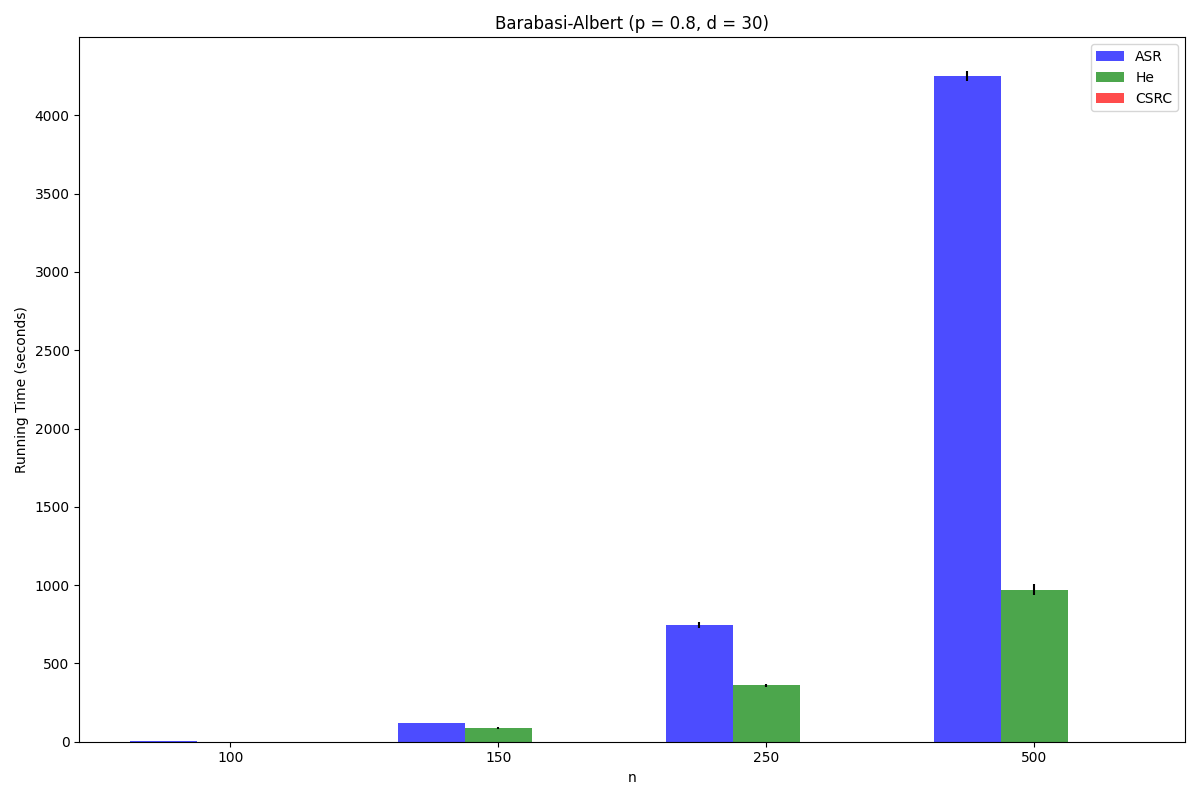
\includegraphics[width=0.49\textwidth]{figures/Figure_27.png}
	
	\caption{Running time plots for each algorithm (Ali-Spirtes-Richardson (ASR) in blue, Hu-Evans (He) in green and Constructive-SRC (CSRC) in red) for Barabasi-Albert MAGs with $d=30$ and $p=0.2$~(Figure (a)), $p=0.5$~(Figure (b)), $p=0.8$~(Figure (c)).}
	\label{fig:sf-30-ap}
\end{figure}

\end{document}
